The careful analysis of the experimental data will allow for the calculation of the number of events observed in a specific region of phase space, which combined with the luminosity determined from beam charge accumulated on the Faraday cup, provides a rudimentary estimate of the differential \xsec. However, many corrections need to be applied to this raw calculation to arrive at a more accurate result. The most dominant correction term is known as ``acceptance'' which can be thought of as the ratio of the number of events that are experimentally detected relative to the number that truly occurred. In this work we will use ``acceptance'' to refer to a combination of geometrical acceptance (the fraction of 4$\pi$ surface area covered by the detector systems), detector efficiency, and track reconstruction efficiency. This correction term (and others) are best estimated by creating a simulation of the physics experiment with computational means, and using the ratio of the number of detected simulated events to the number of generated simulated events as an approximation to the true acceptance, \eqref{eq:acceptance}. 



  \begin{equation}\labelAndRemember{eq:acceptance}
                   {\epsilon_{acc} = \frac{N_{detected,experiment}}{N_{truth}} \approx  \frac{N_{detected,simulation}}{N_{truth,simulation}}  \equiv \frac{N_{sim}}{N_{gen}} = \hat{\epsilon}_{acc}}.
             \end{equation}      
             

Here $\hat{\epsilon}_{acc}$ is the estimator for the true acceptance, $\epsilon_{acc}$. For the remainder of this work, we will refer to the number of events detected in the real-world experiment as \Nexp, those produced in the real-world as \Ntruth, those detected in the simulation as \Nsim, and those generated for simulation as \Ngen.  

Several components are necessary to arrive at a computational estimate of $\epsilon_{acc}$ and other correction factors. They are: 

\begin{itemize}
    \item A model of the true underlying physics processes to produce \Ngen \secref{sec:ch3generator}
    \item A method to simulate the experiment to produce \Nsim \secref{sec:sim_pipeline}
    \item Sufficient computational infrastructure to perform the calculations \secref{sec:comp_infrastructure}
\end{itemize}



\iffalse
Approaching through the lens of an inverse problem, we use existing knowledge to create event generators that produce reasonable the underlying physics processes. These computer generated datasets are then swam through microphysics simulations of the CLAS12 experiment on an event by event basis to produce a simulated dataset. By comparing the experimental data to the simulated data, and the simulated data to the model of the underlying distribution, inferences can be made about the true underlying distribution generating the experimental data. 
\todo{Fix this stupidly phrased section}
\fi


\section{Event Generation}\label{sec:ch3generator}
    The event generators used in this work are based on the MAID unitary isobar model \parencite{Tiator2006MAIDTechniques}, \parencite{Dreschsel1992ThresholdNucleons} which concerns the photo and electroproduction of pions off of nucleons. It originated as an ``\textbf{A}mplitudes \textbf{A}nd \textbf{O}bservables '' (AAO) generator that worked in the resonance regime \parencite{Burkert1991AmplitudesGenerator} and was extended to function at higher W based on theoretical models \parencite{Goloskokov2010AnElectroproduction} and validated on experimental data \parencite{Bedlinskiy2014ExclusiveCLAS} as well as used in recent physics results \parencite{Diehl2022MultidimensionalRegion}. 

There are two generators, ``aao\_norad'', which is a nonradiative generator that creates events with an outgoing electron, proton, and two photons from the decay of the neutral pion, and ``aao\_rad'', which incorporates radiative corrections into the event generation and produces events with an outgoing electron, proton, neutral pion, and radiated photon. These two generators were refactored to function under a larger software package \href{https://github.com/JeffersonLab/aao_gen}{aao\_gen} which provides access to both generators in one system. Sample distributions of the nonradiative generator are shown in \ref{fig:aao_norad_gen}.

    \begin{figure}[H]
        \centering
        \subfloat{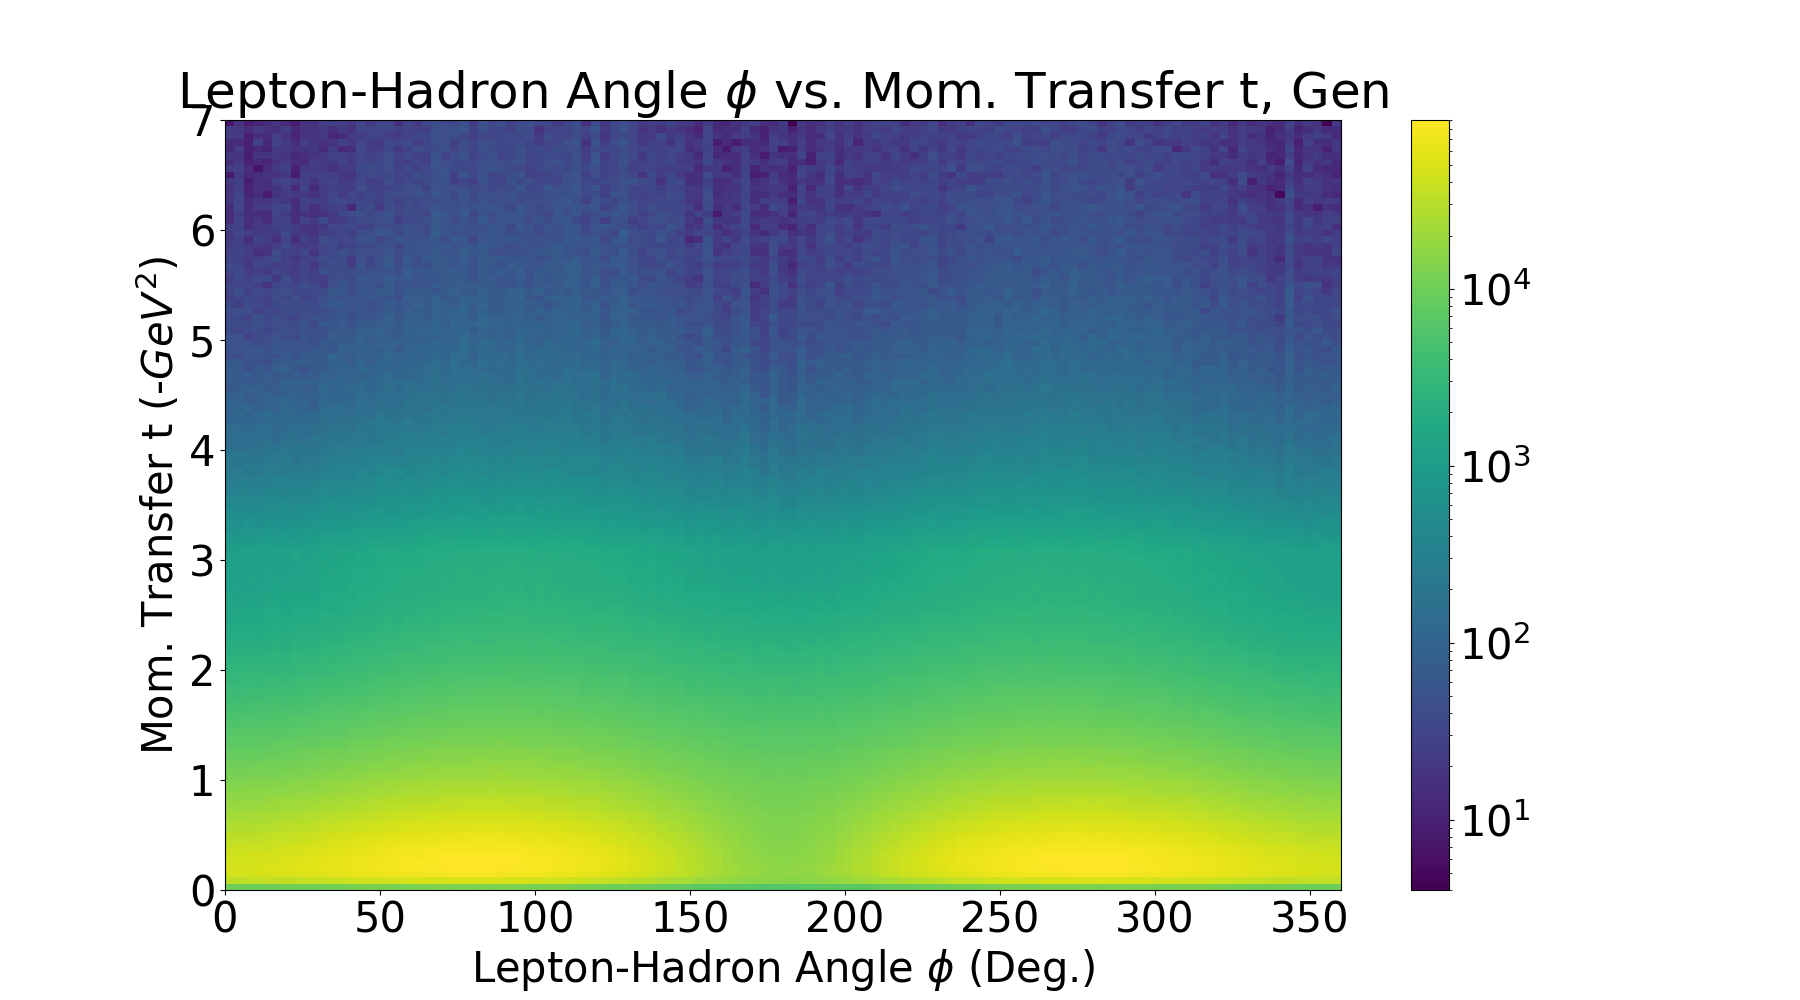
\includegraphics[width=0.5\textwidth]{Chapters/Ch3-Simulations/event_generation/pics/Lepton-Hadron_Angle_phi_vs_Mom_Transfer_t,_Gen.png}}
        \hfill
        \subfloat{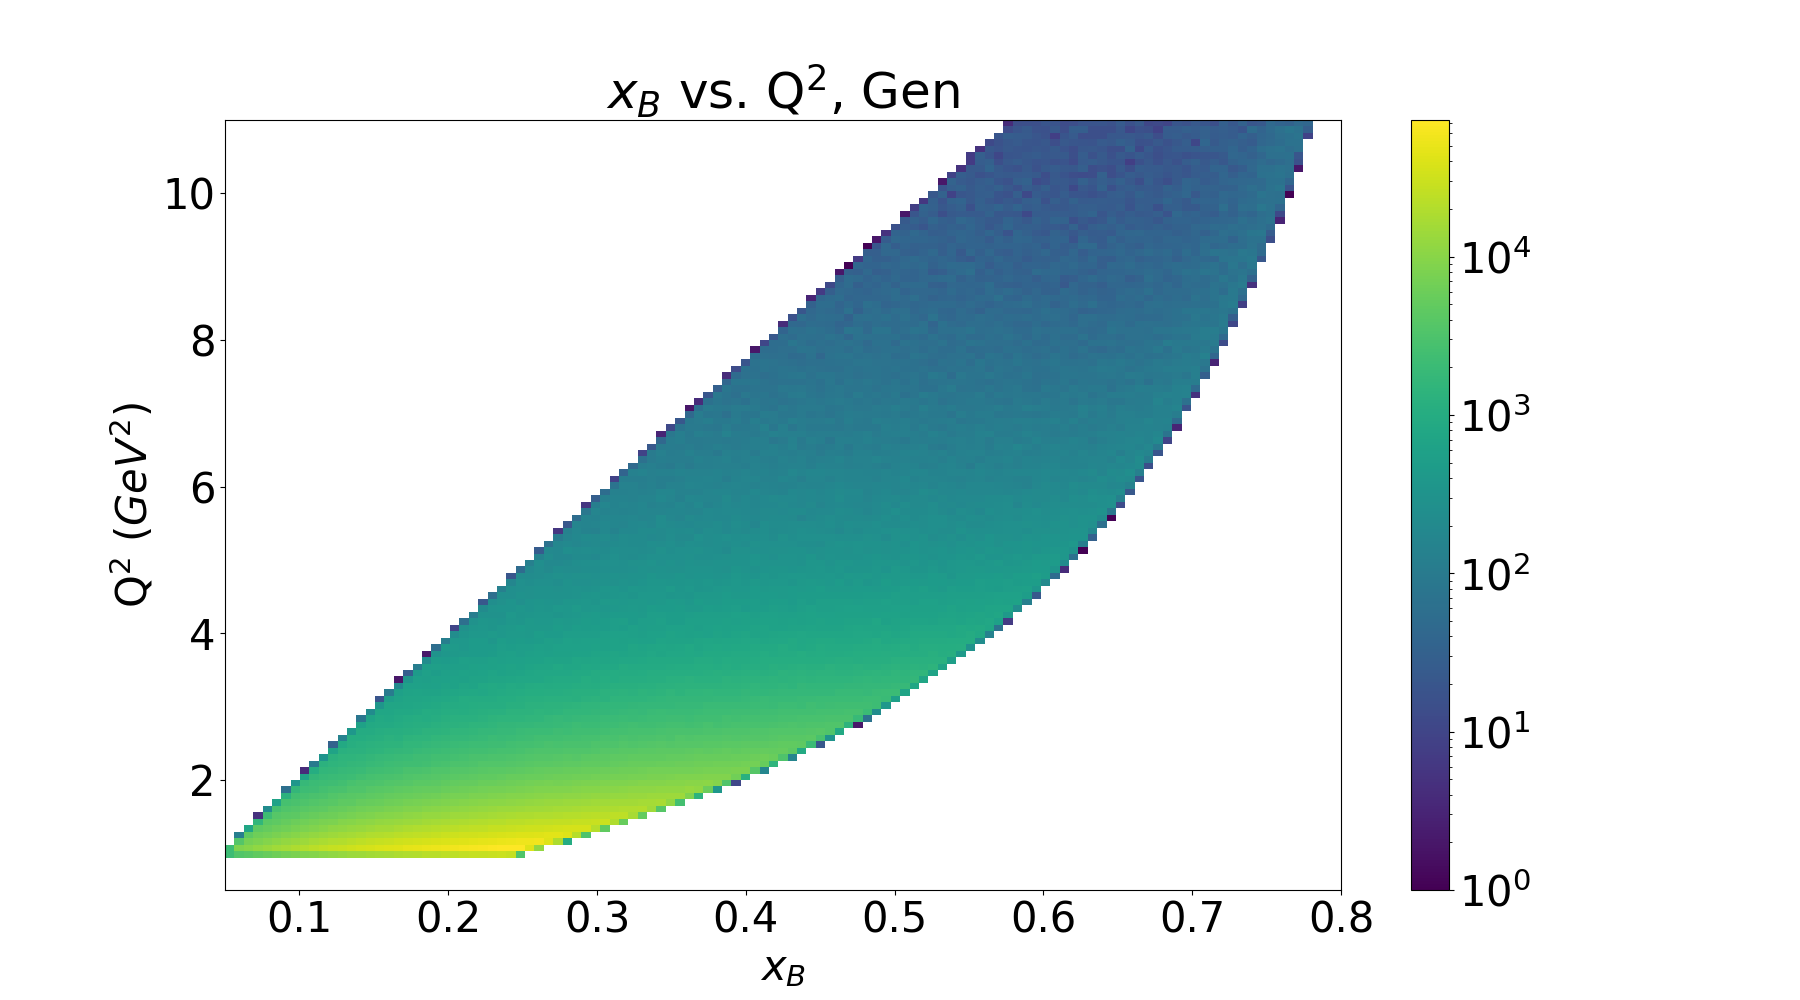
\includegraphics[width=0.5\textwidth]{Chapters/Ch3-Simulations/event_generation/pics/x_B_vs_Q2,_Gen.png}}
        \caption[Generated Event Distributions]{Generated event distributions over the 4 kinematic variables used in this work.}\label{fig:aao_norad_gen}
    \end{figure}


The radiative generator builds on the nonradiative generator to include Radiative Corrections (RC). The generator calculates s-peak and p-peak radiative corrections according to the Mo/Tsai scheme \parencite{MO1969RadiativeScattering}. The calculation produces a radiated photon with a distribution as shown in \figref{fig:aao_rad_mom_distribution}. While more realistic than the nonradiative generator, it also takes roughly 100 times as long to produce events, and so in practice both generators are utilized. 


    \begin{figure}
        \centering
        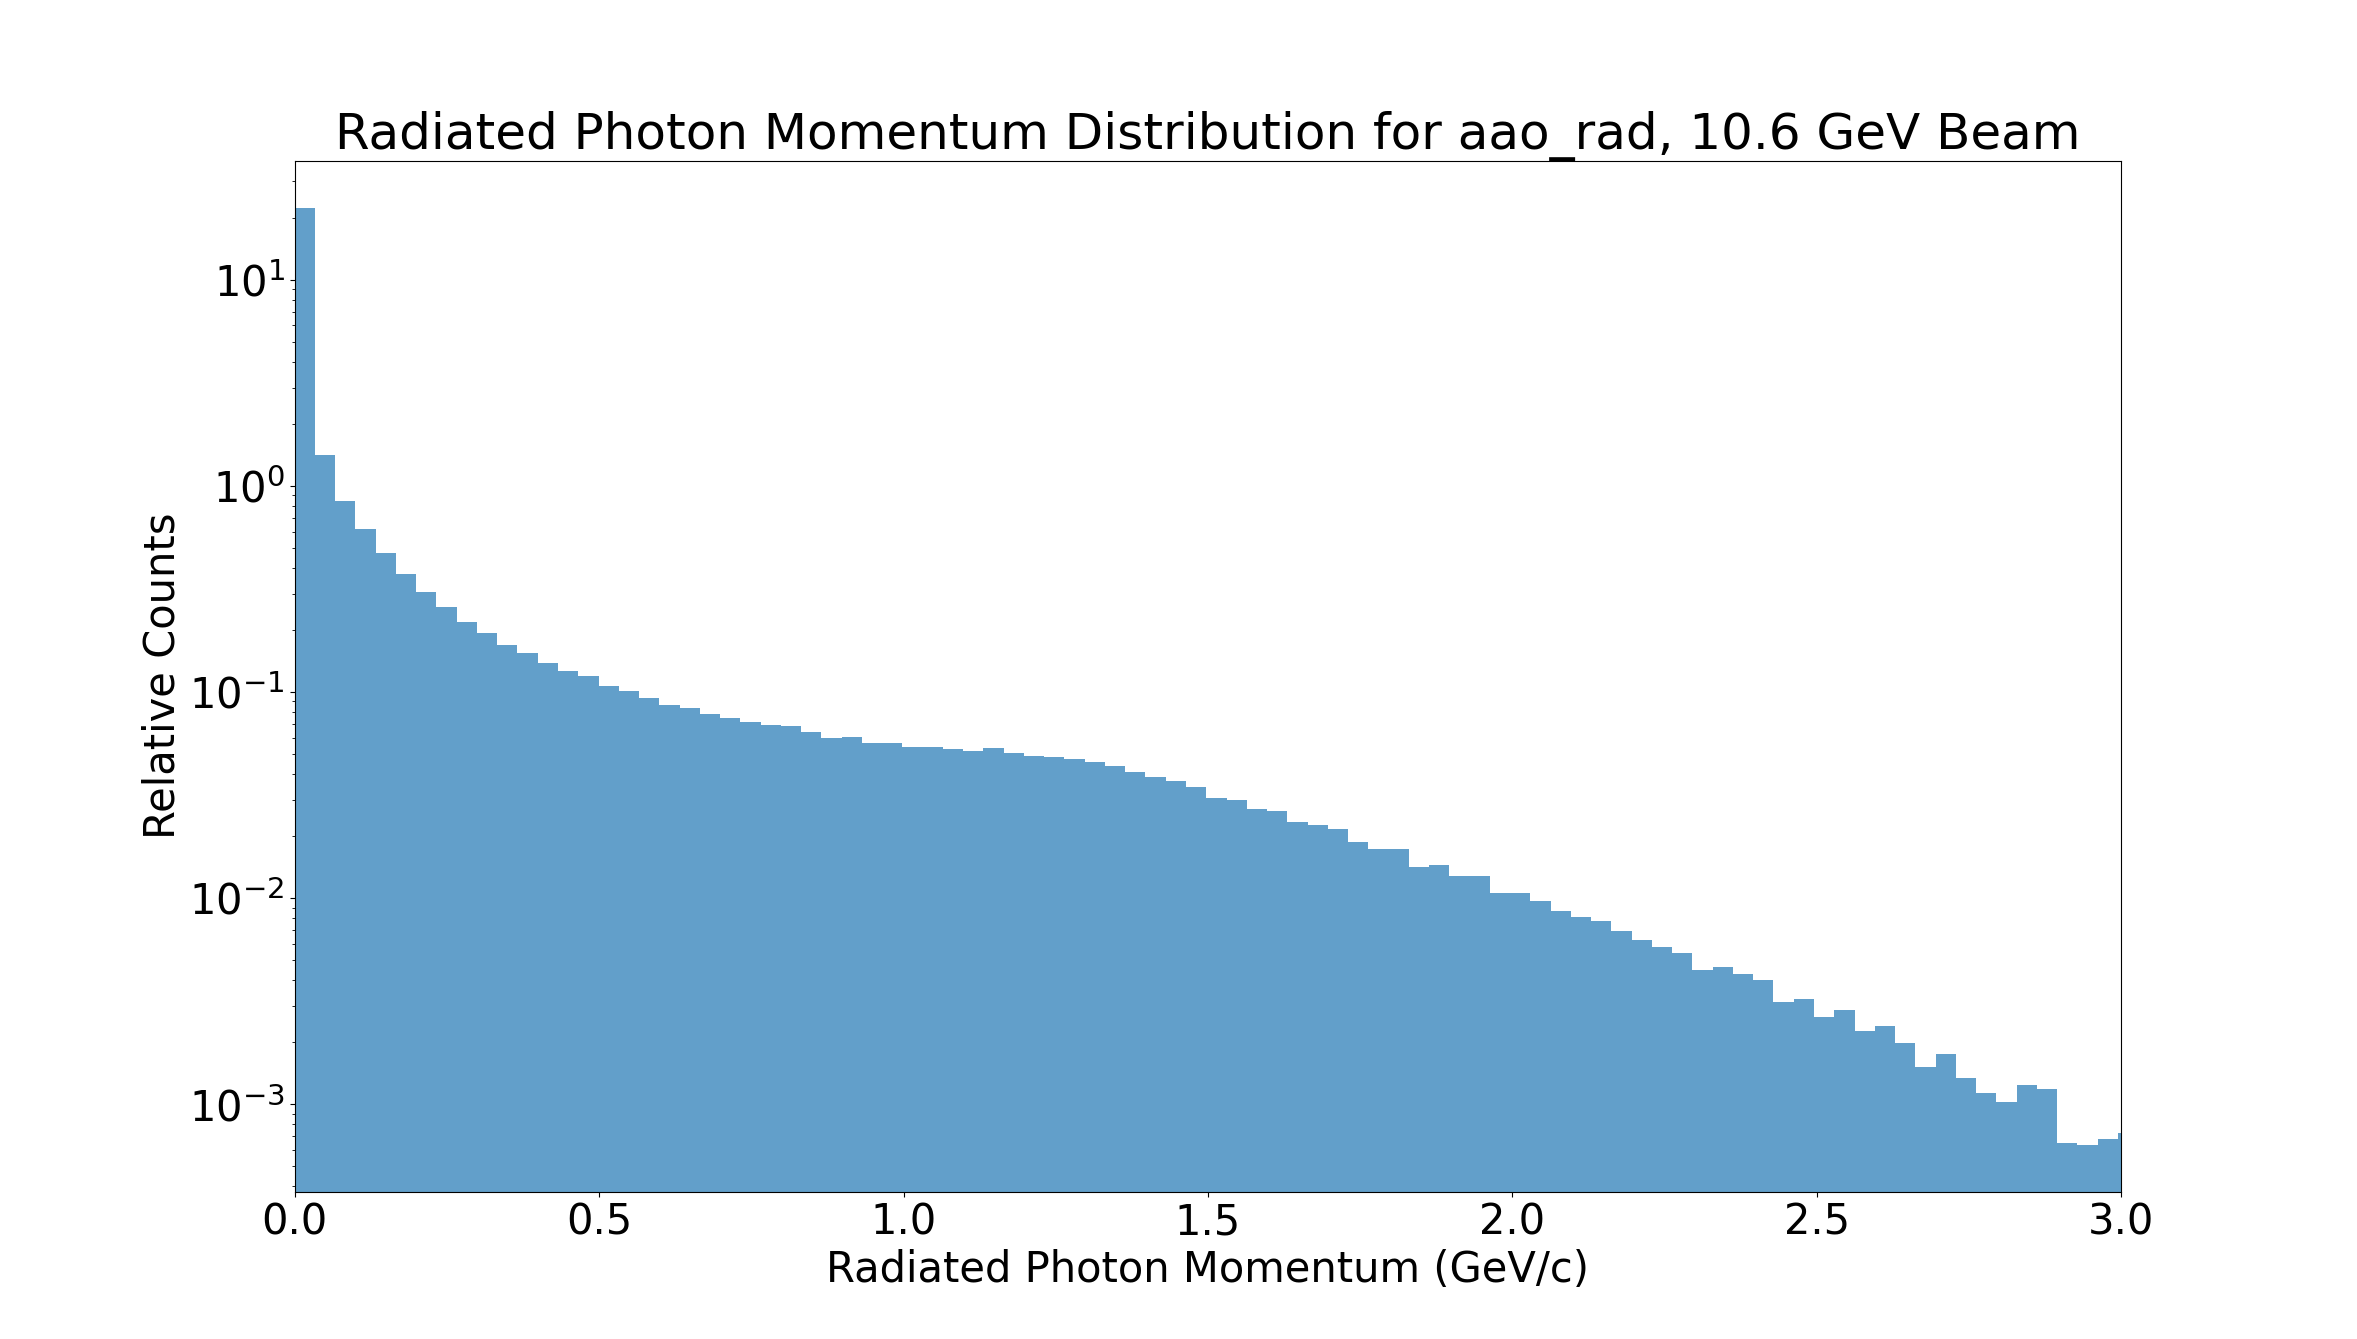
\includegraphics[trim={0 1.25cm 0 2.5cm},clip,width=0.79\textwidth]{Chapters/Ch3-Simulations/event_generation/pics/radiated_photon_momentum.png}
        \caption[aao\_rad radiated photon momentum distribution]{aao\_rad radiated photon momentum distribution. The horizontal axis is the radiated photon momentum, in units of Gev/c.}
        \label{fig:aao_rad_mom_distribution}
    \end{figure}
    
%AAO rad genreates four particles, an electron (PID 11), proton(PID 2212), radiated photon (22), and produced pion  (111)
    

%// Pi0 leptoproduction in Goloskokov-Kroll (GK) model. The code is currently being tested and implemented in PARTONS framework with additional features. If you plan to use this work in a publication, please use and reference the most recent version of PARTONS in http://partons.cea.fr 
\iffalse
% NOTES FROM VALERY KUBEROSKSKY
Andrey Kim and Nick Markov have the pi0 generator. It has my parametrization for W>2 GeV and MAID for W<1.7 GeV.

My model will for sure work for 12 GeV. It actually very close even for the COMPASS pi0 data (180 GeV muon beam).

There is reasonable coincidence between my model and MAID in the point W=1.7 GeV, not ideal but good enough for the MC.

I think actually that my parametrization has to work in the region W<2 GeV but I am not sure that MAID is doing good job due to the absence the experimental data at W~1.7 GeV. 

%FROM ONE OF THE READMES:
***************************************************************************
*      AUTHOR:        V. BURKERT AND Z. LI
*      FIRST VERSION: SUMMER, 1991.  RECENT UPDATE: MAY.1993
* AO IS WRITTEN BASED ON THE ORIGINAL PROGRAM A_AND_O FROM V.BURKERT
* THIS PROGRAM SHOULD BE LINKED TO EITHER QKMC OR QKXM FOR THE CALCULATION
* OF QUARK MODEL.  
* QKMC AND QKXM USE DIFFERENT FORM FACTORS:
* QKMC USES THE TREATMENT OF FOSTER ET. AL.
* QKXM USES THE DIPOLE FORM FACTOR 
* QKMC IS THE DEFAULT CHOICE IN THIS PACKAGE.
* AO CAN BE USED TO EXAM: Q2-DEPENDENCE OF HELICITY AMP. AT RES. POSITION (GO1)
*                         OUTPUT:GDH.TOP: A B CA(A_1/2) CB(A_3/2)
*                         GDH SUM RULE (GO2):OUTPUT GDH.TOP
*                         OBERVABLES  (RETURN):OUTPUT TEST.TOP
**************************************************************************
*           AO.FOR
* AO CONTAINS THE FOLLOWING SUBROUTINES/FUNCTIONS:
* SIGMA--CALCULATES OBSERVABLES
* EPRES--CALCULATES BREIT-WIGNER RESONANCE AMPLITUDES
* EXPA --CALCULATES THE HELICITY AMPLITUTES FROM EXPT (V.BURKERT ORIGINAL)
* BORNT--CALCULATES THE BORN TERM CONTRIBUTIONS
* BACK --CALCULATES BORN AND NON-BORN BACK GROUND TERMSS
* QKMA --CALCULATES THE HELICITY AMPLITUTES FROM QUARK MODEL
* RAMPF --CALCULATES THE Q2-DEPENDENCE OF THE HELICITY AMP. AT RES. POSITIONS
* HAMP --CALCULATES THE ENERGY-DEPENDECE OF THE RESONANCE HELICITY AMPLITUDES
* QKMC --CALCULATES THE COUPLING CONSTANTS FROM QUARK MODEL
************************************************************************
**************************************************************************
* UPDTATED: NOV., 1992
*         * WITH NEW OPTIONS TO TURN THE BORN TERM ON AND OFF
*         * BORN TERM ARE MODIFIED WITH A CUT OFF FACTOR AT HIGHER 
*           ENERGIES (WCM>1.3 GEV)
*         * SOME CORRECTIONS HAVE BEEN MADE TO THE EXPA SUBROUTINE
***************************************************************************  

 %OTHER GENERATOR NOTES:
    For Exclurad we have similar model, in end may have to iterate a few times to improve the model
    Exlclurad specifically for resonance region, theoretically should be correct, input probably needs to be updated, can put Valery’s new parameterization to cover higher range. Should not be a real issue to implement it because same thing was done for AAORad. High q2 cannot be covered because parameterization only goes to CLAS6 range
    FX: the cruicail thing is to fold in the radiative corrections with acceptance and efficiens. Best mothod is to use fast monte carlo


    aao\_rad and aao\_norad are event generators for exclusive pi0 and pi+ channels with/without radiative effects.  They are written in Fortran.  The program was initially developed by Volker Burkert long time ago for the resonance region, then has been evolved for many years and recently extended to DIS region even though lots of things need to be done.  Try this to see whether it works.  
\fi

\iffalse

    \subsection{Nonradiative Generator}
            Include generator plots, specitics of layout
    

    \subsection{Radiative Generator}
     % Include generator plots, specitics of layout, plots showing W cut offs, etc
    %SANGBAEK PG 76 RC
\fi
   
\clearpage

\section{Simulation Software}\label{sec:sim_pipeline}
 The event generators produce datafiles where each event can be thought of as being represented by four 4-vectors (corresponding to the four particles in each event). This represents the (simulated) ground truth of the event. This information must be transformed in a realistic way into the four-momenta typically observed after event reconstruction, data processing, and exclusivity cuts are applied. The most common way to achieve this result is to (1) swim each particle through a physics simulation of the CLAS12 experiment, resulting in simulated detector hits, and (2) pass the simulated detector hit data to reconstruction and analysis algorithms. 

Step (1) is realized through the use of Geomtry and Tracking (Geant4) \parencite{Agostinelli2003Geant4aToolkit}, which is a Markov-Chain Monte Carlo (MCMC) software package that simulates the microphyics at each (variable) step along a particle's path through space. This has been implemented for the CLAS12 experiment as a the ``Geant4 Monte Carlo'' (GEMC) software system \parencite{Ungaro2020TheSimulation}, which allows for the simple insertion of CAD models into the Geant4 system, with the basic architecture shown in \ref{fig:gemc_architecture}. 

\begin{figure}[htb]
    \centering
    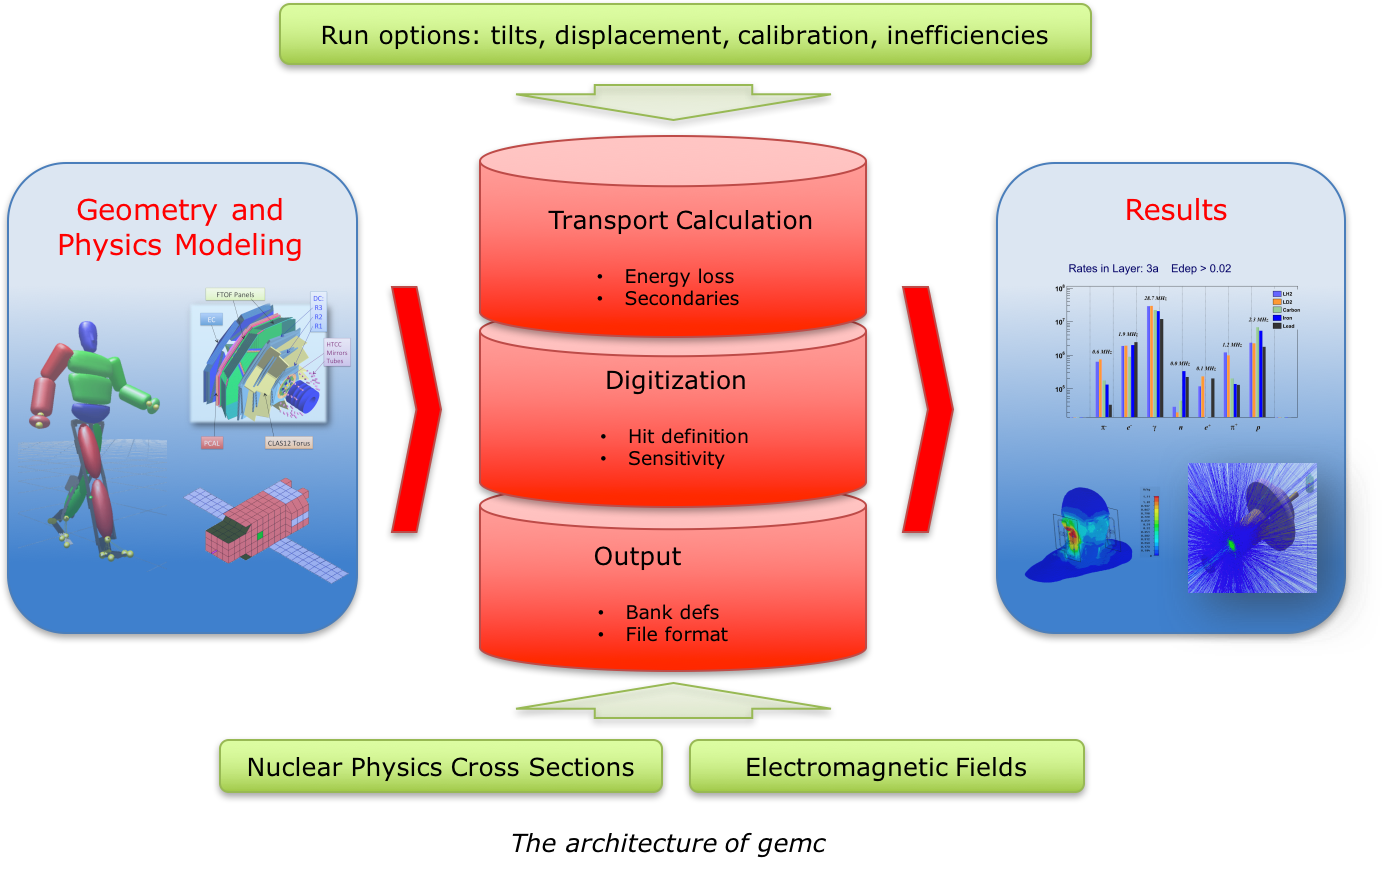
\includegraphics[width=0.65\textwidth]{Chapters/Ch3-Simulations/simulation_pipeline/pics/gemc_basics.png}
    \caption[GEMC Architecture]{GEMC architecture. Image from \parencite{Ungaro2020TheSimulation}.}
    \label{fig:gemc_architecture}
\end{figure}

Step (2) is straightforward after having been developed as discussed in \chref{Chapter:Experiment}. The distributions from \figref{fig:aao_norad_gen} after passing through the GEMC simulation, CLAS12 reconstruction software, and event selection are shown in \figref{fig:aao_norad_sim}, where the differences between the distributions is indicative of the acceptance cutoffs of the CLAS12 experiment. 


    \begin{figure}[H]
        \centering
        \subfloat[]{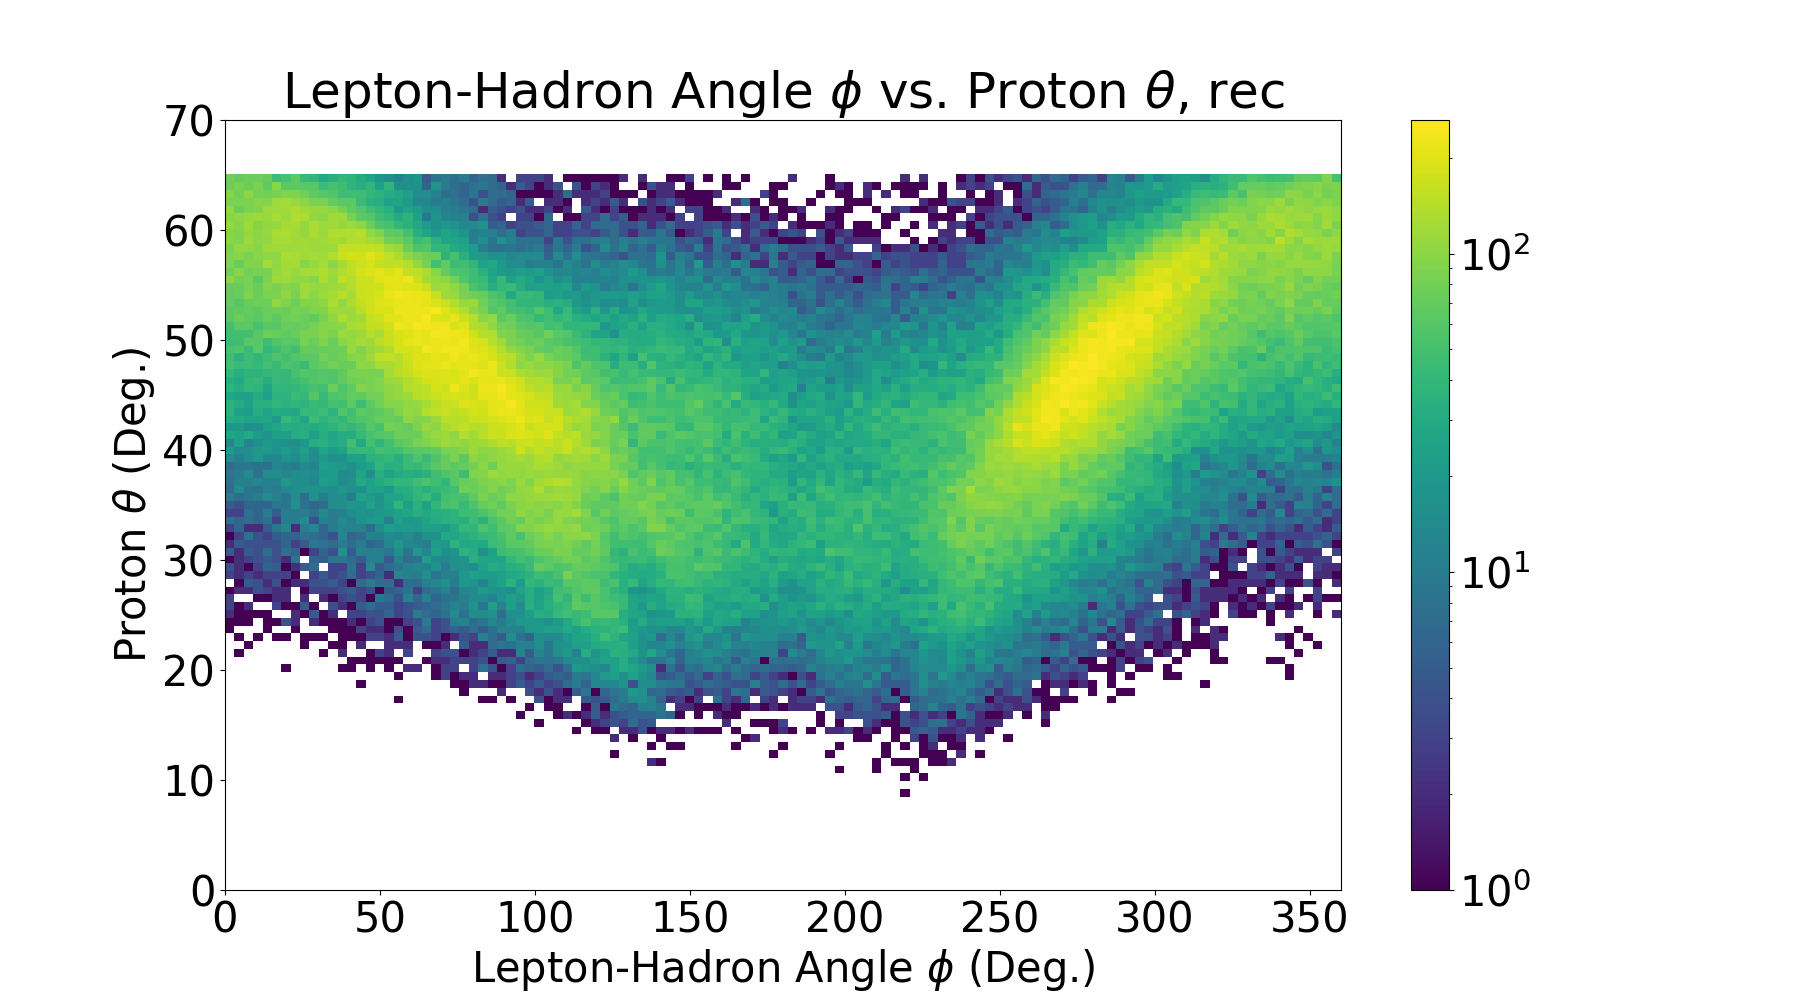
\includegraphics[width=0.5\textwidth]{Chapters/Ch3-Simulations/event_generation/pics/Lepton-Hadron_Angle_phi_vs_Proton_theta,_rec.png}}
        \hfill
        \subfloat[]{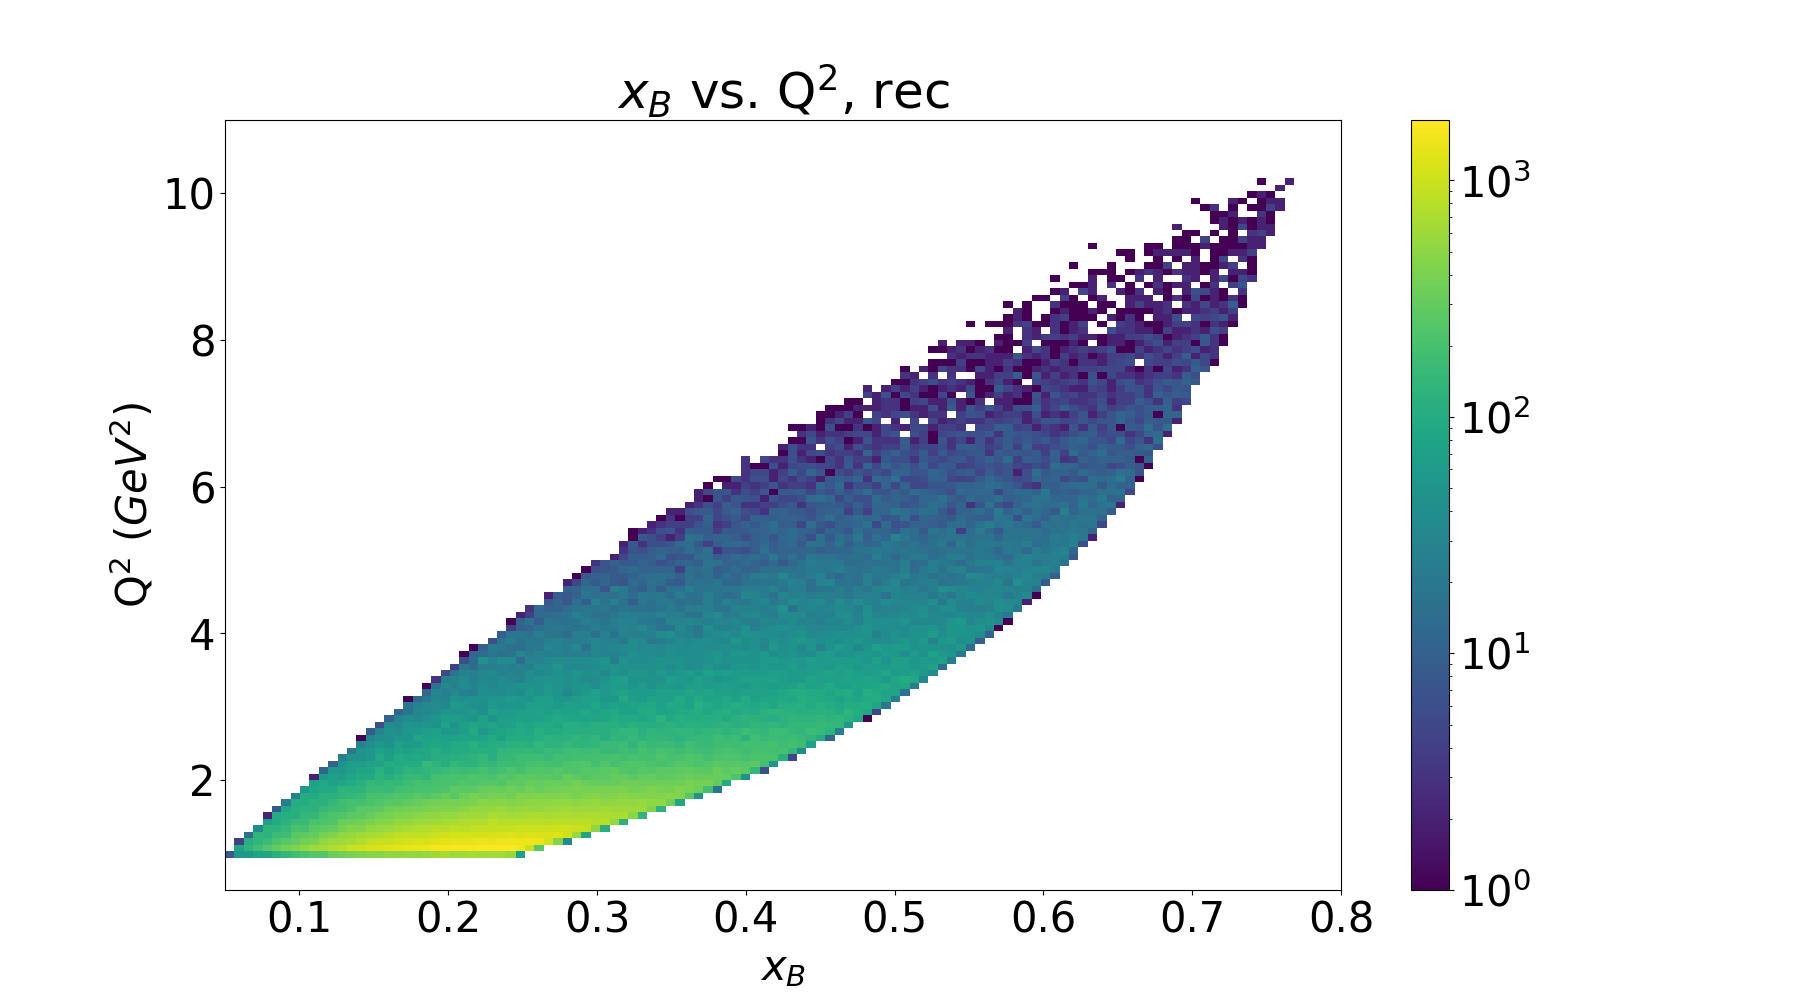
\includegraphics[width=0.5\textwidth]{Chapters/Ch3-Simulations/event_generation/pics/x_B_vs_Q2,_rec.png}}
        \caption[Reconstructed Event Distributions]{Reconstructed event distributions}\label{fig:aao_norad_sim}
    \end{figure}

\iffalse
    
    Event generation - fortran and c++ python wrapped
    geant4 docker gemc sysem
    reconstruction from part 2
    
    CLAASana
    
    this should talk about Geant4, GEMC, microphysics MCMC

\fi


    
        



\section{Computational Resources and Infrastructure}\label{sec:comp_infrastructure}
   
    Generating realistic \dvpip events and simulating physics experiments are computationally intensive tasks. Personal computers can run the necessary software, but a sufficient number of simulated events would require an unacceptably long amount of time on a single device. Consequently, much effort has been devoted to the construction of computational centers and corresponding data pipelines to facilitate large scale computing efforts. 

\subsection{Scope of Computations}

    How many simulated events are needed? The simple answer is ``many''. As the number of simulated events grows, the uncertainty of the acceptance estimator $\hat{\epsilon}_{acc}$ (and other computationally derived correction factors) decreases. While simulated data are significantly less expensive than experimental data, they are not free and therefore some realistic bound must be made. As a quick heuristic, it is reasonable to perform enough simulations so as that the uncertainty of the $\hat{\epsilon}_{acc}$ is negligible compared with the other uncertainties of the measurement, or at least is non-dominant. Considering only the acceptance correction in the cross section, \eqref{eq:DVPiPCrossSection_acc_corr}

    
     \begin{equation}\labelAndRemember{eq:DVPiPCrossSection_acc_corr}
           { \frac{    d^4\sigma_{  ep \rightarrow ep'\pi^0}   } {dQ^2dx_Bdtd\phi_{\pi}} 
                =   \frac{ \textcolor{red}{ N(Q^2,x_B,t,\phi_{\pi})}} {\Lumiint \textcolor{purple}{ \Delta \Omega}}
                \frac{1}{\textcolor{correctionfactors}{\epsilon_{acc}}} \approx \frac{ \textcolor{red}{ N_{exp} }} {\Lumiint \textcolor{purple}{ \Delta \Omega}}  \frac{\textcolor{correctionfactors}{N_{gen}}}{\textcolor{correctionfactors}{N_{sim}}}},
     \end{equation}     

     we have the statistical uncertainty from the experimental and stimulated number of events as \eqref{eq:uncert_sum}

    \begin{equation}\label{eq:uncert_sum}
               { 
               \frac{\delta_{\sigma}}{\sigma} = \sqrt{
                \left(\frac{\delta_{N_{exp}}}{N_{exp}} \right)^2+
                \left(\frac{\delta_{N_{sim}}}{N_{sim}} \right)^2 }               }.
         \end{equation}

    %Note that this equation only discusses the uncertainties due to Nsim Nexp for illustration

    The uncertainty in N$_{exp}$ and N$_{sim}$, $\delta_{N_{exp}}$ and $\delta_{N_{sim}}$ respectively, are given by $\sqrt{N_{exp}}$ and $\sqrt{N_{sim}}$, which assumes applicability of a Poisson distribution to the process, commonly known as ``counting statistics'' further discussed in \parencite{Knoll2000RadiationMeasurement}. We can then consider the effect of setting \Nsim = X\Nexp, where X is some multiplicative factor. The expression for the total uncertainty then can be reduced to \eqref{eq:uncert_sum_reduced}

        \begin{equation}\label{eq:uncert_sum_reduced}
               {\frac{\delta_{\sigma}}{\sigma} = \sqrt{ \left( \frac{ \sqrt{ N_{exp}} } { N_{exp}} \right)^2  +  \left( \frac{ \sqrt{ X N_{exp}} } { X N_{exp}} \right)^2     } =  \left(\frac{\delta_{N_{exp}}}{N_{exp}} \right) \sqrt{ \left(1+\frac{1}{X} \right)}}.
        \end{equation} \myequations{Relationship between \Nsim and statistical uncertainty}

    The relationship between the combined statistical uncertainty and the number of simulated datapoints is displayed graphically in \figref{fig:simulation_stats_increase}. Other uncertainties in this measurement are at the 5\%-10\% level (\secref{sec:Ch4_corr_factors}) so a reasonable first-pass goal targets the statistical uncertainty due to simulation to sit at the 5\% level, corresponding to a factor X = 10 times more simulated events than experimental events. 
    
    \begin{figure}[htb]
        \centering
        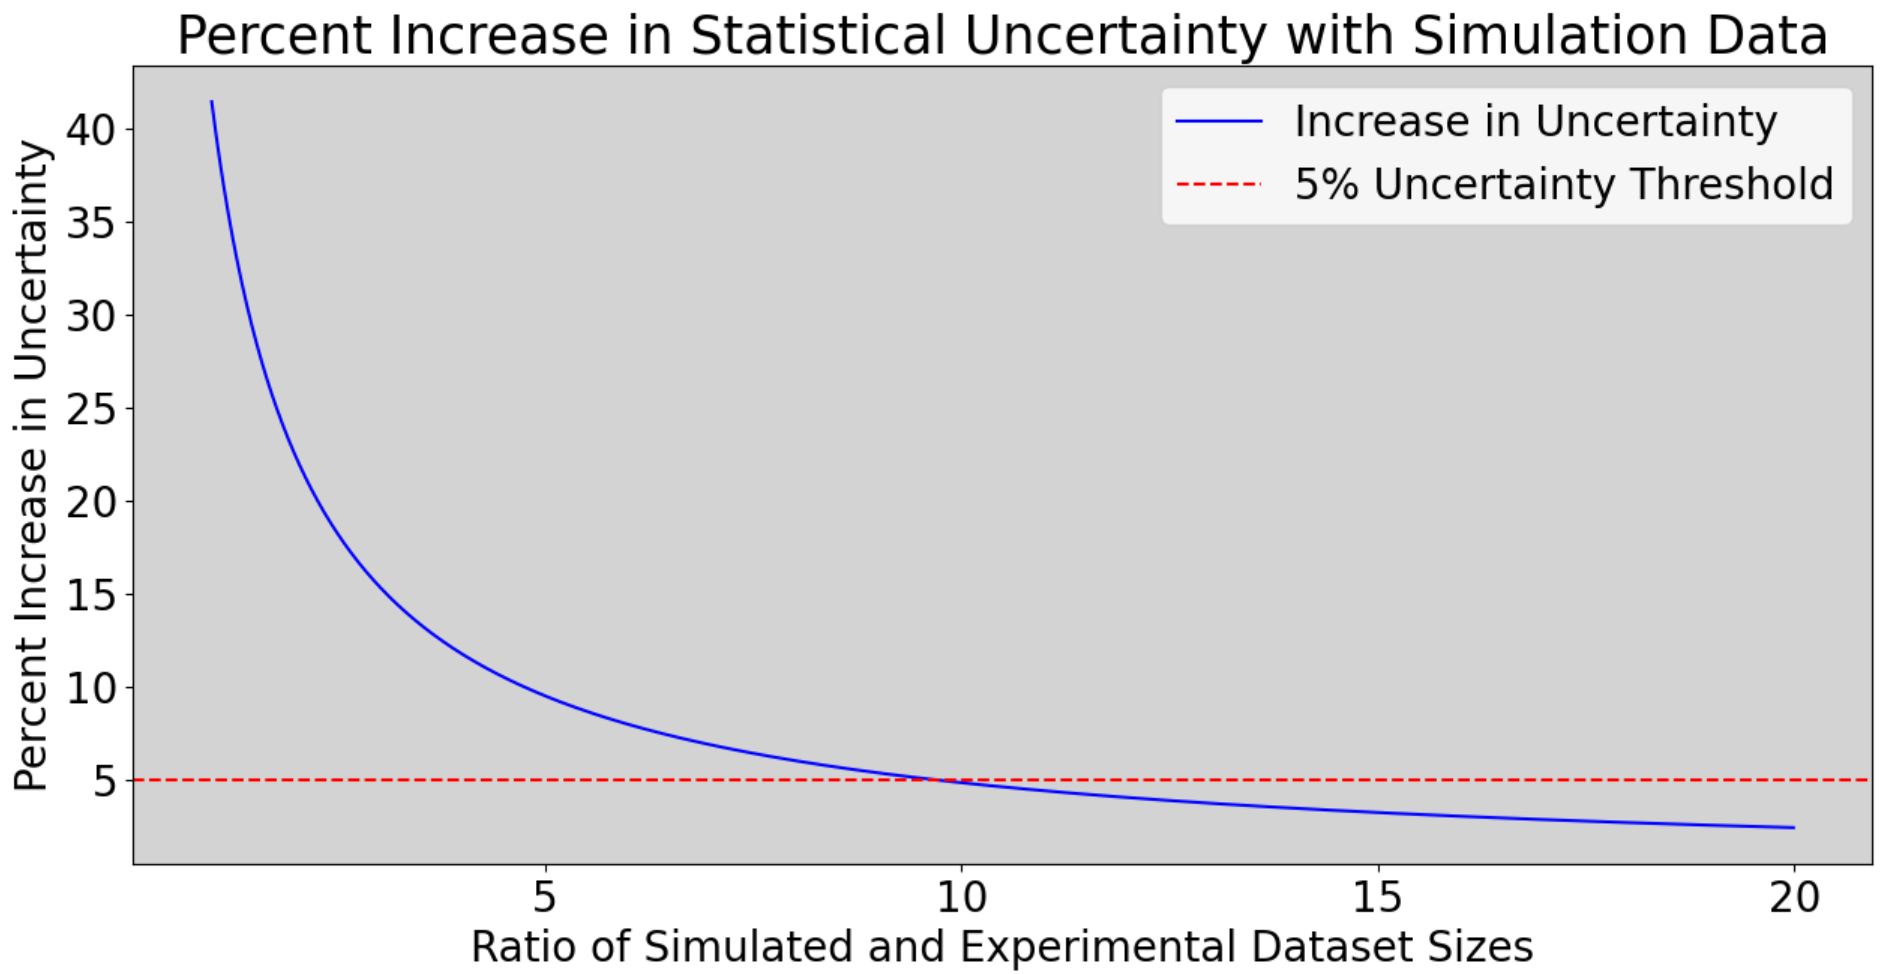
\includegraphics[width=0.8\textwidth]{Chapters/Ch3-Simulations/overview/pics/uncertainty_increase_rectangle.png}
        \caption[Comparison between Experimental and Statistical Counting Uncertainties]{Ratio of magnitudes of statistical uncertainties associated with N$_{sim}$ and N$_{exp}$ as a function of X = $\frac{N_{sim}}{N_{exp}}$. See \appref{app:f} for more details.}
        \label{fig:simulation_stats_increase}
    \end{figure}

    Preliminary analysis revealed that the total number of \dvpip events from the experimental datasets considered was approximately 500,000 ($\sim$ 200,000 from the inbending configuration, 300,000 from the outbending configuration). This corresponds to requiring $\sim$ 5 million simulated events (passing all levels of reconstruction and exclusivity cuts). The acceptance correction factor was expected to be on the order of 1/20 - 1/100, suggesting the need for several hundred million generated events to be passed through the simulation pipeline. \tabref{table:Generated_Data} displays the simulation allocation scheme implemented in this analysis, with higher statistics assigned to the nominal experiment running parameters, and additional simulations budgeted for variational studies and correction factor determination, as further discussed in \chref{Chapter:BaseAnalysis}.


    \iffalse
    \begin{table}[h]
        \centering
        \begin{tabular}{l|lccc}
            \textbf{Config.} & \textbf{Gen. Type} & \textbf{Background} & \textbf{Nevents (MM)} & \textbf{Purpose} \\ \hline
                & norad & none & 100 & Ineff. Study \\
                & norad & 50 nA & 100 & Ineff. Study / Rad. Corr \\
            In. & rad & 50 nA & 300 & Acceptance Corr. \\
                & rad & 45 nA & 100 & Systematics \\
                & rad & 55 nA & 100 & Systematics \\ \hline
                & norad & none & 100 & Ineff. Study \\
                & norad &  50 nA & 100 & Ineff. Study / Rad. Corr \\
            Out. & rad & 50 nA & 300 & Acceptance Corr. \\
                 & rad & 40 nA & 100 & Systematics \\
             & rad & 40 nA (+1.01) & 100 & Systematics \\
            \hline
            Total & - & - & 1400 & - \\
        \end{tabular}
    \caption{Data for various experimental configurations and conditions.}
    \label{table:experiments}
    \end{table}
    
    \fi
    

    \begin{table}[htb]
        \centering
        \begin{tabular}{c|ccc}
            \textbf{Configuration} & \textbf{Gen. Type} & \textbf{Background} & \textbf{Nevents (MM)} \\ \hline
                & norad & none & 100 \\
                & norad & 50 nA & 300 \\
            Inbending & rad & 50 nA & 300 \\
                & norad & 45 nA & 100 \\
                & norad & 55 nA & 100 \\ \hline
                & norad & none & 100 \\
                & norad &  50 nA & 300 \\
            Outbending & rad & 50 nA & 300 \\
                 & norad & 40 nA & 100 \\
             & norad & 40 nA (+1.01) & 100 \\
            \hline
            Total & - & - & 1800 \\
        \end{tabular}
    \caption[Distribution of Generated Events by Configuration]{Number of events generated for various experimental configurations and conditions.} %\tabref{table:simulated_data} shows this distribution after simulation, reconstruction, and exclusivity cuts.}
    \label{table:Generated_Data}
    \end{table}


    Optimization studies showed that the most computationally efficient batching scheme was to process batches of 10K events to GEMC at a time, which was the bottleneck in the simulation pipeline at 4.5 - 5 hours per job. The non-radiative (radiative) event generator requires 10 minutes (100 minutes) to produce 10K events, and further processing upon completion of GEMC requires $\sim$ 10 minutes per 10K events. This totals $\sim$ 5 hours (6 hours) per 10K events, corresponding to nearly 1 million core-hours for the required total number of simulations, which would take 8 years of continuous running on a single, high-end, 16 core computer. Instead, computing clusters at MIT, JLab, and around the globe were utilized to realize these computational efforts in a much more reasonable timeframe. 
    









    
    \todo{find some way to include the distribution of ambient radiation (cememnt, etc) - Knoll 767 -  into thesis appendix - include discussion of background merging - not an issue at these scales}


\subsection{MIT Tier 2 and High Throughput Computing}

    The primary computing center utilized for this analysis effort was the MIT Tier 2 cluster, located at the MIT Bates Research and Engineering Center in Middleton, MA, which has 1,088 cores dedicated to CLAS12 computing \figref{fig:BatesComputing}.  Also used for this work was the Massachusetts Green High Performance Computing Center (\href{https://www.mghpcc.org/}{MGHPCC}) in Holyoke, MA. MIT Earth and Planetary Science provides access to these nodes through their \href{https://engaging-ood.mit.edu/pun/sys/dashboard}{Engaging} system, while the MIT Tier 2 cluster is accessible via the \href{https://submit.mit.edu/}{subMIT} system, which also grants users access to a number of other (non-dedicated) computing clusters.

    


    %1,088 cores dedicated to CLAS computing. I believe this means we have 24 hours per day * 1088 cores = ~ 26K core hours per day dedicated   
    %The Bates Laboratory center consists of 71 water-cooled racks, each of which can supply up to 12 kW of power and cooling, and a high-speed 100 Gb/s network link to campus. It uses about 500 kW of power to operate and have 20 petabytes of storage at present.


    \begin{figure}
        \centering
        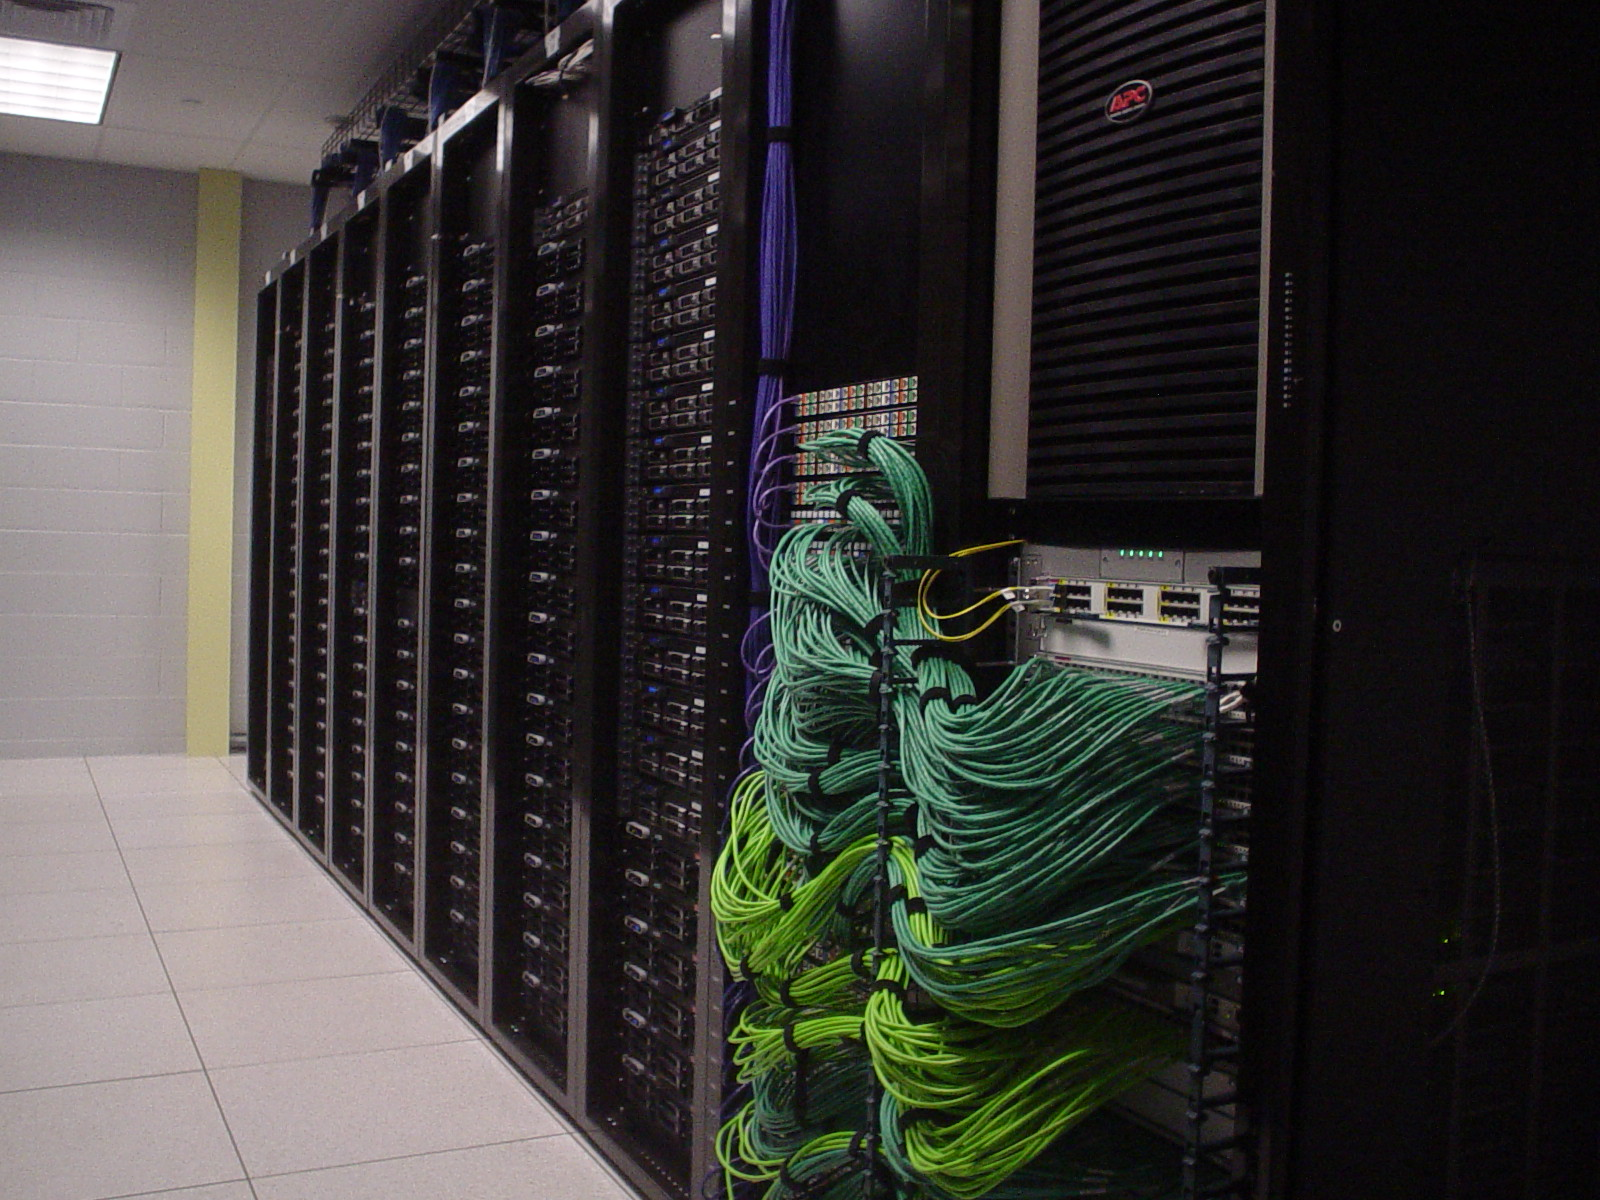
\includegraphics[width=0.8\textwidth]{Chapters/Ch3-Simulations/overview/pics/Bates_Tier2.jpg}
        \caption[MIT Tier 2]{MIT Tier 2 computing racks at MIT Bates. Image courtesy of E. Ihloff}
        \label{fig:BatesComputing}
    \end{figure}


    
    %and is, which is a larger computational framework that additionally provides access to other computing centers,



    %SUBMIT:     1 TB of free storage per user,     100s of cores and GPUs available interactively and through Slurm     Access to OSG, CMS T3 and T2, LQCD Cluster, and EAPS


    More broadly, the Open Science Grid (OSG) \parencite{OSG2006OSG} \parencite{Sfiligoi2009TheGlideinWMS} \parencite{Pordes2007TheGrid} was leveraged to gain access to dozens of computing clusters around the world. OSG is an organizational system allowing users to utilize idling resources at more than 100 participating institutions, facilitating more than a billion core-hours of computation per year. 

    A significant endeavor in this work was constructing a software bridge connecting the CLAS12 experiment and these computing resources. The effort was realized as the \href{https://gemc.jlab.org/web_interface/index.php}{CLAS12 Simulation Submission Portal} \parencite{Ungaro2020CLAS12Framework}, which established the database back-end, user-friendly front-end \figref{fig:clas12_sub_portal}, and appropriate connection services to interact efficiently with these clusters. 
      
    \begin{figure}[H]
        \centering
        \newlength{\imageheight}
        \settoheight{\imageheight}{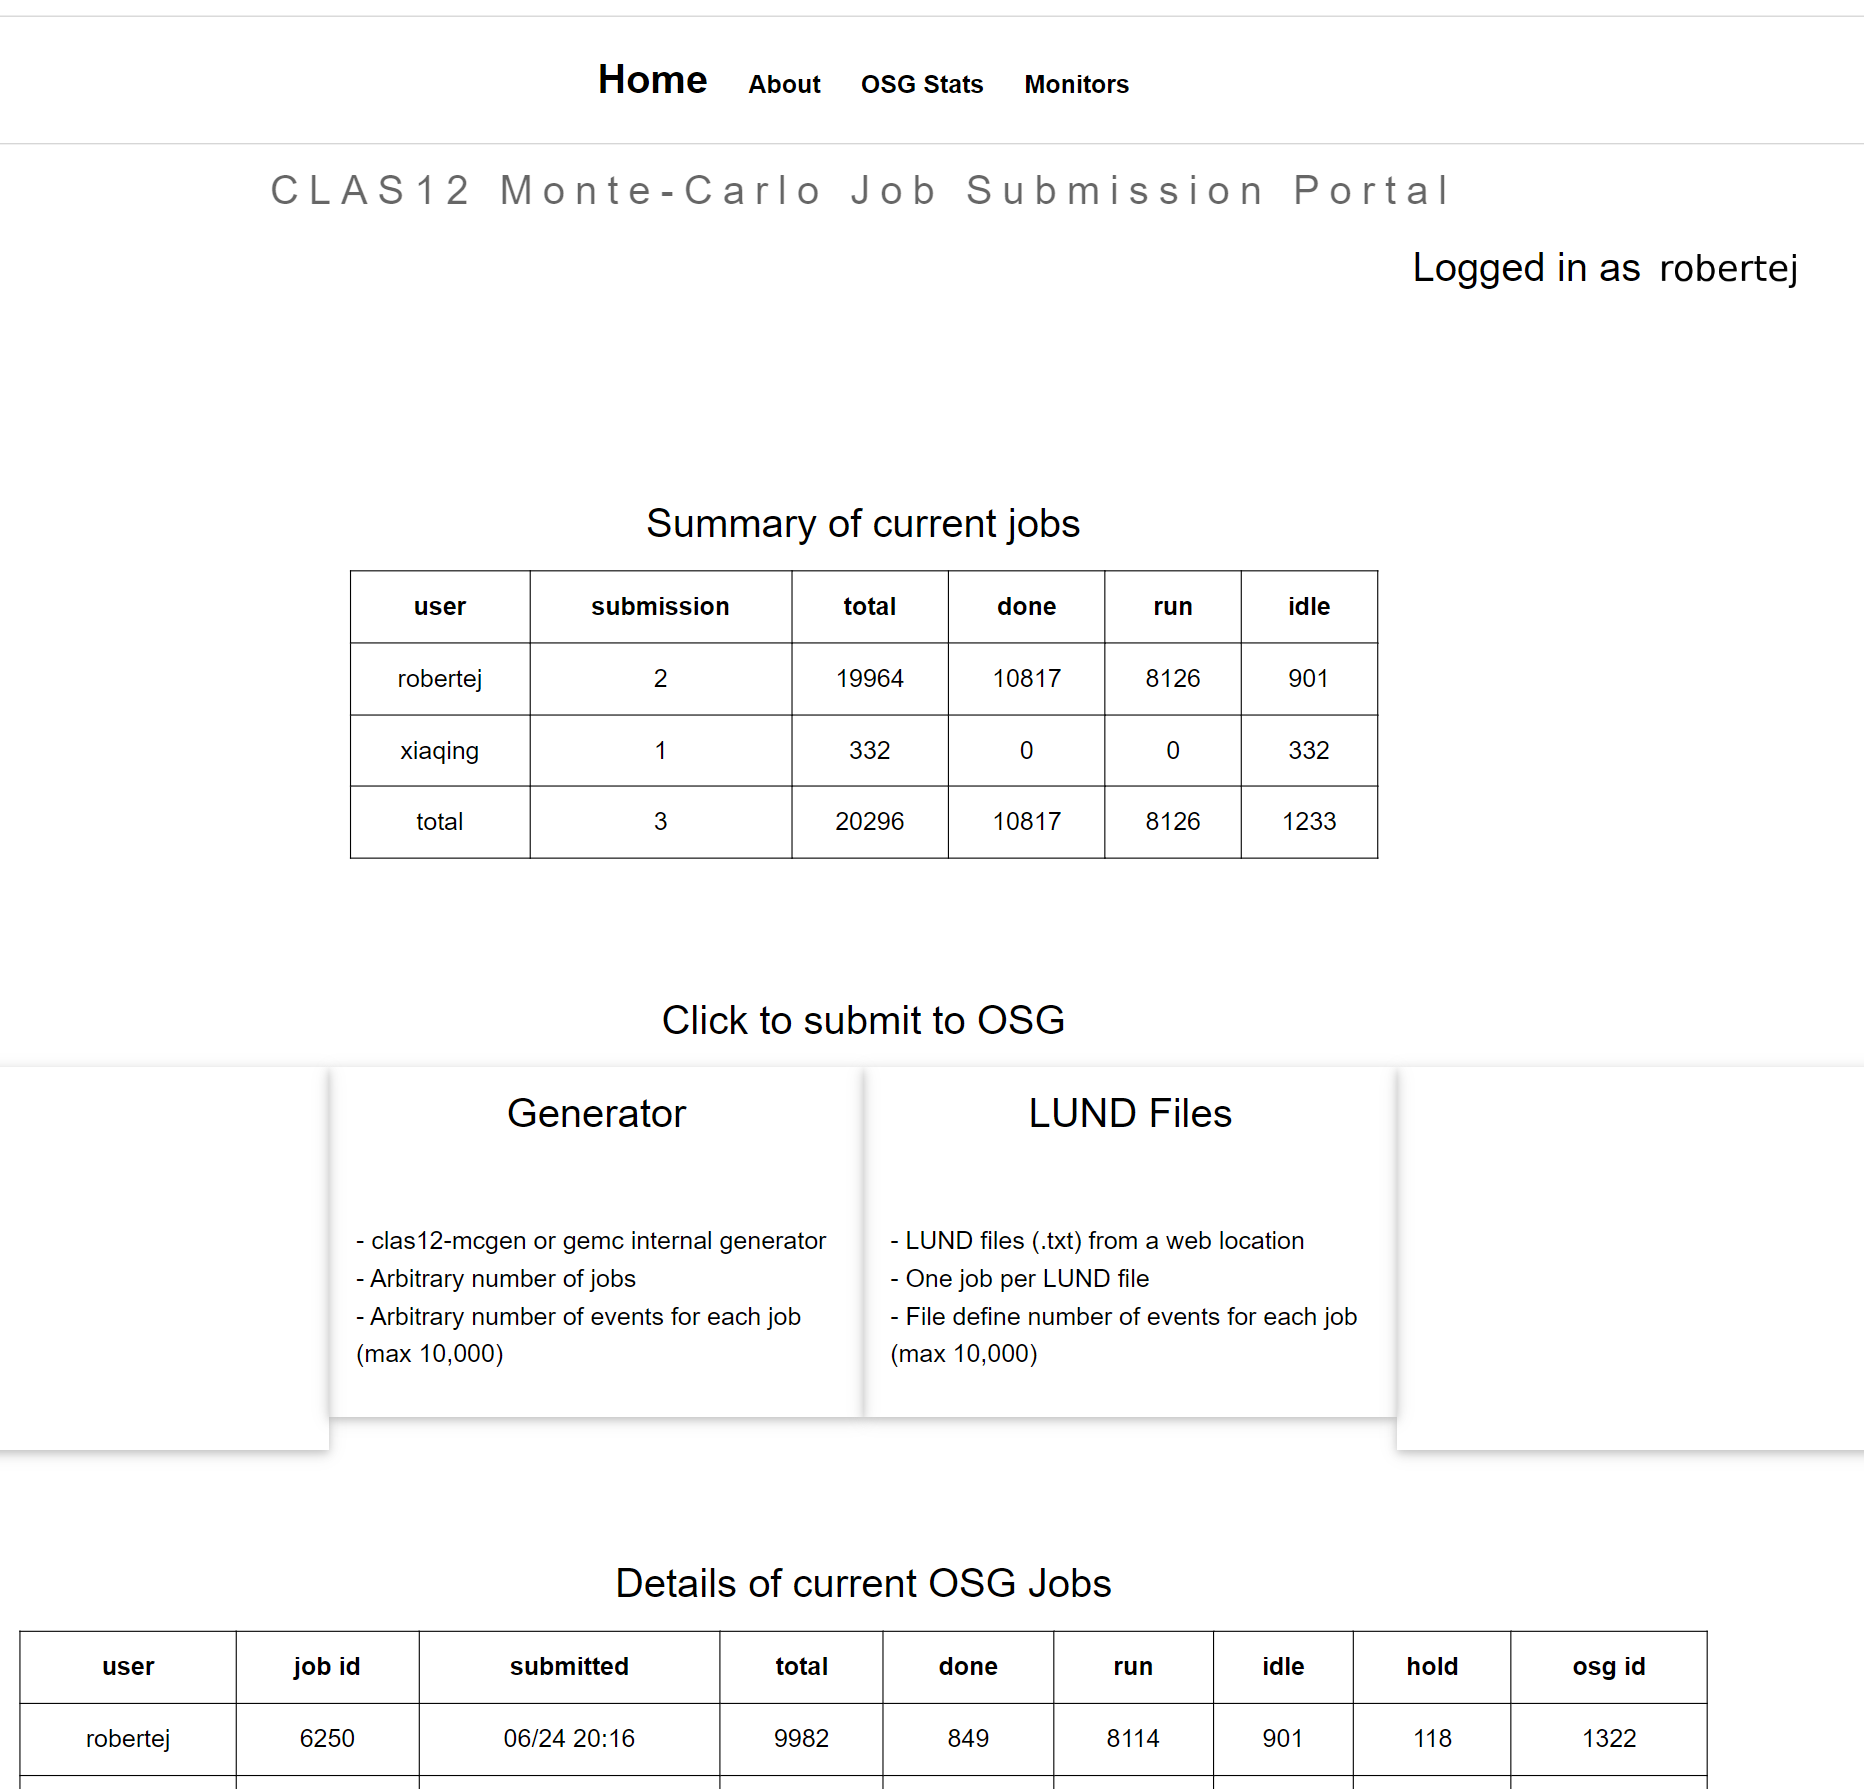
\includegraphics[width=0.5\textwidth]{Chapters/Ch3-Simulations/overview/pics/websub_start_narrow_new.png}}
        \subfloat[CLAS12 Submission Portal Main Page]{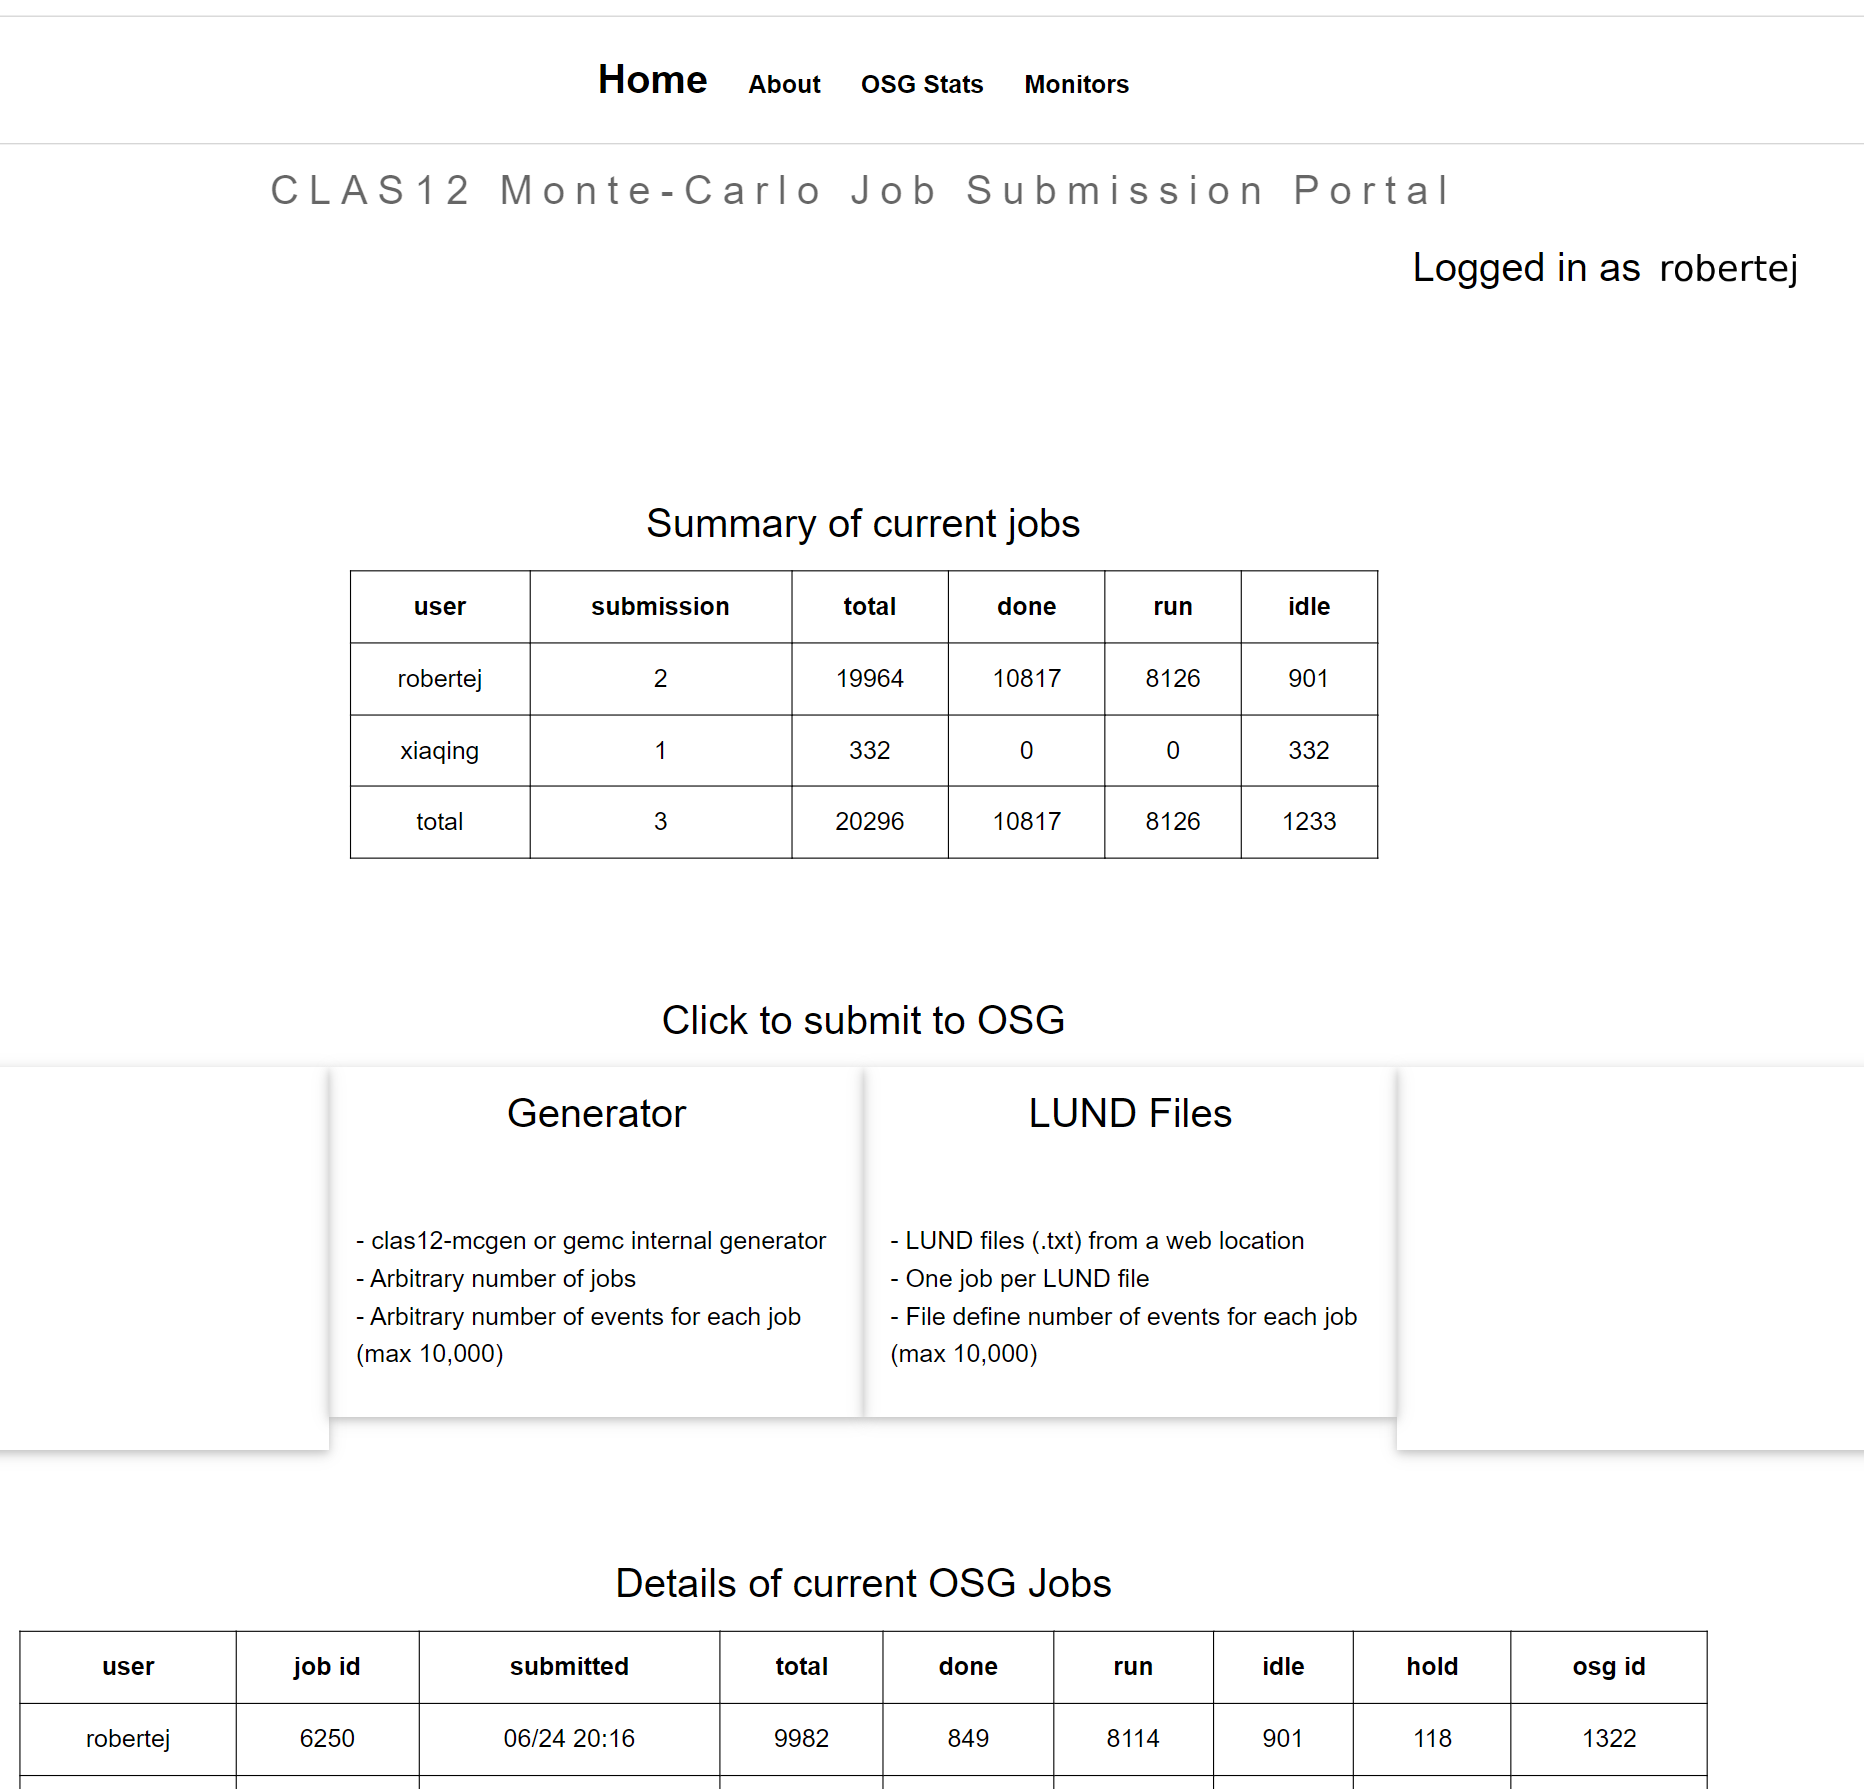
\includegraphics[width=0.5\textwidth]{Chapters/Ch3-Simulations/overview/pics/websub_start_narrow_new.png}}
        \hfill
        \subfloat[Simulation Sample Webform]{\raisebox{\dimexpr\imageheight-\height}{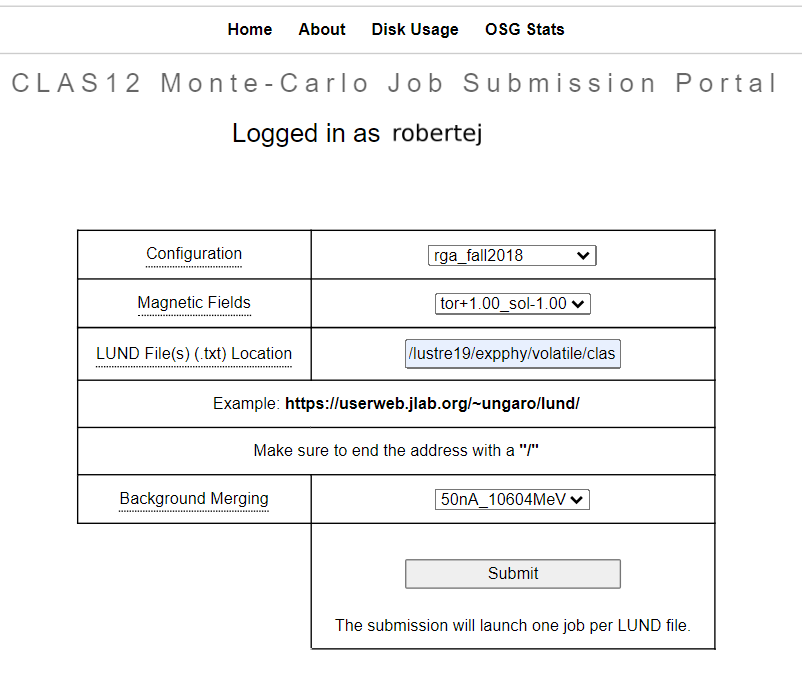
\includegraphics[width=0.45\textwidth]{Chapters/Ch3-Simulations/overview/pics/websub_lund.png}}}
        \caption[CLAS12 Simulation Submission Portal]{The CLAS12 Simulation Submission Portal, designed to facilitate efficient high-throughput simulations using a variety of generators and experimental configurations.}\label{fig:clas12_sub_portal}
    \end{figure}

    The system is capable of using any event generator on the CLAS collaboration list of \href{https://github.com/JeffersonLab/clas12-mcgen}{officially approved generators} or by passing any internet-accessible folder location of generated event files conforming to the \href{https://gemc.jlab.org/gemc/html/documentation/generator/lund.html}{LUND} standard. As of July 2023, the aao\_gen generators were not yet recognized as officially supported, so event generation had to occur independently of this system, although work is ongoing to recieve offical status. Inferfacing with computing nodes is facilitated through use of Simple Linux Utility for Resource Management (SLURM) \parencite{Yoo2003SLURM:Management} and High Throughput Computing - HTCondor \parencite{HTCondorTeam2023HTCondor} protocols. The system has been succesful, facilitating 85.2 million core-hours of CLAS12 simulations over 2021-2022 as shown in \figref{fig:monthly_hours}.
       
    
    \begin{figure}
        \centering
        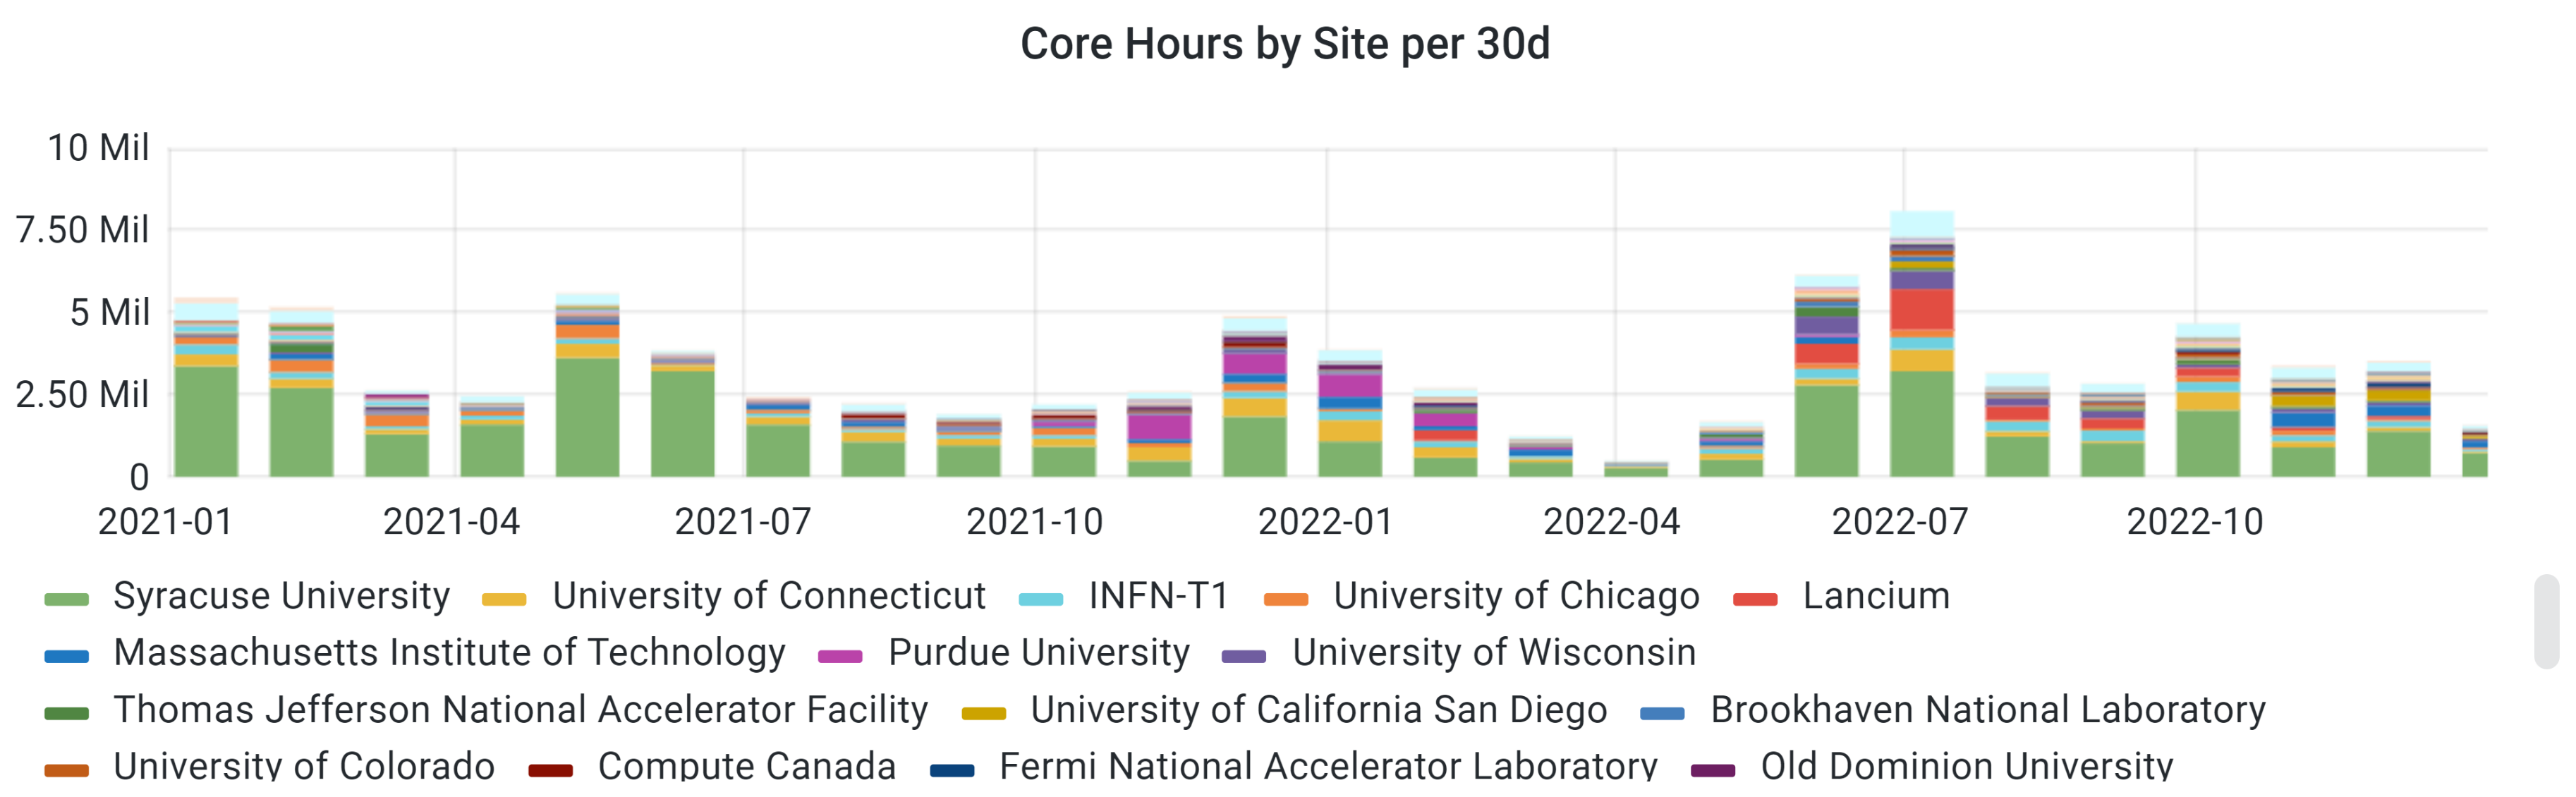
\includegraphics[width=0.99\textwidth]{Chapters/Ch3-Simulations/overview/pics/core_hours_2021-22.png}
        \caption[Monthly Core-Hours Utilized at Various Computing Clusters]{Monthly core-hours used for CLAS12 simulations in 2021-22. The portal facilitated 85.2 million core-hours of simulations over the past 2 years.}
        \label{fig:monthly_hours}
    \end{figure}

    Finally, files can be transferred easily from computing clusters to local/personal machines through the use of \href{https://www.globus.org/}{Globus} \parencite{Allen2012SoftwareScientists} \parencite{Foster2011GlobusServices}, or directly through use of ssh protocols. The complete data pipeline for simulations used in this analysis is shown in \figref{fig:simulation_workflow}.


    \begin{figure}
        \centering
        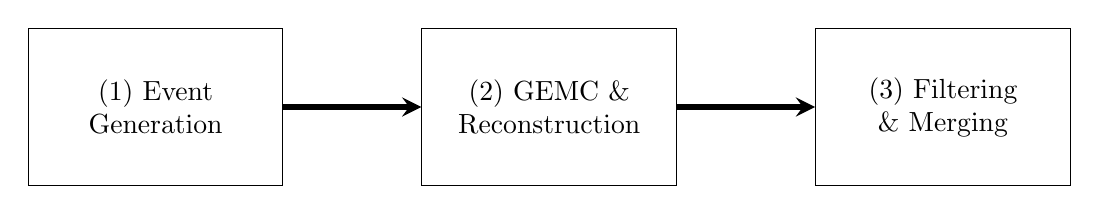
\begin{tikzpicture}[
            box/.style={rectangle, draw, minimum size=2cm, text width=3cm, align=center},
            arrow/.style={->, >=stealth, line width=2pt},
        ]
        
        \node[box] (event) at (0,0) {(1) Event \\ Generation};
        \node[box] (gemc) at (5,0) {(2) GEMC \& \\ Reconstruction};
        \node[box] (filter) at (10,0) {(3) Filtering \& Merging};
        
        \draw[arrow] (event) -- (gemc);
        \draw[arrow] (gemc) -- (filter);
        
        \end{tikzpicture}
        \caption[Event Simulation Pipeline]{Event simulation pipeline. (1) Events are generated using aao\_gen on either MIT Tier 2, MGHPCC, or JLab's SciComp nodes. (2) Events are submitted through the CLAS12 Submission Portal to run on dedicated or idling resources to the GEMC \& CLAS12 event reconstruction suite. (3) Simulated events are returned to JLab's computing nodes, where they are further filtered as discussed in \secref{sec:filtering} and transferred to local computers for analysis.}
        \label{fig:simulation_workflow}
    \end{figure}


    

    \todo{WHERE IS THE JLAB IFARM INFO?}
   
    
    %It includes in addition, a CMS HI simulation and analysis facility, an LHCb Tier-2 computing center, a Hadronic Physics computing center and various smaller contributions. Presently it is located at Bates in Middleton MA.

    %distributed high throughput computing systems - 





    




    
    
    
    %volatile work
    %To cancel all jobs:
    %scancel -u robertej
    
    %To view all jobs:
    %squeue -u robertej

    
    %local of disk utilization statistics: https://clasweb.jlab.org/clas12offline/disk/work/users.html
    




    %is an intercollegiate high-performance computing facility - joint venture between Boston University, Harvard, MIT, Northeastern, and the University of Massachusetts system. - 300 nodes, 10K CPUs, 

 

    
    
    






    

\clearpage

\section{Simulation Enhancements with Normalizing Flows}\label{sec:normflow}
    Placeholder
    Due to the immense computational requirements of this analysis and that of \parencite{Lee2022MeasurementDetector}, efforts were directed in parallel to investigating enhancing the simulation pipeline with statistical methods. In particular, normalizing flows were examined as a way to reduce computational needs for correction factor determinations, as well as for assisting in solving inverse problems. 

    \textcolor{red}{ The event generation described earlier in this chapter can be posed as generating a 16xn truth-level dataset, where n is the number of DV$\pi^0$P events produced, with each event containing four 4-vectors to yield 16 elements of information. This information must be transformed in a realistic way into the four-momenta typically observed after event reconstruction, data processing, and exclusivity cuts are applied. Traditionally this is achieved through the simulation processing described in previous sections, involving swimming each particle through microphysics simulations and applying reconstruction algorithims to the resulting simulated detector hits. }
    

    \textcolor{red}{  Thus, we stand to save a huge amount of processing time if we can train a model on the distribution generated by only several million microphysics generated datapoints, and sample the rest from the trained model. Several groups in particle physics are trying to develop similar methods, for example, training flows to reduce LHC simulation time \parencite{Weisser2021ThePhysics} or work at MIT's IAIFI focused on speeding up aspects of Lattice QCD by a factor of up to 1,000 \parencite{Kanwar2020EquivariantTheory}.}
    
\subsection{Inverse Transforms and Autoregressive Flows}
    
    
    Normalizing flow are effective models to learn a probability distribution $p(x)$ when a sample data set $X=\{x\}$ following the distribution is given. The basic idea is a series of transformation $g_i$'s, which are referred to as flows, transforms a prior probability $p(z)$ distributions into the target distribution $p(x)$. That is
    \begin{align}
        \mathbf{x} =& g_N \circ g_{N-1}\circ ... \circ g_1 (\mathbf{z}), \\
        \mathbf{z} =& f_1 \circ ... \circ f_{N-1} \circ f_N (\mathbf{x}), \label{eqn:invertible}
    \end{align}
    where $f_{N-i+1}\equiv g_i^{-1}$ following \parencite{Kobyzev2021NormalizingMethods}'s convention. Both $\mathbf{x}$ and $\mathbf{z}$ are vectors of the same dimension $d$. From the eq.~\ref{eqn:invertible}, $g_i$ requires an invertibility condition. An intermediate flow $\mathbf{z_i}$ is defined as follows.
    \begin{align}
    \mathbf{z_i} =&g_i \circ ... \circ g_1(\mathbf{z}), \label{eqn:forward}\\
        =&f_{i+1}\circ ...f_N(\mathbf{x}), \label{eqn:backward}
    \end{align}
    where the flow is expressed in forward direction at eq.~\ref{eqn:forward}, and in backward direction at eq.~\ref{eqn:backward}. Therefore, $\mathbf{z_{i+1}}=g_i (\mathbf{z_i})$ and $\mathbf{z_i} = f_{N-i+1}(\mathbf{z_{i+1}})$ for one flow, or layer. If the $f_i$'s are differentiable, the PDF evolves as follows.
    \begin{align}
     p(\mathbf{z_{i+1}})=& p(\mathbf{z_i})|\frac{\partial f_{N-i+1}}{\partial \mathbf{z_i}}| =p(\mathbf{z_i})|\frac{\partial g_{i}^{-1}}{\partial \mathbf{z_i}}|\\
     \log p(\mathbf{z_{i+1}}) =& \log p(\mathbf{z_i}) + \log|\frac{\partial g_i^{-1}}{\partial \mathbf{z_i}}| \label{eqn:logprob}\\
     \log p(\mathbf{x}) =& \log p(\mathbf{z}) + \sum\limits_{i=1}^N \log|\frac{\partial g_i^{-1}}{\partial \mathbf{z_i}}|.
    \end{align}
    Eq.~\ref{eqn:logprob} is useful to define the forward and the backward propagation of each layer.
    Once the NF model is trained to learn the distribution $g: p(z)\rightarrow p(x)$, it is possible to sample $x$ using sampled $z$. \parencite{Gao2020EventFlows} showed that the Nonlinear Independent Component Estimation (NICE) \parencite{Dinh2014NICE:Estimation} implementation of NF performs well by comparing the technique to existing methods in terms of efficiencies that are defined as average weight during the generation.

\subsection{Exploration of Simulation Speedup with UNMAF}

    Motivated by \parencite{Weisser2021ThePhysics}'s work, Masked Autoregressive Flows were used for this investigation (MAF, \cite{Papamakarios2017MaskedEstimation}), which is one of the generalized versions of NICE. The MAF starts from a simple fact that $p(z_{i}) = \prod\limits_{j}p(z_{i,j}|\mathbf{z}_{i,0:j-1})$. The component $z_{i,j}$ is the $j$-th component of $z_i$, and the vector $\mathbf{z}_{i,0:j-1}$ is defined as $\{z_{i, 0}, ..., z_{i, j-1}\}$. The transformation is finally defined as
    \begin{align}
        z_{i+1, j}=& \sigma_{i, j} z_{i, j} + \mu_{i+1, j}.
    \end{align}
    The moments $\mu_{i+1, j}$ and $\sigma_{i, j}$ are the mean and standard deviation of $p(z_{i+1,j}|\mathbf{z}_{i+1,0:j-1})$ ($\equiv p(z_{i+1,0})$ for $j=0$). We train the flows to learn $\mu_{i+1, j}$'s and $\sigma_{i, j}$'s, and sample $p(\mathbf{x})$. 

    More specifically, Unconstrained Monotonic Neural Networks (UMNN, \cite{Wehenkel2019UnconstrainedNetworks}) MAF architecture was utilized, as it is able to learn noncontinuous distributions from stacked data files. \parencite{Wehenkel2019UnconstrainedNetworks} demonstrates that the UMNN-MAF successfully learn discontinuous distributions, and that sampling is possible even in the case that the transformation is not analytically invertible.
    
    A training set of 5M data points was generated and processed using the traditional simulation tools discussed earlier in this chapter. This yielded a training input vector $\mathbf{x}$ with dimensions of $5\text{M}\times16$, where each element is just a floating point number.

    \subsubsection*{Architecture and Training}
        Our architecture consists of 16 layers of UMNN-MAF with 32 hidden variables per layer in the 16-feature case, and consisted of 6 layers with 80 hidden variables per layer in the 4-feature case. After many trials of different combinations of hyper parameters and flow models, we found that an effective training method to use 10000 epochs with each iteration using randomly sampled training data sets of 400$\times$16 dimension from the initial 5M data points generated by physics simulations. To evaluate our model, we sampled 100k data points, $\mathbf{x_1}$, from the physics simulation set which were not included in training, and generated 100k data points, $\mathbf{x_2}$, using our trained model.The Earth Mover's Distance (EMD), calculable as the Wasserstein-1 Distance \parencite{Dobrushin1970PrescribingDistributions} was evaluate between $\mathbf{x_1}$ and $\mathbf{x_2}$. Since our sample data size was somewhat small, we sampled a second set of 100k data points, $\mathbf{x_1'}$, from the physics simulation set, and calculated EMD values between  $\mathbf{x_1}$ and $\mathbf{x_1'}$, to have a benchmark to compare with the metrics from the normalized flow comparison.
        
        
    
        Training the NF models was relatively fast, for the 16-feature model taking about 1 hour on a GPU (NVIDIA Quadro RTX 5000) or about 10 hours on a CPU (Intel Xeon E-2276M). On the other hand, sampling from the trained model was considerably slower; the 16-feature trained NF model generated datapoints at a rate of about 4 Hz, which is only a factor of 10 times faster than the traditional method of simulating the processes' microphysics. 
        
        \parencite{Wehenkel2019UnconstrainedNetworks} and \parencite{Papamakarios2017MaskedEstimation} explains this behavior as follows. The Masked Autoencoder for Distribution Estimation (MADE, \parencite{Germain2015MADE:Estimation}), which is a building block of MAF allows the training to be done in parallel using GPUs. Sampling data points from the trained MAF takes significant amount of time because the model requires $\mathbf{z}_{i,0:j-1}$ to sample $\mathbf{z}_{i,j}$. There is a computational trade-off in Inverse Autoregressive Flow (IAF, \parencite{Kingma2016ImprovingFlow}, which trains the model slowly but samples fast. T

    To improve training, use a quantile transformation on all features in preprocessing. 
    %I.e. "from sklearn.preprocessing import QuantileTransformer"
    
    \begin{figure}[H]
        \centering
        \begin{minipage}{.3\textwidth}
        
            \centering
           % Electron
            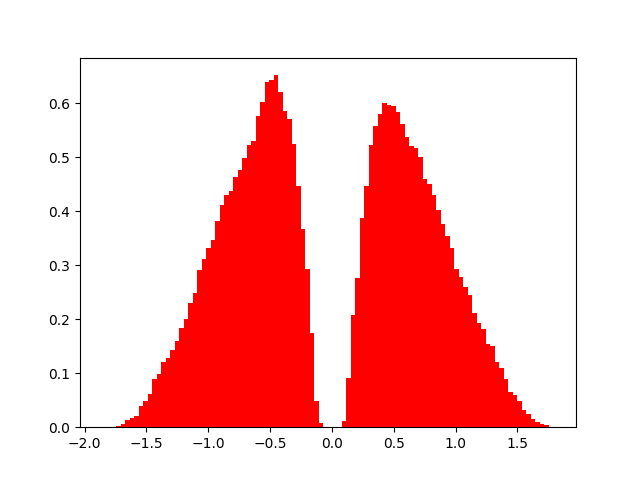
\includegraphics[width=.99\textwidth,trim={3cm 0 0 0},clip]{Chapters/Ch3-Simulations/normalizing_flows/pics/MeetingFigures/Bobby/QT/feature0_noQT.png}
            %\caption[Placeholder Short text]{(a)}
            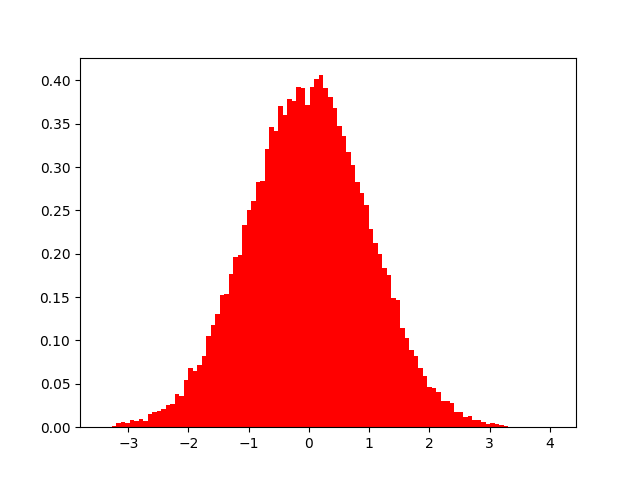
\includegraphics[width=.99\textwidth,trim={3cm 0 0 0},clip]{Chapters/Ch3-Simulations/normalizing_flows/pics/MeetingFigures/Bobby/QT/feature0.png}
    
            %\caption[Placeholder Short text]{(c)}
        \end{minipage}%
        \begin{minipage}{.3\textwidth}
        
            \centering
           % Electron
            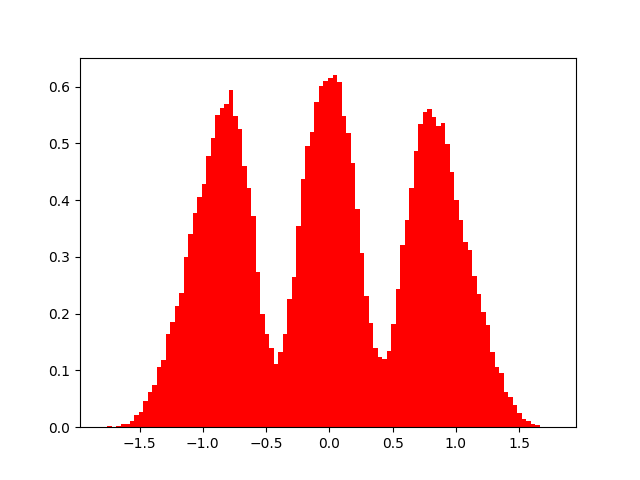
\includegraphics[width=.99\textwidth,trim={3cm 0 0 0},clip]{Chapters/Ch3-Simulations/normalizing_flows/pics/MeetingFigures/Bobby/QT/feature1_noQT.png}
            %\caption[Placeholder Short text]{(a)}
            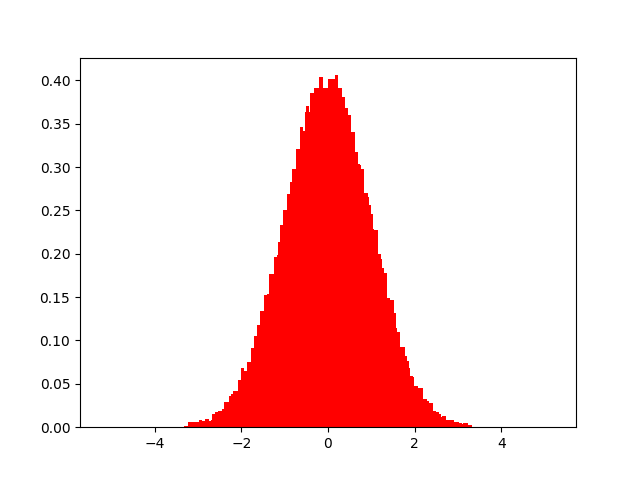
\includegraphics[width=.99\textwidth,trim={3cm 0 0 0},clip]{Chapters/Ch3-Simulations/normalizing_flows/pics/MeetingFigures/Bobby/QT/feature1.png}
    
            %\caption[Placeholder Short text]{(c)}
        \end{minipage}%
        \begin{minipage}{.3\textwidth}
        
            \centering
           % Electron
            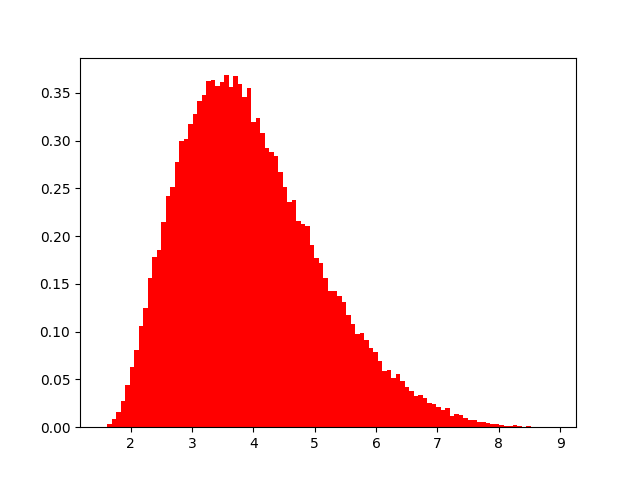
\includegraphics[width=.99\textwidth,trim={3cm 0 0 0},clip]{Chapters/Ch3-Simulations/normalizing_flows/pics/MeetingFigures/Bobby/QT/feature2_noQT.png}
            %\caption[Placeholder Short text]{(a)}
            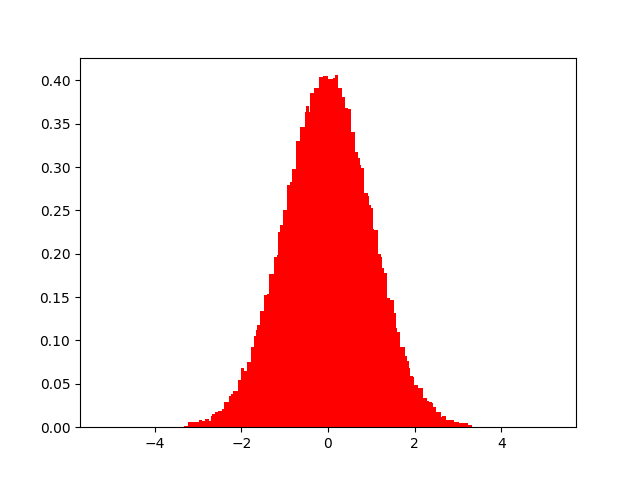
\includegraphics[width=.99\textwidth,trim={3cm 0 0 0},clip]{Chapters/Ch3-Simulations/normalizing_flows/pics/MeetingFigures/Bobby/QT/feature2.png}
    
            %\caption[Placeholder Short text]{(c)}
        \end{minipage}%
        \caption[Placeholder Short text]{Feature distributions before (top) and after (bottom) quantile transforms}
        \label{fig:16features5}
    \end{figure}

        
        Quantile transformations, also known as quantile-quantile (QQ) mapping, play a vital role in statistical analysis. Essentially, the method involves transforming the data to follow a uniform distribution, which is then inverted to follow any other specified distribution. Formally, given a random variable $X$ and its cumulative distribution function $F$, the transformed variable $X^*$ is defined as $X^* = F^{-1}(F(X))$, where $F^{-1}$ is the quantile function of the target distribution. The power of quantile transformations lies in their ability to transform data to follow any desired shape, which makes them especially useful in areas such as machine learning, where they are used for data normalization and generative modeling.

        \begin{figure}[H]
        \centering
        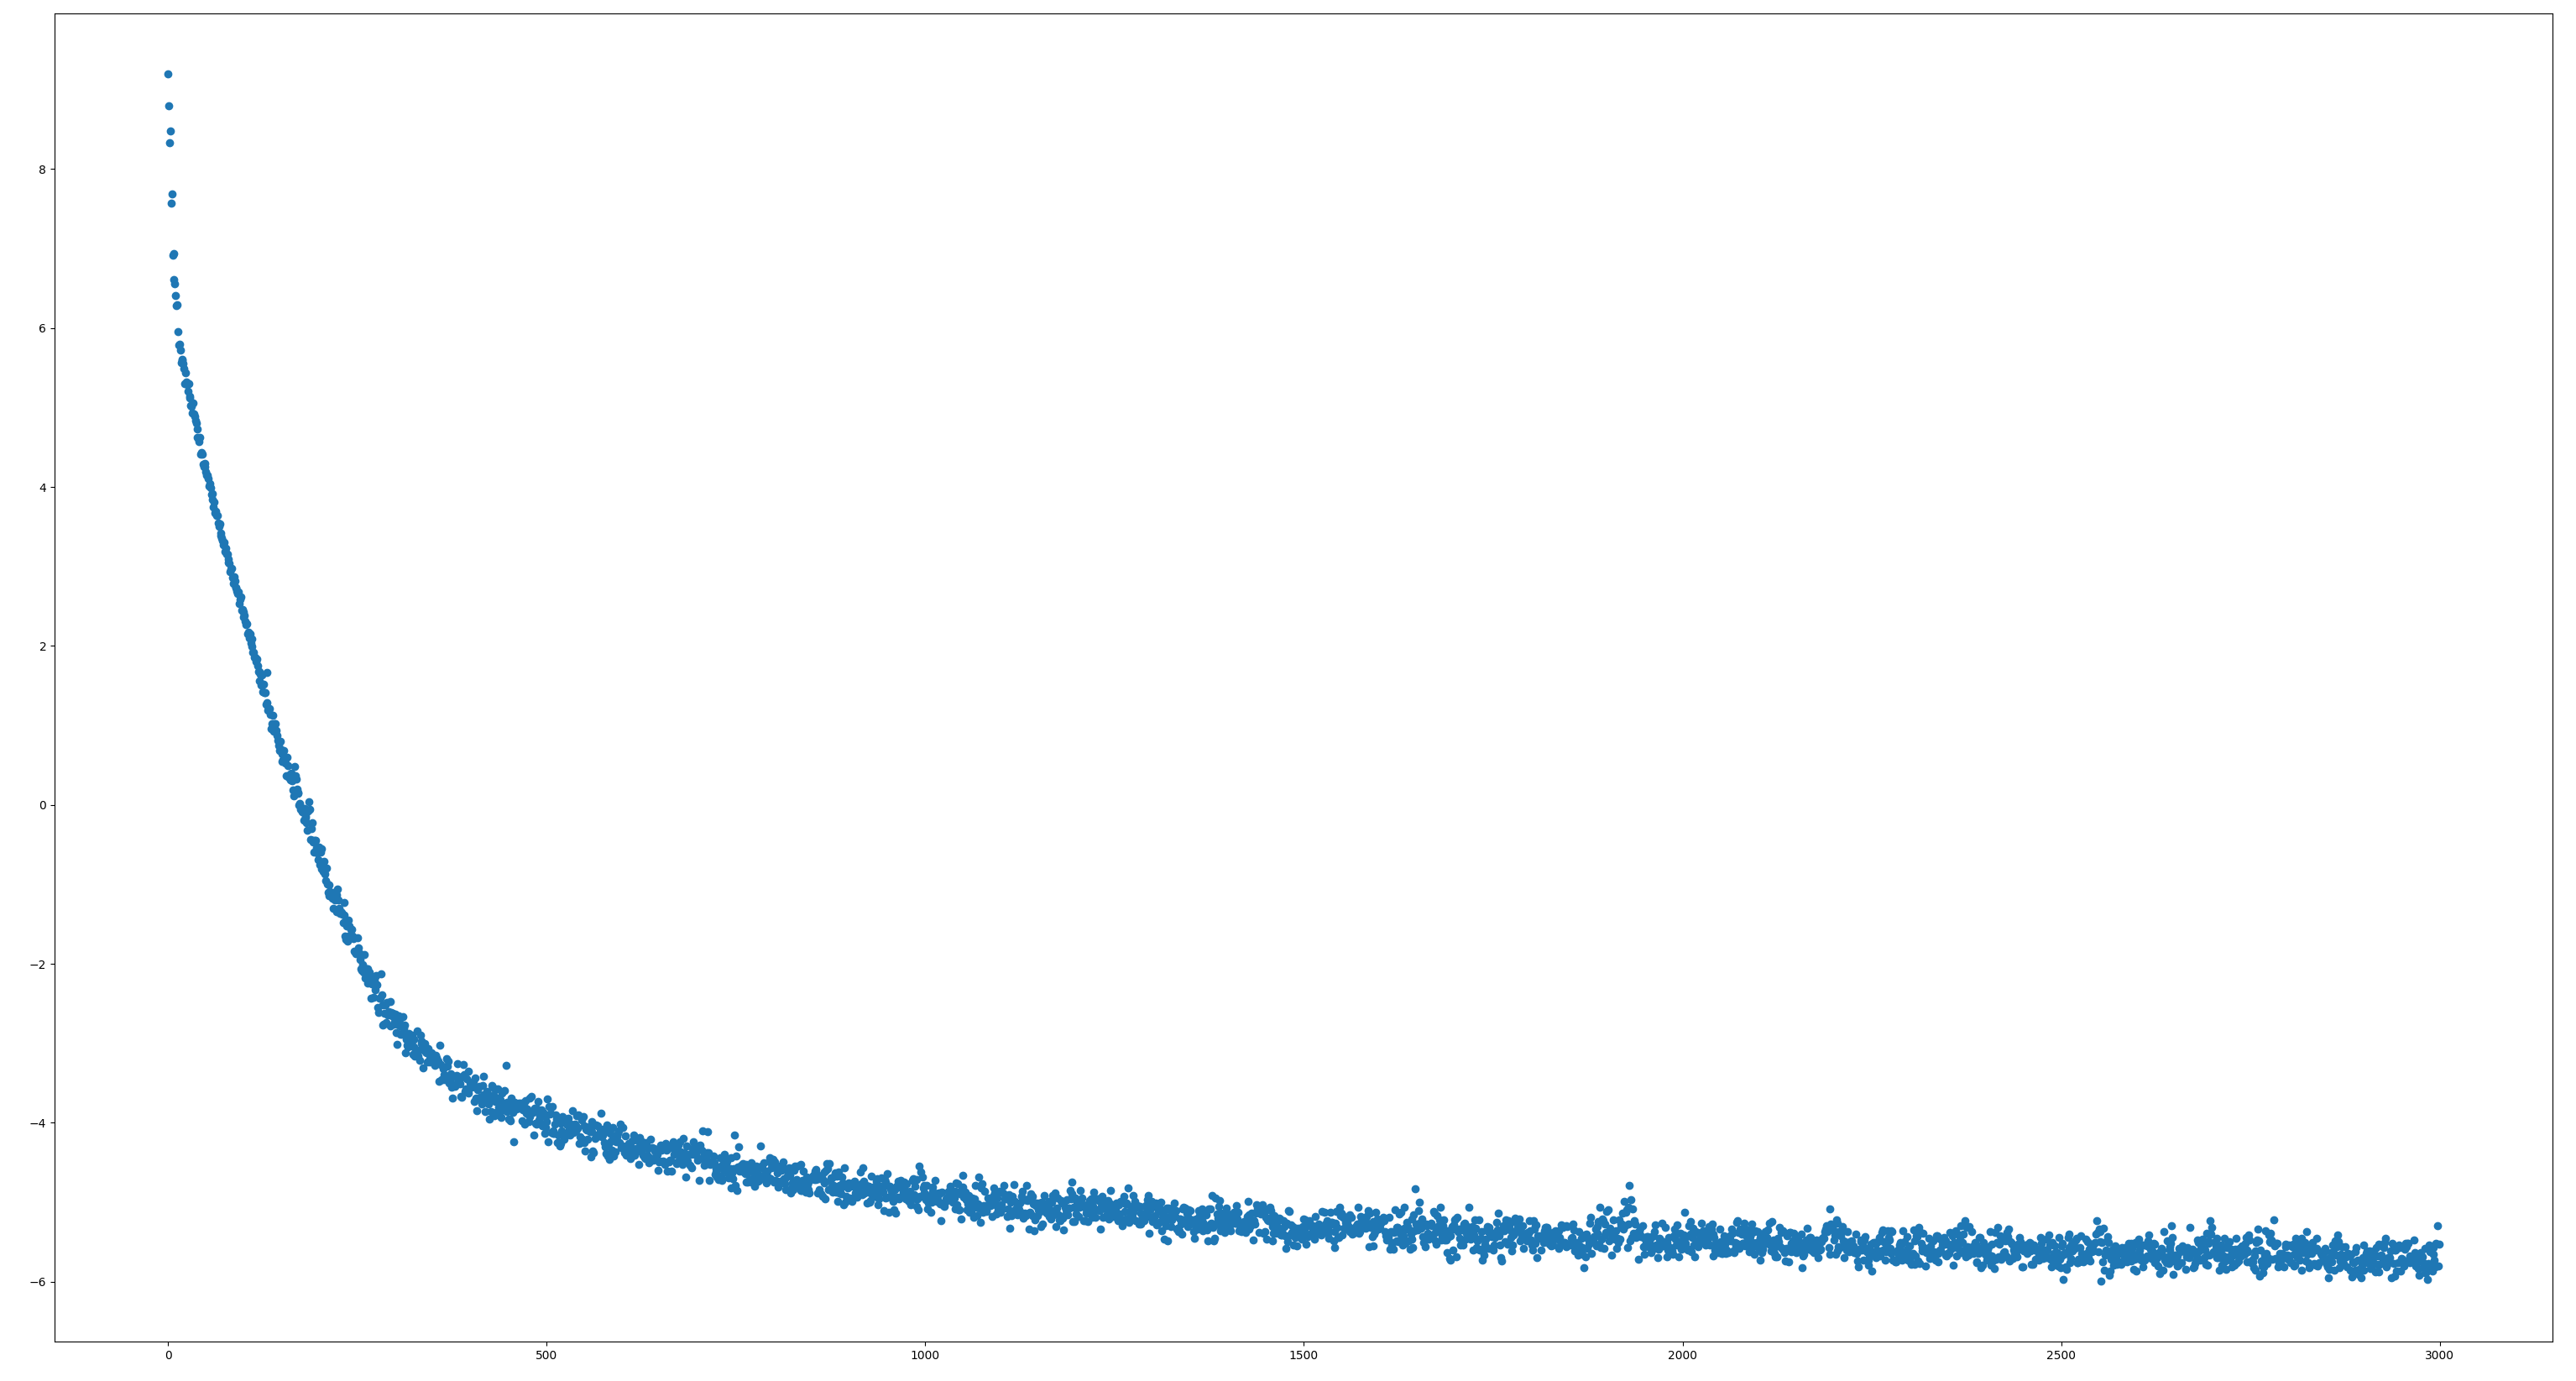
\includegraphics[width = 0.5\textwidth]{Chapters/Ch3-Simulations/normalizing_flows/pics/MeetingFigures/Bobby/LearningRate/learning_rate_25e-5_with_QT.png}
        \label{fig: jul8_pion_comparison4}
        \caption[Placeholder Short text]{Epoch (horizontal) vs Training Loss (vertical). Training loss vs. epoch with LR=2.5e-4, using Quantile Transforms }
        \end{figure}



    \subsubsection{Forward Results from Trained Model}
        Figure \ref{fig:16features} shows the feature distributions of samples from this trained model, with each plot also showing the Earth Mover's Distance between the NF model data, and sample data from the microphysics distribution.
    
        
        In general, the 16-feature trained NF model produces similar results to the traditional simulation's distribution, but fine details were difficult to reproduce. In particular, hard distribution cutoffs that exist in the traditional distribution due to the enforcement of conservation laws and the physics detector edges were not well learned by the NF model, while smoother distributions were reproduced well.
        
        For a quantitative comparison, Figure \ref{fig:EMD} shows the Earth Mover's Distance between samples from the trained NF model and the traditional physics distribution. In the limit of identical distributions with infinitely many samples, the EMD is zero. Since we are working with only 100K datapoints, rather than report the EMD values by themselves (which can be seen in Figure \ref{fig:16features}), we took the ratio of the NF model - traditional physics distribution EMD value to the EMD value calculated between two sets of 100K datapoints taken from the traditional physics distribution, which had values on the order of 0.005. Thus, a perfectly trained NF model would have an EMD ratio of 1, and as we deviate above 1, we exhibit worse performance. We can see in Figure \ref{fig:EMD} that most features have a ratio of about 3--8, which is not perfect, but demonstrates reasonable agreement in line with what is observed in Figure \ref{fig:16features}. Unfortunately, we do not have the reference of these ratios to define the good sampling.
   
        
        \begin{figure}[H]
            \centering
            \begin{minipage}{.23\textwidth}
            
                \centering
               % Electron
                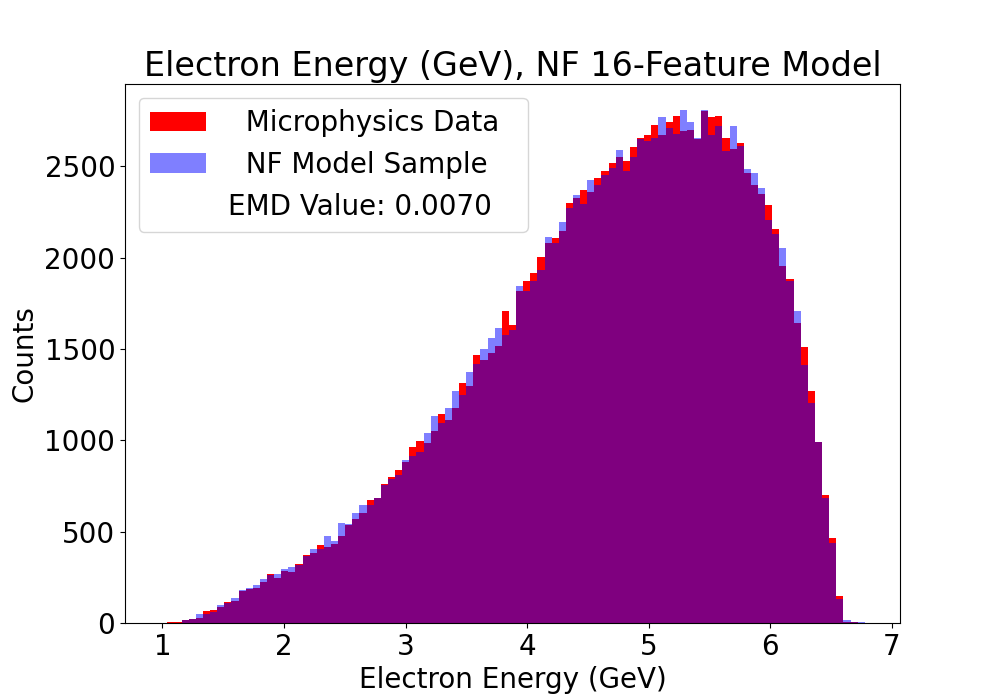
\includegraphics[width=.99\textwidth,trim={3cm 0 0 0},clip]{Chapters/Ch3-Simulations/normalizing_flows/pics/FinalPictures/Features16/Electron_Energy_,_NF_16-Feature_Model.png}
                %\caption[Placeholder Short text]{(a)}
                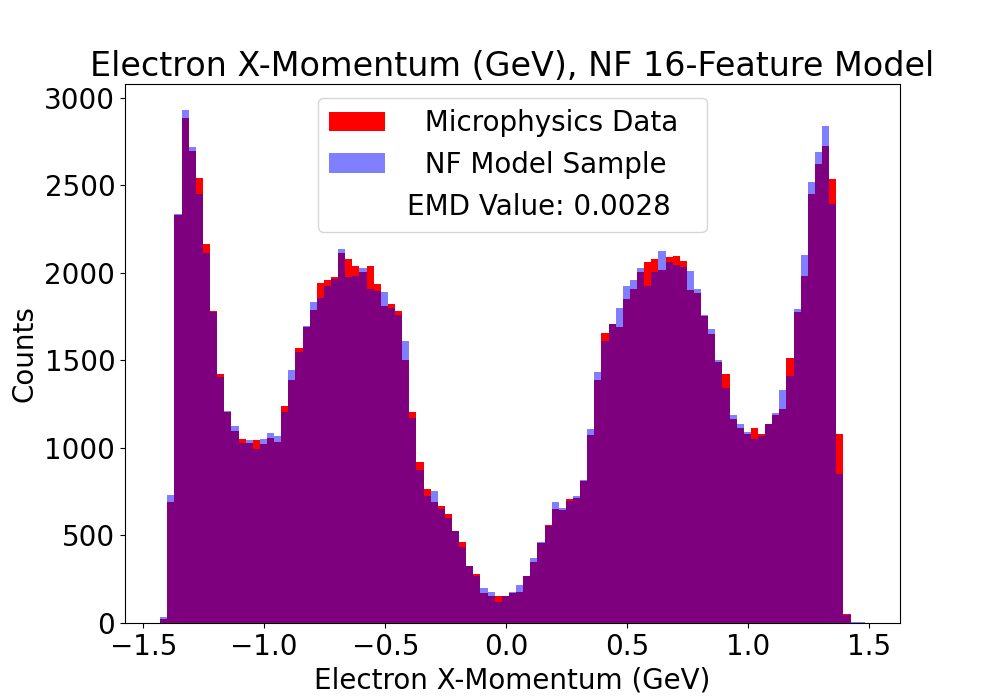
\includegraphics[width=.99\textwidth,trim={3cm 0 0 0},clip]{Chapters/Ch3-Simulations/normalizing_flows/pics/FinalPictures/Features16/Electron_X-Momentum_,_NF_16-Feature_Model.png}
                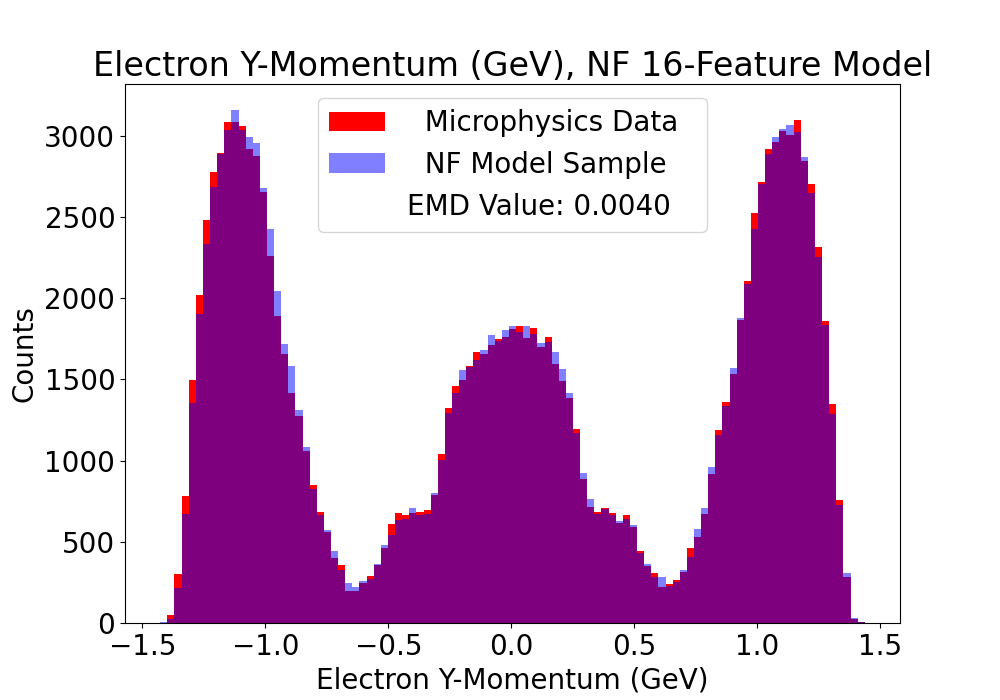
\includegraphics[width=.99\textwidth,trim={3cm 0 0 0},clip]{Chapters/Ch3-Simulations/normalizing_flows/pics/FinalPictures/Features16/Electron_Y-Momentum_,_NF_16-Feature_Model.png}
                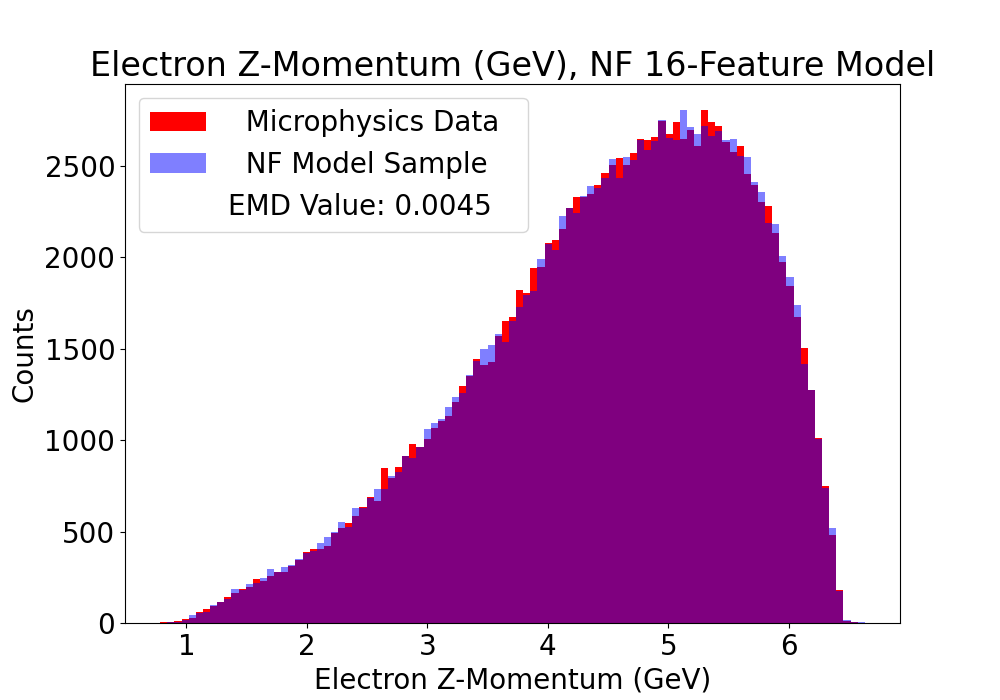
\includegraphics[width=.99\textwidth,trim={3cm 0 0 0},clip]{Chapters/Ch3-Simulations/normalizing_flows/pics/FinalPictures/Features16/Electron_Z-Momentum_,_NF_16-Feature_Model.png}
                %\caption[Placeholder Short text]{(c)}
            \end{minipage}%
            \begin{minipage}{0.23\textwidth}
                \centering
               % Proton
                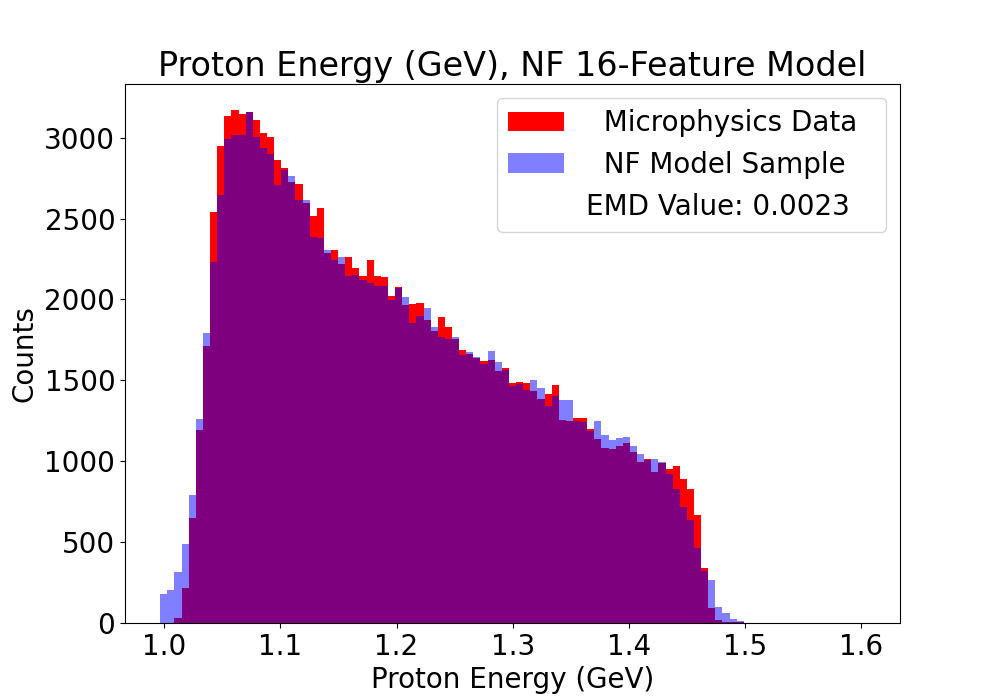
\includegraphics[width=.99\textwidth,trim={3cm 0 0 0},clip]{Chapters/Ch3-Simulations/normalizing_flows/pics/FinalPictures/Features16/Proton_Energy_,_NF_16-Feature_Model.png}
                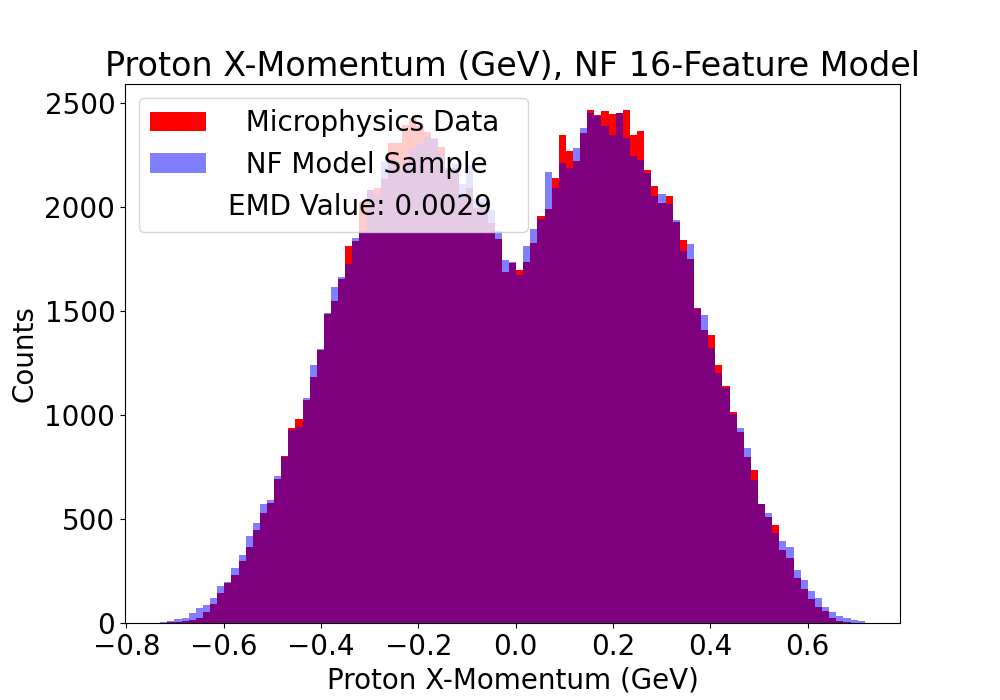
\includegraphics[width=.99\textwidth,trim={3cm 0 0 0},clip]{Chapters/Ch3-Simulations/normalizing_flows/pics/FinalPictures/Features16/Proton_X-Momentum_,_NF_16-Feature_Model.png}
                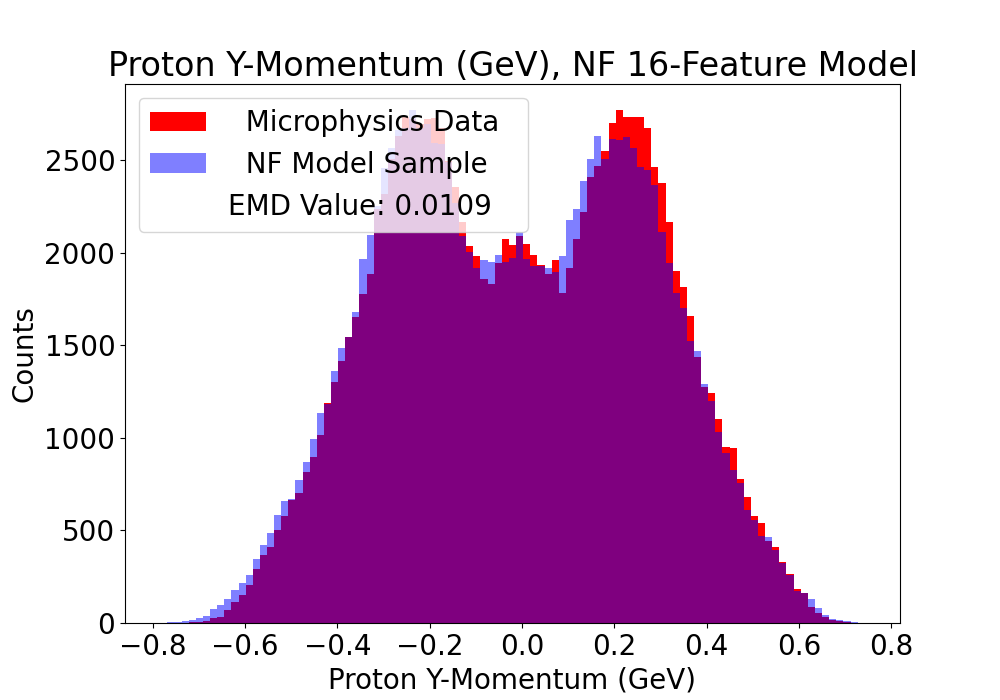
\includegraphics[width=.99\textwidth,trim={3cm 0 0 0},clip]{Chapters/Ch3-Simulations/normalizing_flows/pics/FinalPictures/Features16/Proton_Y-Momentum_,_NF_16-Feature_Model.png}
                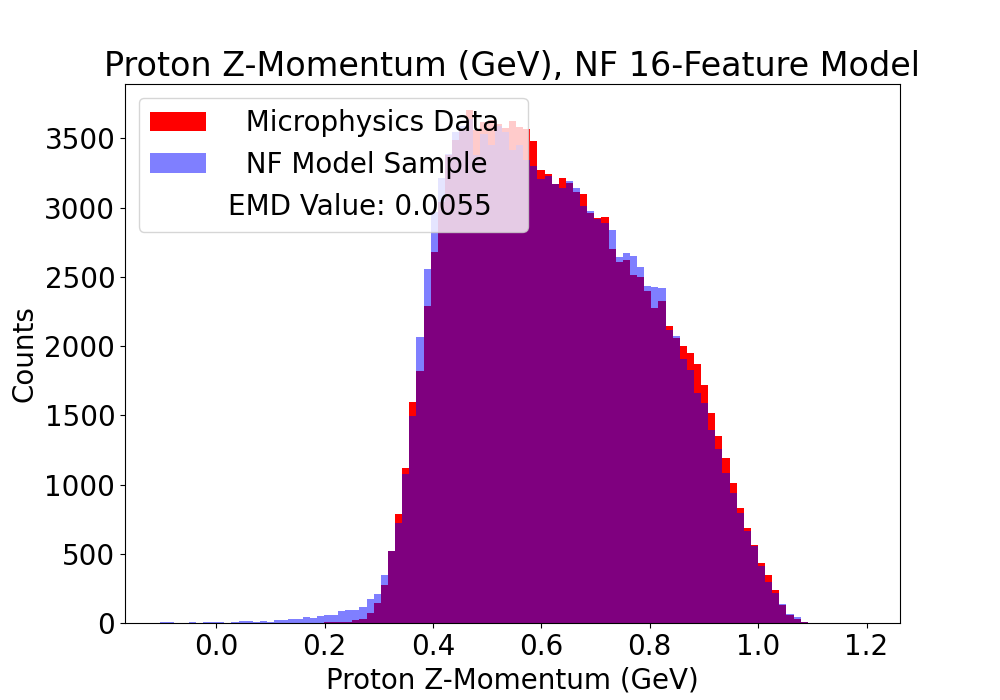
\includegraphics[width=.99\textwidth,trim={3cm 0 0 0},clip]{Chapters/Ch3-Simulations/normalizing_flows/pics/FinalPictures/Features16/Proton_Z-Momentum_,_NF_16-Feature_Model.png}
            \end{minipage}
             \begin{minipage}{0.23\textwidth}
                    \centering
                   % Photon 1
                    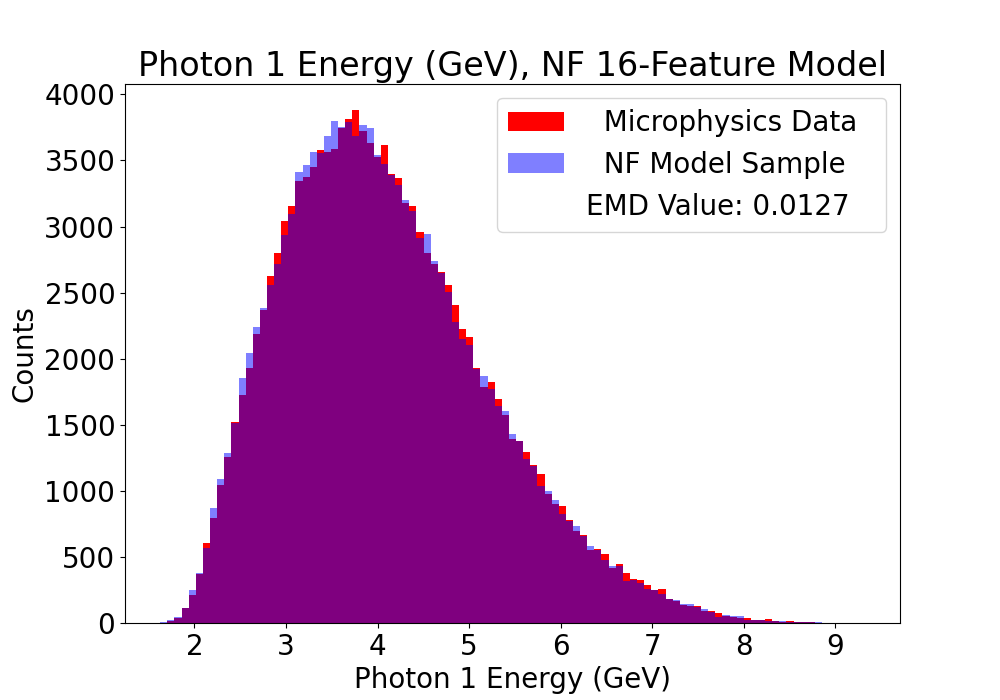
\includegraphics[width=.99\textwidth,trim={3cm 0 0 0},clip]{Chapters/Ch3-Simulations/normalizing_flows/pics/FinalPictures/Features16/Photon_1_Energy_,_NF_16-Feature_Model.png}
                    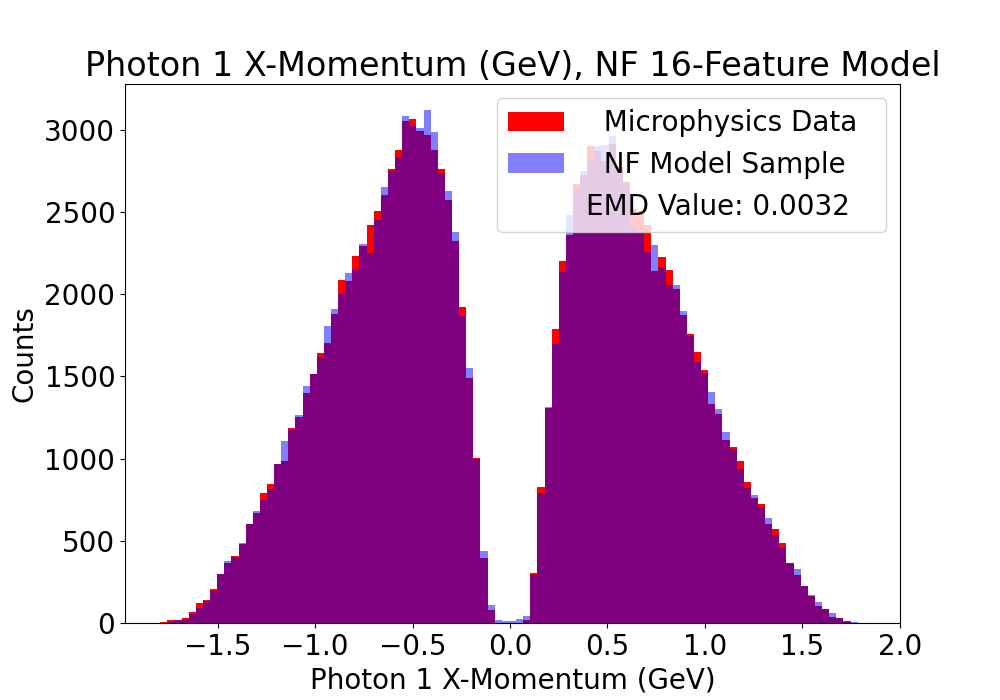
\includegraphics[width=.99\textwidth,trim={3cm 0 0 0},clip]{Chapters/Ch3-Simulations/normalizing_flows/pics/FinalPictures/Features16/Photon_1_X-Momentum_,_NF_16-Feature_Model.png}
                    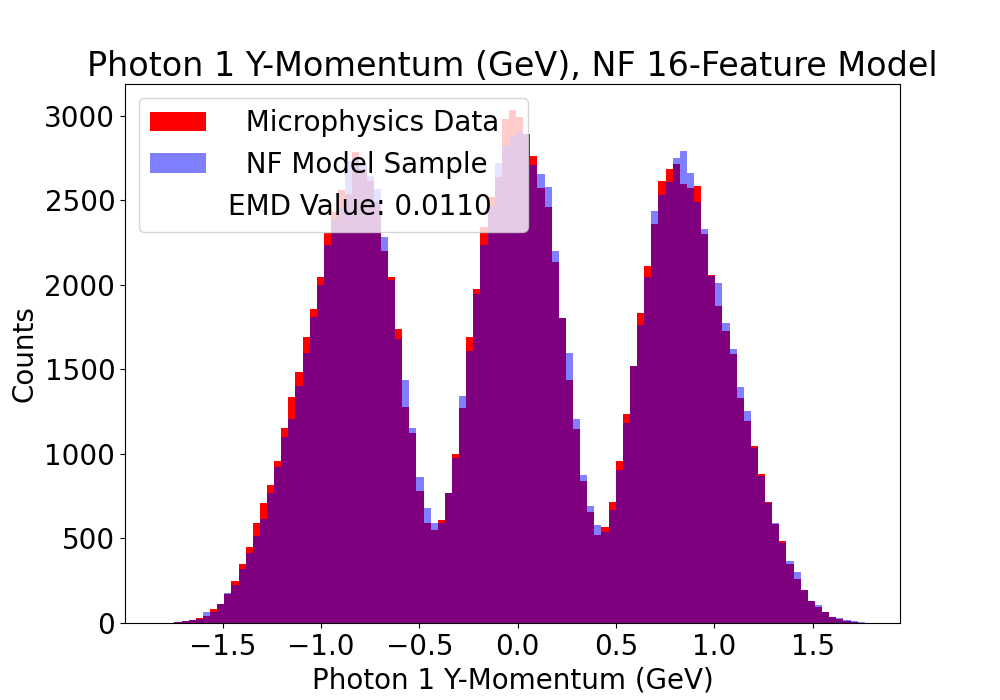
\includegraphics[width=.99\textwidth,trim={3cm 0 0 0},clip]{Chapters/Ch3-Simulations/normalizing_flows/pics/FinalPictures/Features16/Photon_1_Y-Momentum_,_NF_16-Feature_Model.png}
                    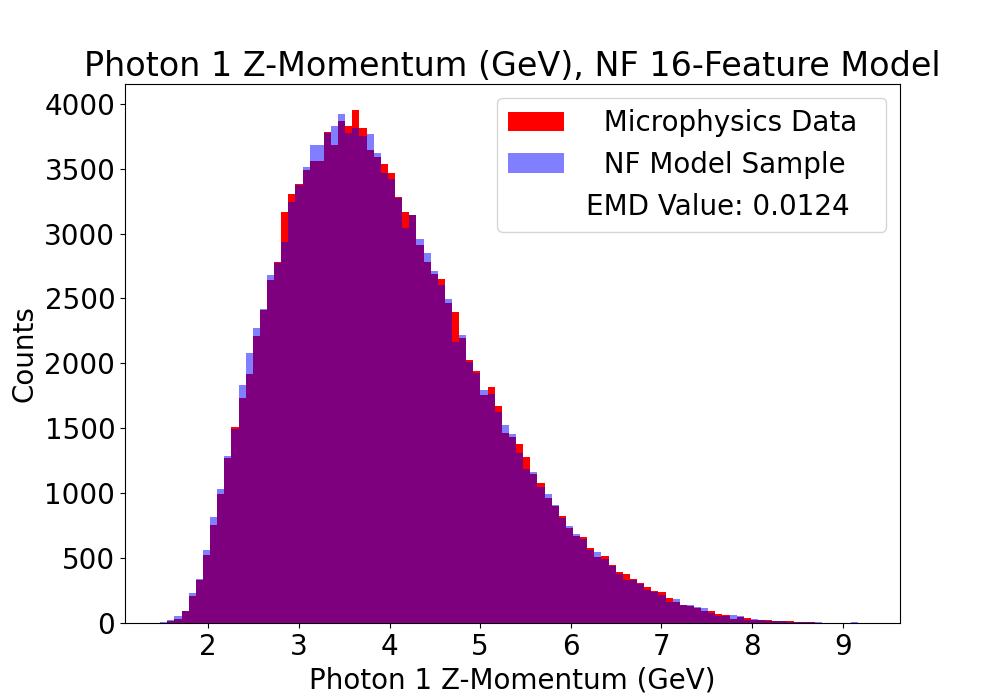
\includegraphics[width=.99\textwidth,trim={3cm 0 0 0},clip]{Chapters/Ch3-Simulations/normalizing_flows/pics/FinalPictures/Features16/Photon_1_Z-Momentum_,_NF_16-Feature_Model.png}
            \end{minipage}
             \begin{minipage}{0.23\textwidth}
                \centering
                %Photon 2
                
                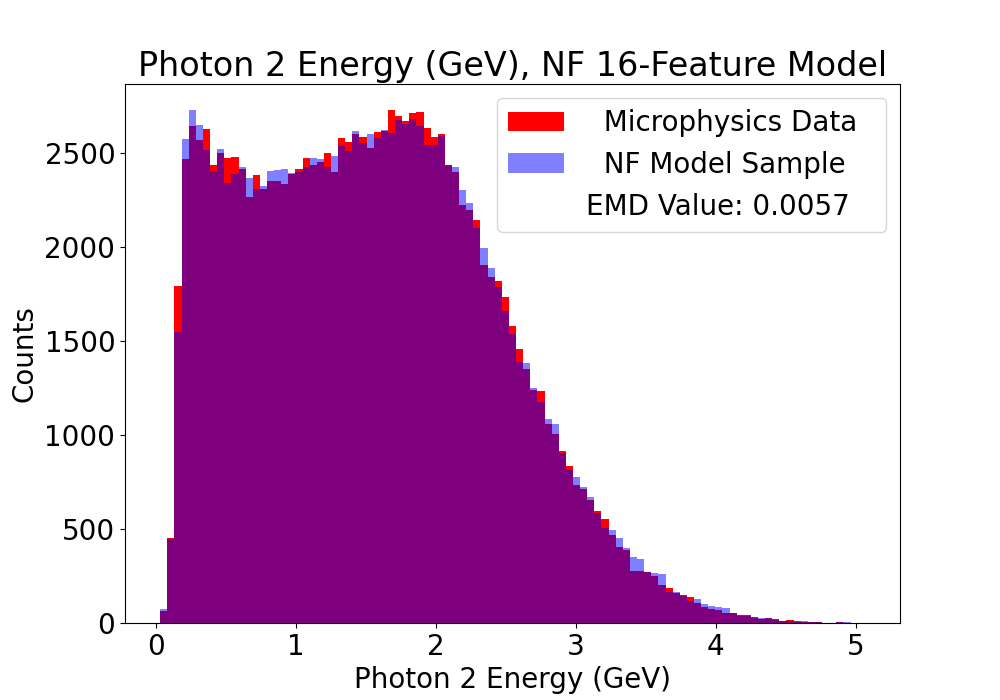
\includegraphics[width=.99\textwidth,trim={3cm 0 0 0},clip]{Chapters/Ch3-Simulations/normalizing_flows/pics/FinalPictures/Features16/Photon_2_Energy_,_NF_16-Feature_Model.png}
                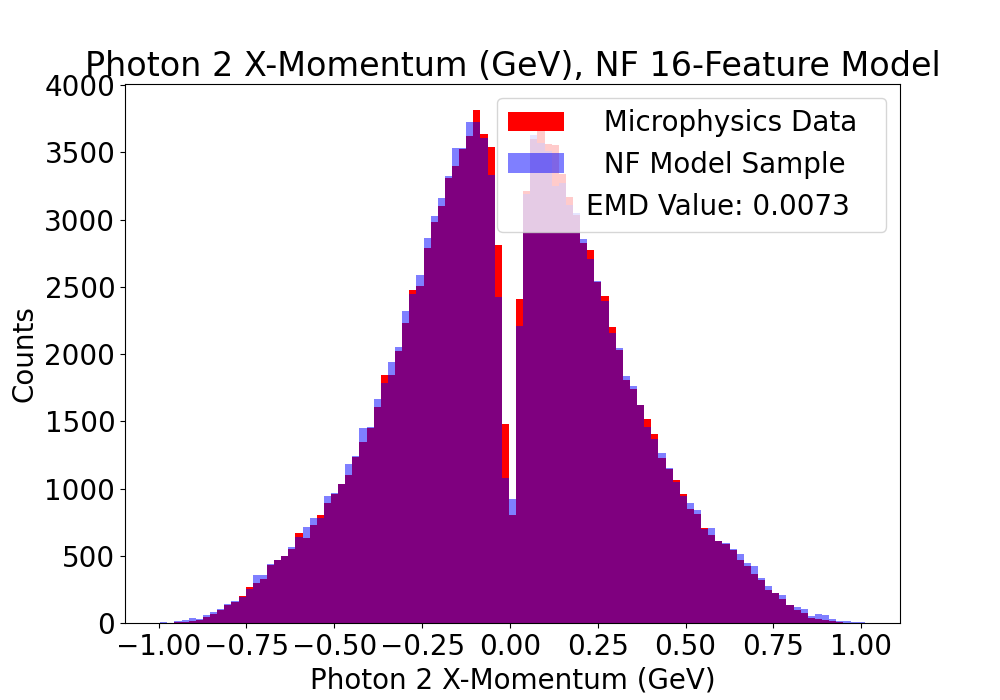
\includegraphics[width=.99\textwidth,trim={3cm 0 0 0},clip]{Chapters/Ch3-Simulations/normalizing_flows/pics/FinalPictures/Features16/Photon_2_X-Momentum_,_NF_16-Feature_Model.png}
                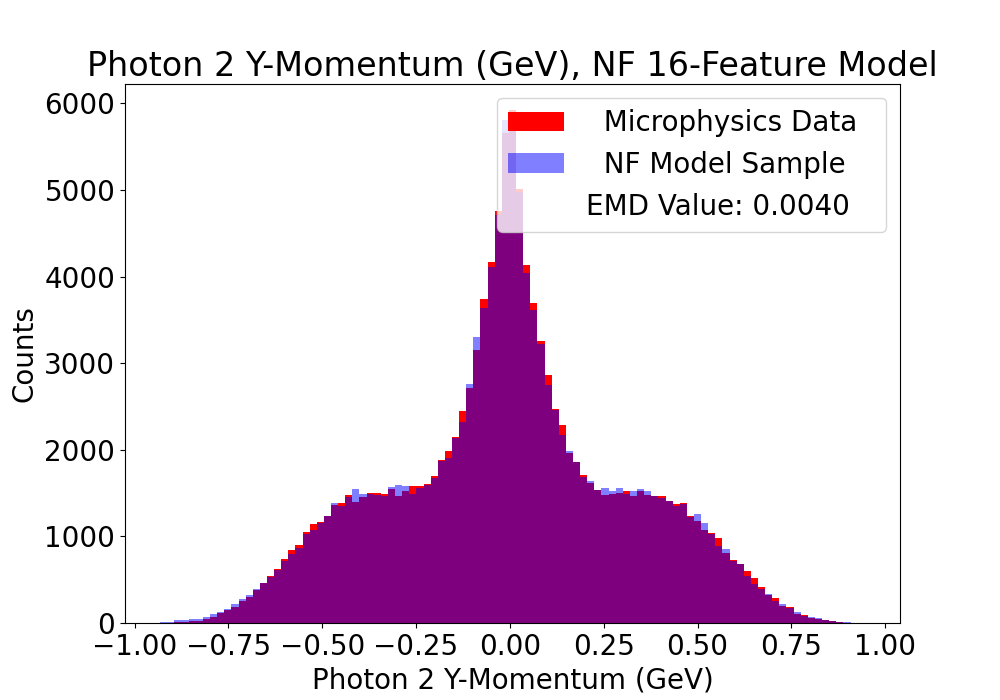
\includegraphics[width=.99\textwidth,trim={3cm 0 0 0},clip]{Chapters/Ch3-Simulations/normalizing_flows/pics/FinalPictures/Features16/Photon_2_Y-Momentum_,_NF_16-Feature_Model.png}
                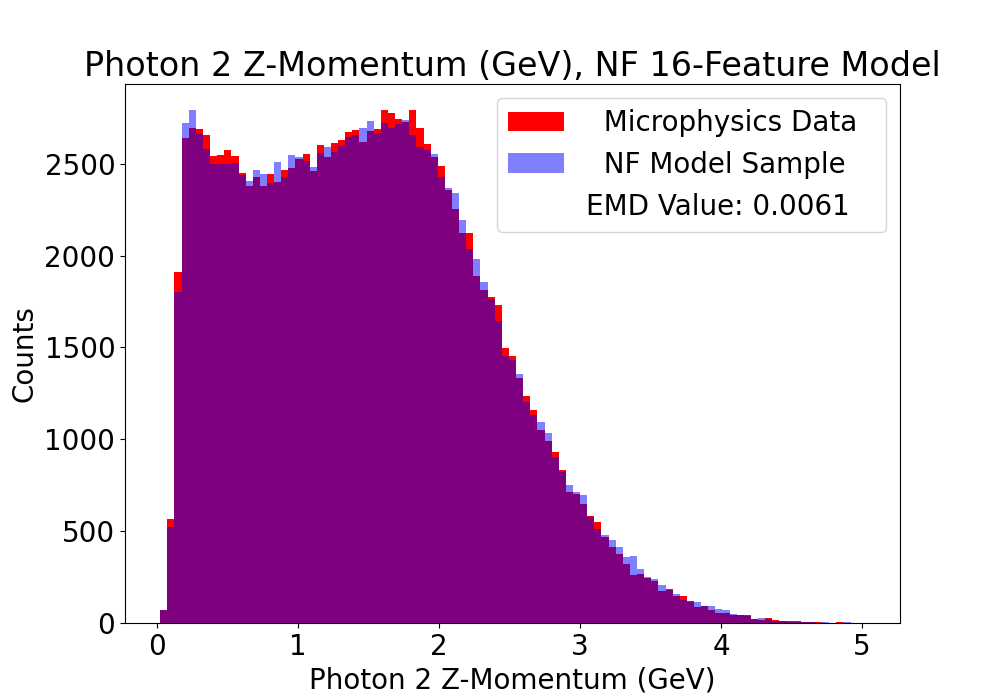
\includegraphics[width=.99\textwidth,trim={3cm 0 0 0},clip]{Chapters/Ch3-Simulations/normalizing_flows/pics/FinalPictures/Features16/Photon_2_Z-Momentum_,_NF_16-Feature_Model.png}
            \end{minipage}
            \caption[Placeholder Short text]{The 1D distributions of all 16 features sampled from our NF model (blue), and from physics simulation (red). Each histogram is normalized to the area, and has 100 bins.}
            \label{fig:16features}
        \end{figure}
        
        
        
        \begin{figure}[H]
            \centering
            %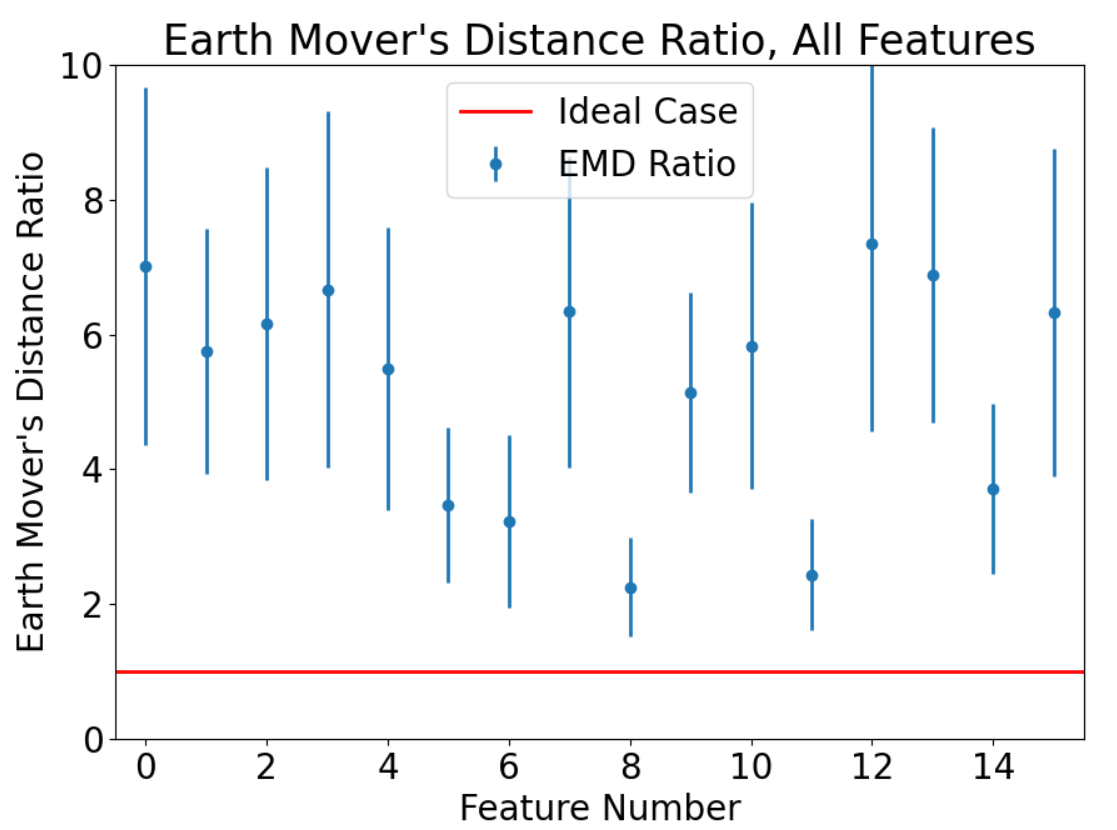
\includegraphics[scale=0.3]{FinalPictures/EMD/EmdRatio.png}
            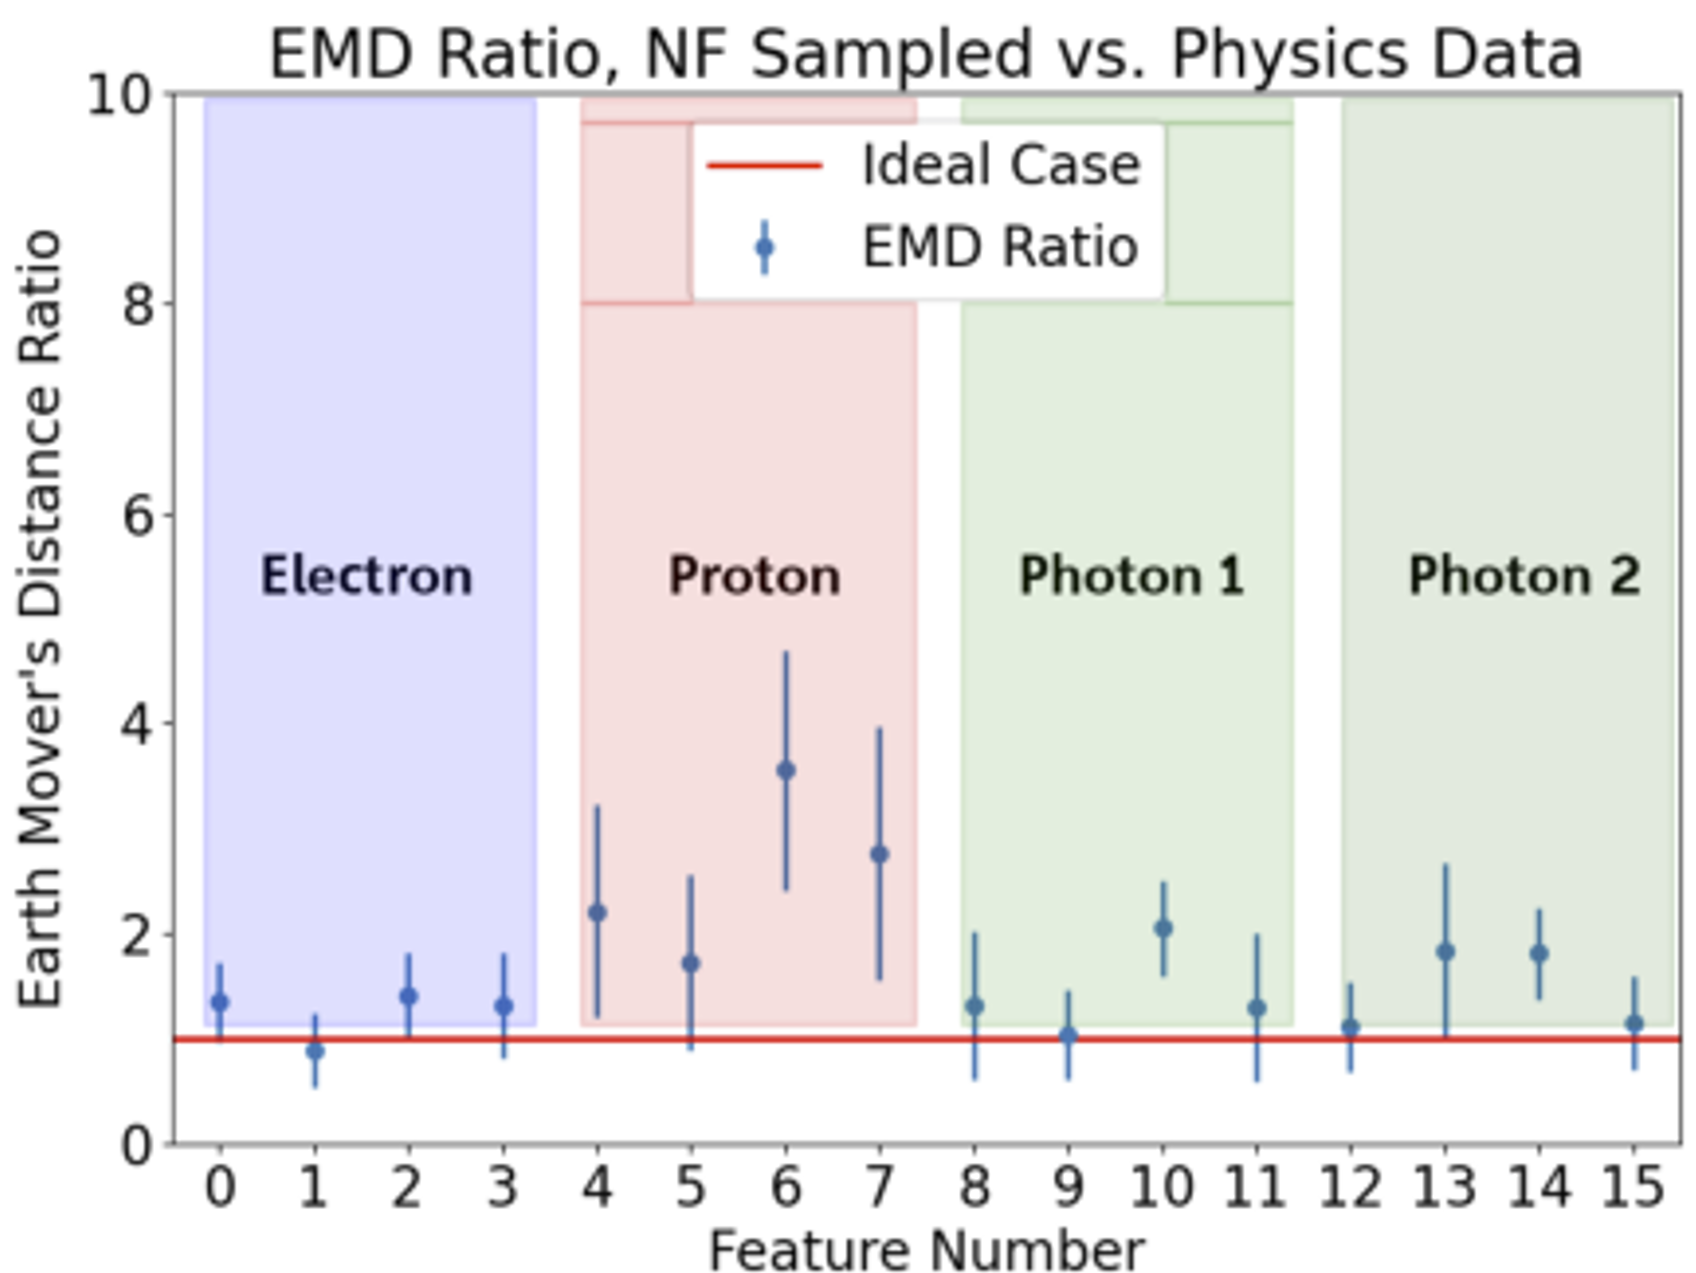
\includegraphics[width=.8\textwidth,trim={0 0 0 0 },clip]{Chapters/Ch3-Simulations/normalizing_flows/pics/FinalPictures/EMD/EMD_updated.png}
            \caption[Placeholder Short text]{The EMD ratios of all 16 features between the NF generated distributions and sample from physics simulation. The points are the average EMD ratios of 10 different subsample calculations; the error bars are the standard deviations of the sets. If the model were perfect, all points would have value 1; deviation from 1 indicates worse performance.}
            \label{fig:EMD}
        \end{figure}
        
        To understand the shortcomings of the trained model, we consider 2-Dimensional distributions in  Figure \ref{fig:2D}. We can see that while some distributions are reproduced well, the fine detail and hard cutoffs that exist in some feature spaces are not learned sharply by the model and result in haziness. Specifically, only certain combinations of particle momenta are measurable due to the physical limitations of our real-world detectors (and hence, our computer-modeled detectors in the traditional microphysics simulations) as well as due to physics conservation law constraints. However, we have yet to incorporate these constraints into our NF model training, and so the samples generated from this trained model exist in traditionally empty regions of phase space. One solution to this issue is to implement filtering after sampling from the model, but given the already slow sampling rate, this would further decrease the speed advantage offered by the normalizing flow method. Work is ongoing to incorporate these constraints in the training of the model itself.
        
        \begin{figure}[H]
            \centering
            \begin{minipage}{.3133\textwidth}
            
                \centering
               % Electron
                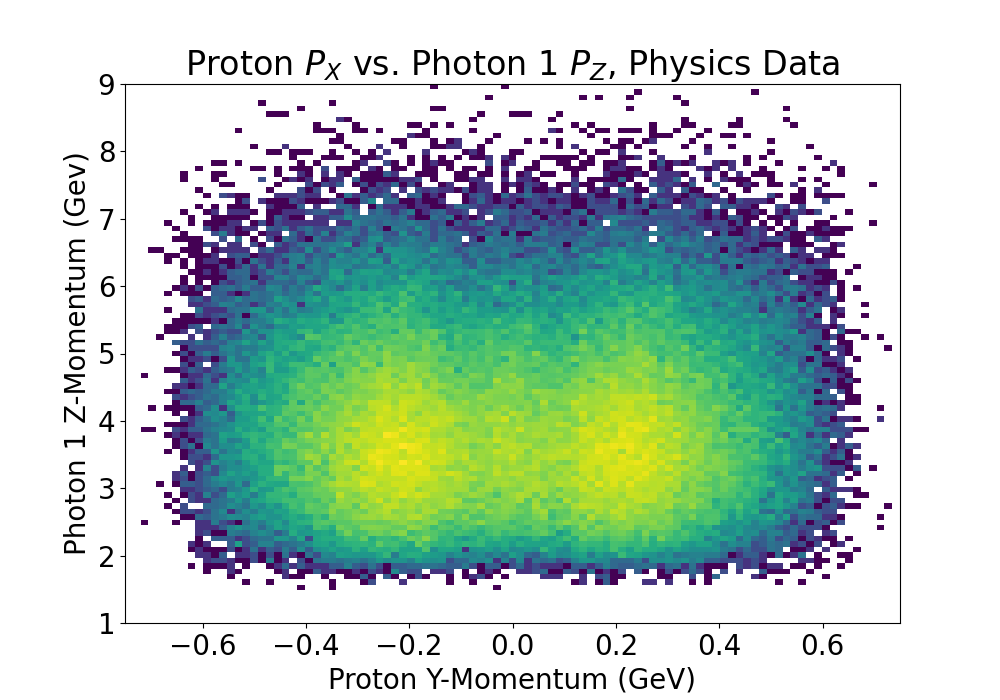
\includegraphics[width=.99\textwidth,trim={0 0 0 0},clip]{Chapters/Ch3-Simulations/normalizing_flows/pics/FinalPictures/Hists2D/Proton_P_X_vs_Photon_1_P_Z,_Physics_Data.png}
                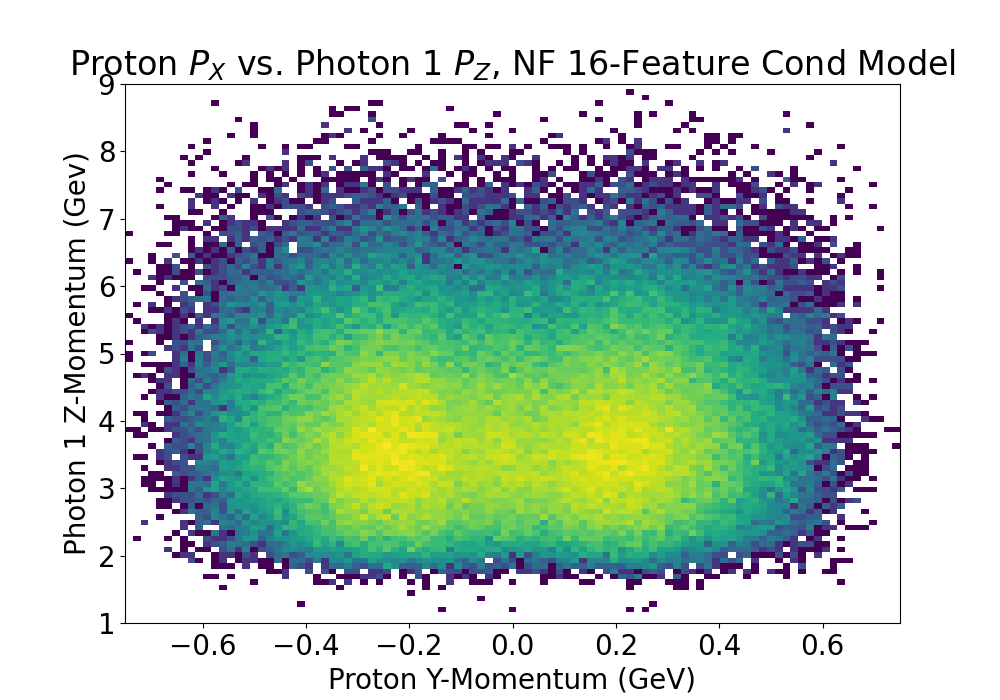
\includegraphics[width=.99\textwidth,trim={0 0 0 0},clip]{Chapters/Ch3-Simulations/normalizing_flows/pics/FinalPictures/Hists2D/Proton_P_X_vs_Photon_1_P_Z,_NF_16-Feature_Cond_Model.png}
        
                %\caption[Placeholder Short text]{(c)}
            \end{minipage}%
            \begin{minipage}{0.3133\textwidth}
                \centering
               %Feature Distributions from Traditional Microphysics Simulations
                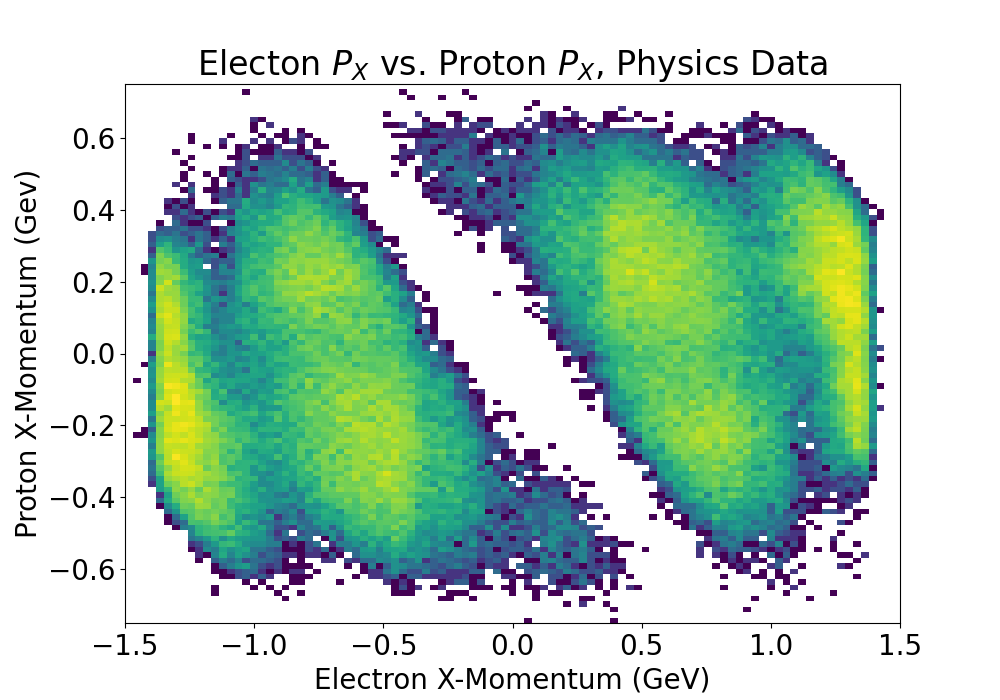
\includegraphics[width=.99\textwidth,trim={0 0 0 0},clip]{Chapters/Ch3-Simulations/normalizing_flows/pics/FinalPictures/Hists2D/Electon_P_X_vs_Proton_P_X,_Physics_Data.png}
                %Feature Distributions from NF Model Samples
                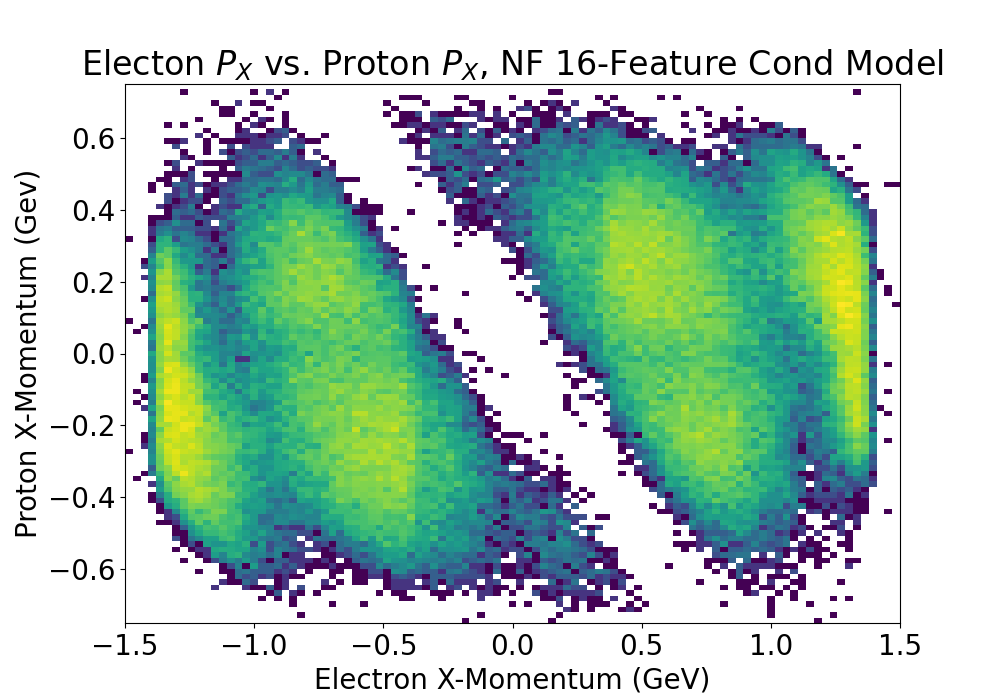
\includegraphics[width=.99\textwidth,trim={0 0 0 0},clip]{Chapters/Ch3-Simulations/normalizing_flows/pics/FinalPictures/Hists2D/Electon_P_X_vs_Proton_P_X,_NF_16-Feature_Cond_Model.png}
                %\caption[Placeholder Short text]{(a)}
                
        
            \end{minipage}
             \begin{minipage}{0.3133\textwidth}
                    \centering
                   % Photon 1
                    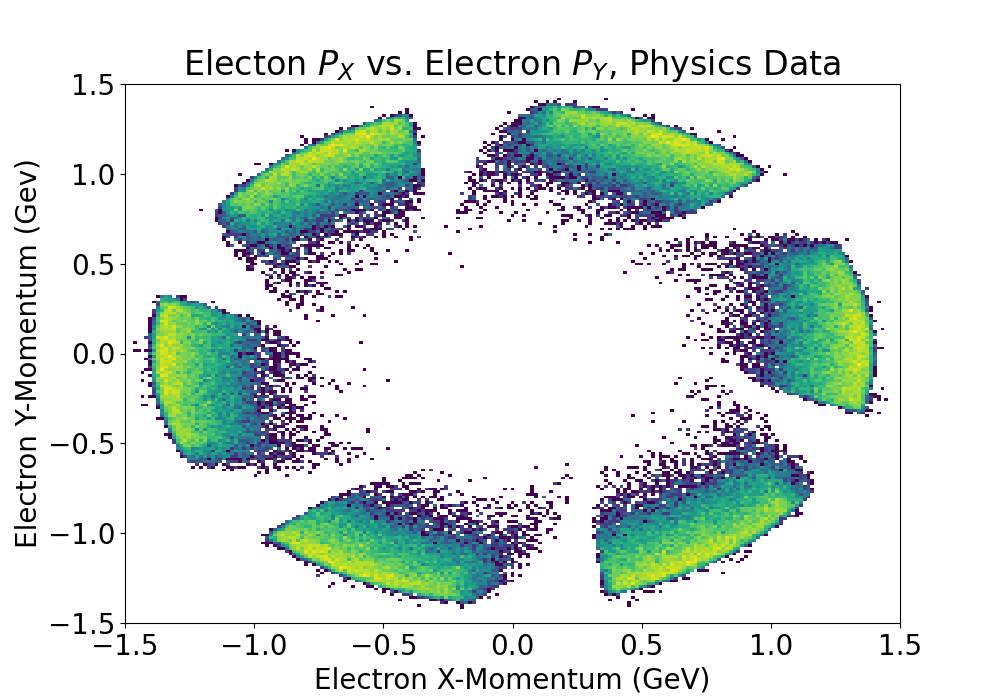
\includegraphics[width=.99\textwidth,trim={0 0 0 0},clip]{Chapters/Ch3-Simulations/normalizing_flows/pics/FinalPictures/Hists2D/Electon_P_X_vs_Electron_P_Y,_Physics_Data.png}
                    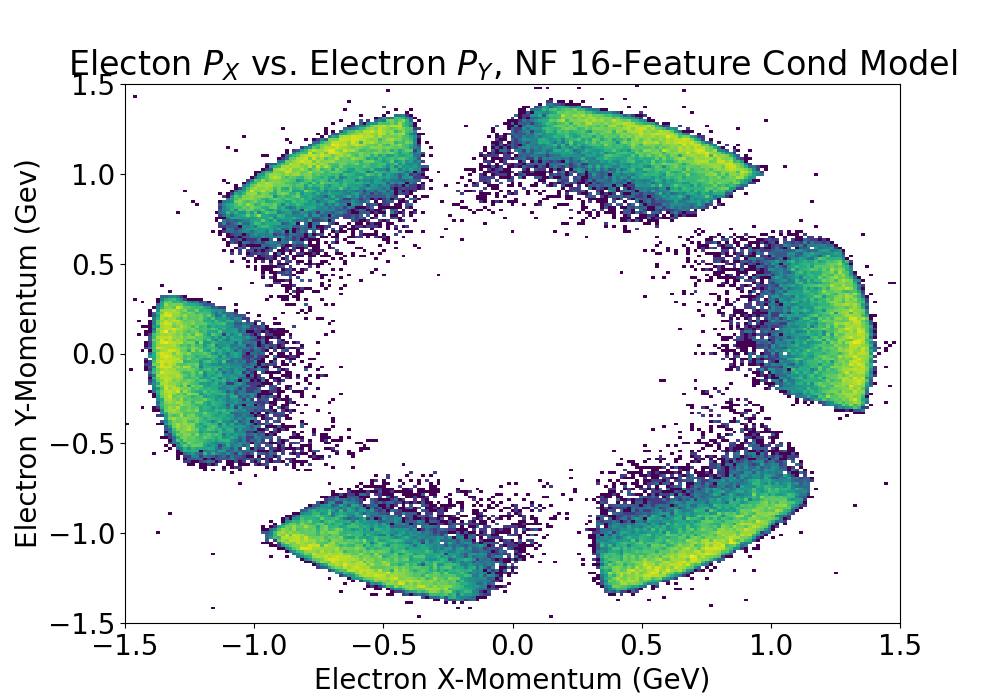
\includegraphics[width=.99\textwidth,trim={0 0 0 0},clip]{Chapters/Ch3-Simulations/normalizing_flows/pics/FinalPictures/Hists2D/Electon_P_X_vs_Electron_P_Y,_NF_16-Feature_Cond_Model.png}
        
            \end{minipage}
            \caption[Placeholder Short text]{ 2-Dimensional distributions for various features, comparing the data from the traditional physics simulation to the NF sampled data. \textbf{Top} Feature distributions from the traditional physics data set. \textbf{Bottom} Feature distributions from our trained NF model, which should match with the top row. Moving from left to right, we can see that some feature distributions are reproduced well, while others have difficult details that are not well modeled, corresponding to physical detector geometry and physics constraints that the NF model is unaware of. }
            \label{fig:2D}
        \end{figure}
        
        
        To try to improve fine-detail reproduction by our model, we trained a second model with only 4-features, which corresponded to a full description of a simulated electron. We observed some improvement in the fidelity of feature reproduction, in particular, Figure \ref{fig:EMD2} shows that, compared to the 16-feature trained model, the 4-feature model (trained only on electron features) exhibits a 2-4 times lower EMD. Of course, this 4-feature trained model is much more limited in scope, but also is able to produce samples much faster, at a rate of about 170 Hz, compared to 4 Hz for the 16-feature model. Given that it describes fully a simulated electron, this would be useful for generally speeding up simulations, but the correlations between different particles that define specific processes like DV$\pi$P is lost. 
        
        
        \begin{figure}[H]
            \centering
            %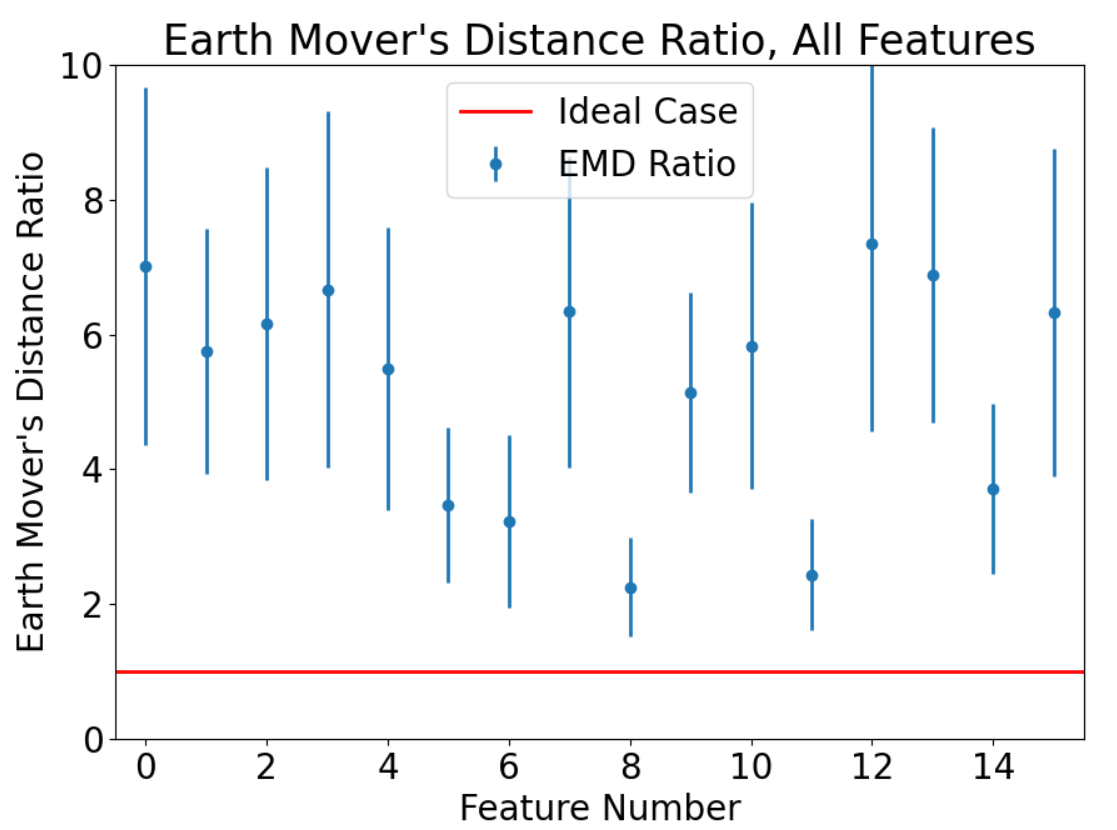
\includegraphics[scale=0.3]{FinalPictures/EMD/EmdRatio.png}
            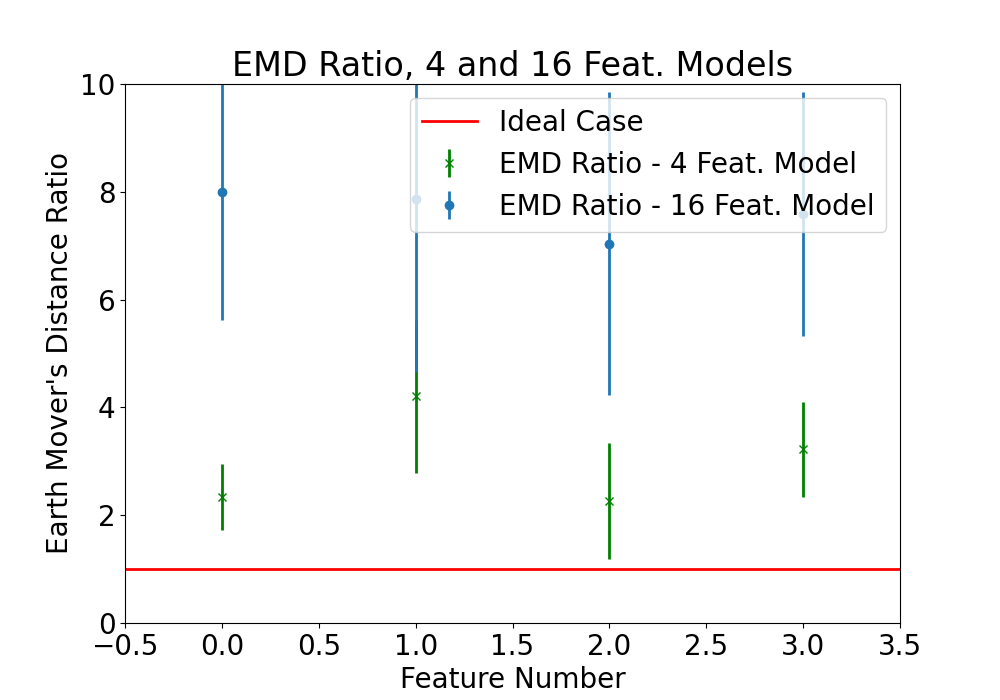
\includegraphics[width=.47\textwidth,trim={ 0 0 0 0},clip]{Chapters/Ch3-Simulations/normalizing_flows/pics/FinalPictures/EMD/emdratio416.png}
            \caption[Placeholder Short text]{The EMD Ratio of selected 4 features between the NF generated distributions and sample from physics simulation when the model was trained using all 16 features as Fig.~\ref{fig:EMD} (blue), and the selected 4 features (green). The 4-Feature trained model shows consistently lower EMD ratio values than the 16-trained model, indicating a better ability to reproduce electron features.}
            \label{fig:EMD2}
        \end{figure}
        
        Comparing to Figure \ref{fig:2D}, we can see from Figure \ref{fig:2D4F} that the 4-feature trained NF model also demonstrates better reproduction of the sharp cutoffs in distributions caused by detector and physics constraints, although still the match is not perfect. Work is ongoing to directly include these constraints in the NF training to decrease these discrepancies.
        
        \begin{figure}[H]
            \centering
             \begin{minipage}{0.31323\textwidth}
                \centering
                Traditional Simulation
                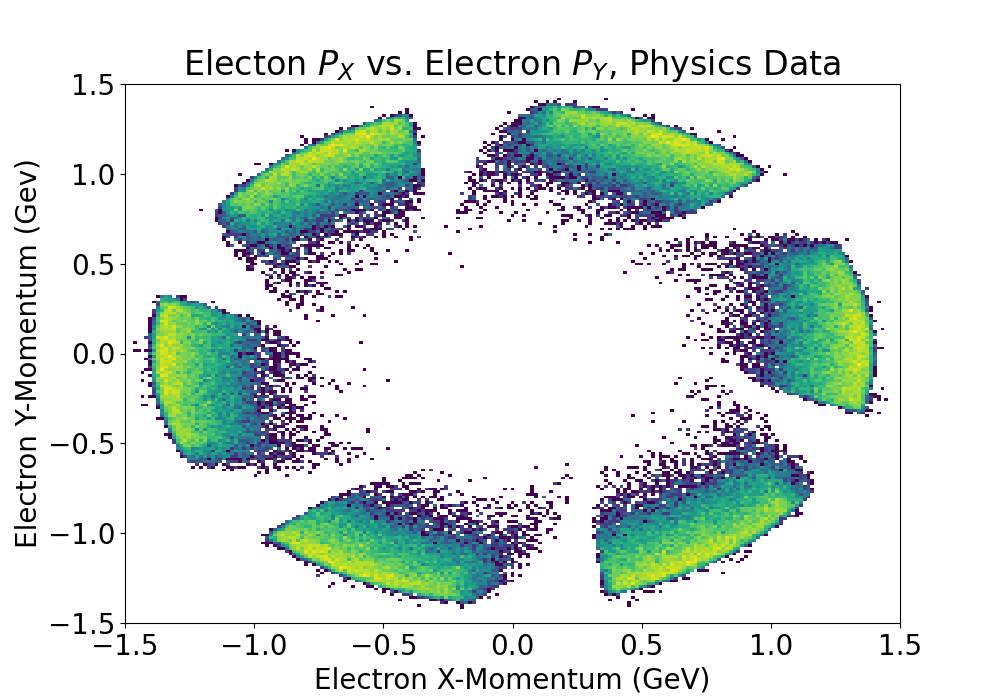
\includegraphics[width=.99\textwidth,trim={0 0 0 0},clip]{Chapters/Ch3-Simulations/normalizing_flows/pics/FinalPictures/Hists2D/Electon_P_X_vs_Electron_P_Y,_Physics_Data.png}
                
            \end{minipage}
                 \begin{minipage}{0.31323\textwidth}
                \centering
                16-Feature Model
                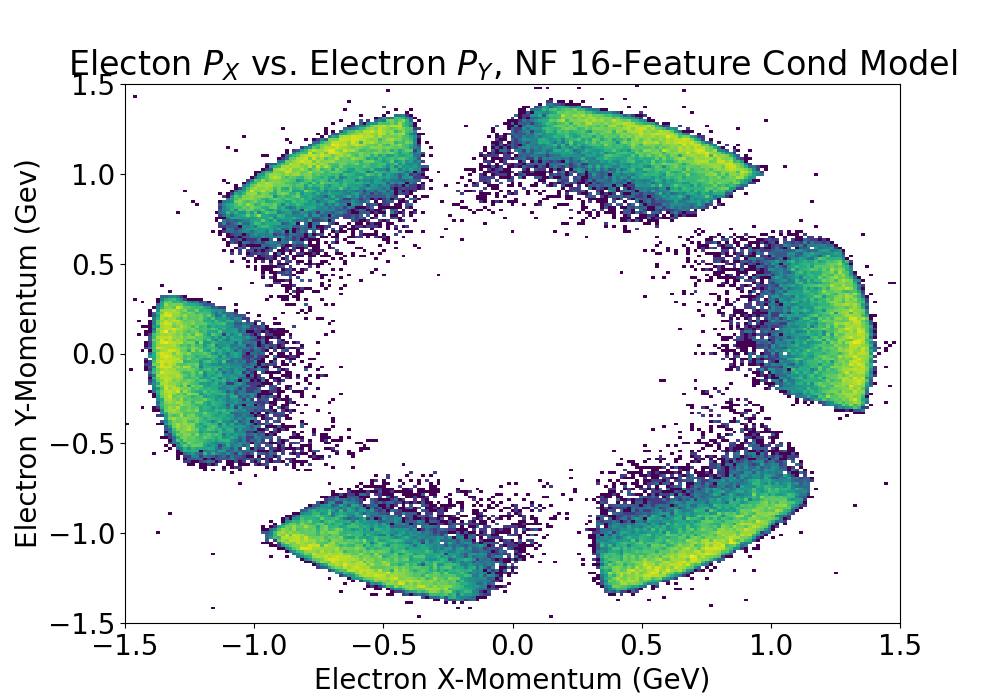
\includegraphics[width=.99\textwidth,trim={0 0 0 0},clip]{Chapters/Ch3-Simulations/normalizing_flows/pics/FinalPictures/Hists2D/Electon_P_X_vs_Electron_P_Y,_NF_16-Feature_Cond_Model.png}
        
            \end{minipage}
                 \begin{minipage}{0.31323\textwidth}
                \centering
                4-Feature\\ Model
               
                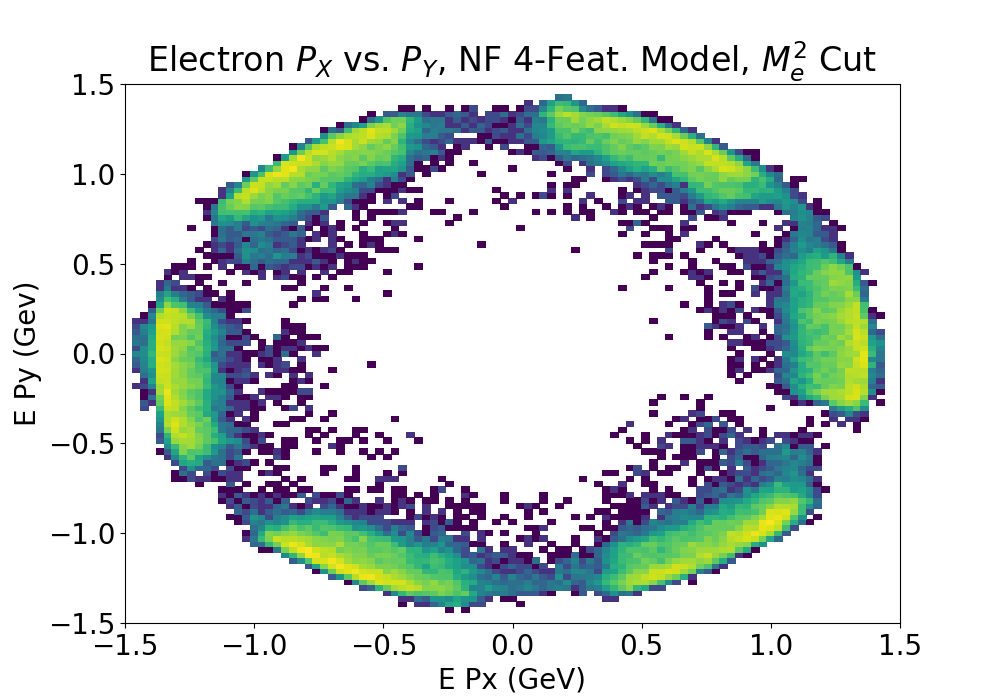
\includegraphics[width=.99\textwidth,trim={0 0 0 0},clip]{Chapters/Ch3-Simulations/normalizing_flows/pics/FinalPictures/2D_Hists_4F/Electron_P_X_vs_P_Y,_NF_4-Feat_Model,_M_e2_Cut.png}
            \end{minipage}
            \caption[Placeholder Short text]{\textbf{Left}: Electron X-Momentum vs. Electron Y-Momentum distribution from the traditional physics simulation dataset. \textbf{Center}: The observed distribution from the 16-Feature trained model, copied from Figure \ref{fig:2D} for reference. We can see considerable disparity between this distribution and the traditional physics distribution. \textbf{Right}: The distribution result from the 4-Feature trained model, which demonstrates far greater agreement to the traditional results compared to the 16-Feature model. }
            \label{fig:2D4F}
        \end{figure}
        
        
        Ultimately, we are interested in physics processes rather than just distribution mapping, so we also examined our ability to reconstruct physics quantities from the trained NF model sample data. Figure \ref{fig:protonspions} shows the distribution of calculated proton and pion (calculated from a combination of the photon features) masses from our NF model data, which had no explicit physics constraints in training. We observe a peak at about 0.939 GeV for the proton and 0.136 GeV for the pion, , which is within 0.5\% of the value encapsulated in the traditional physics training dataset. 
        
        
        \begin{figure}[H]
            \centering
            %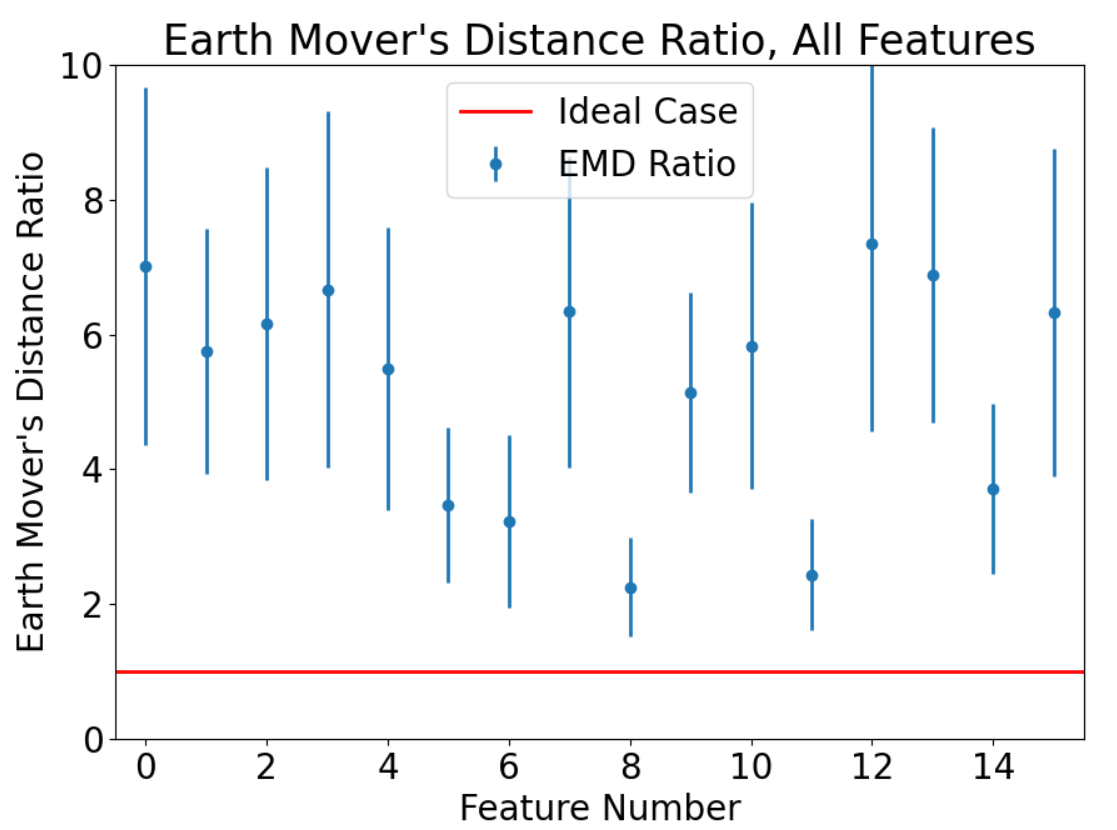
\includegraphics[scale=0.3]{FinalPictures/EMD/EmdRatio.png}
            \label{fig:protons}
        \end{figure}
        
        
        \begin{figure}[H]
            \centering
             \begin{minipage}{0.42349\textwidth}
                \centering
                %Photon 2
                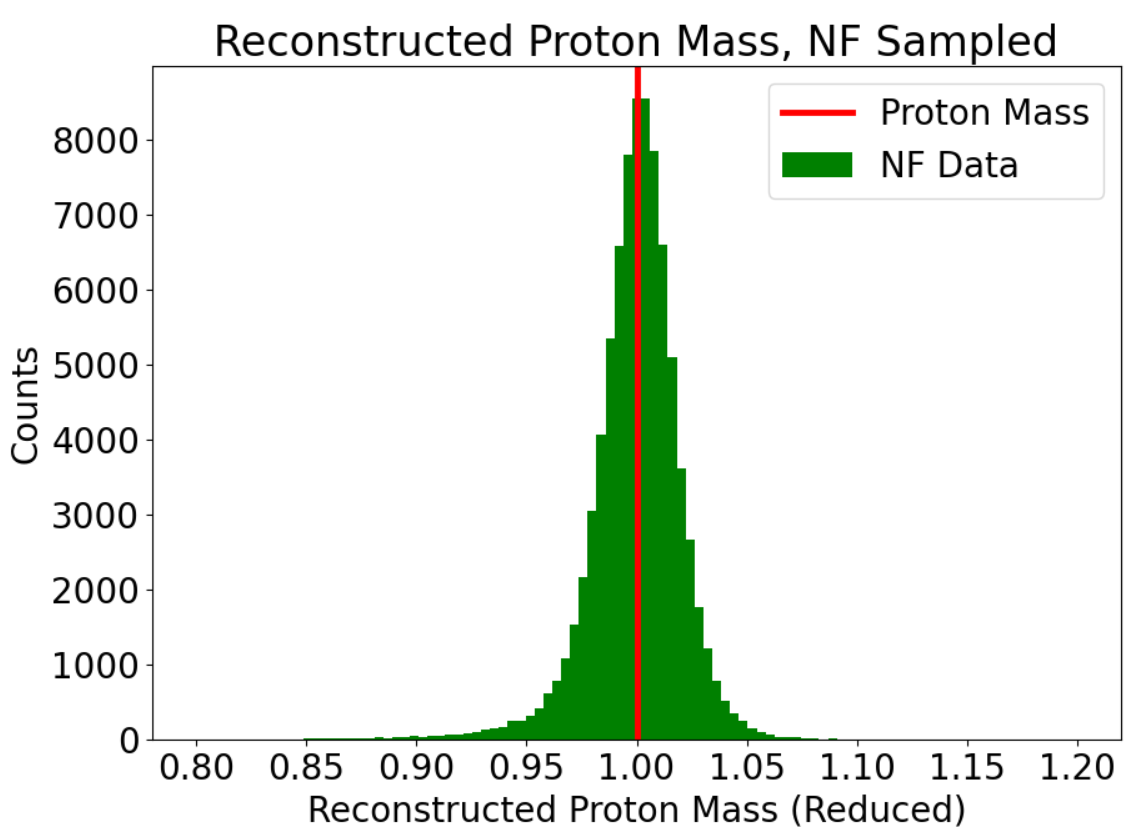
\includegraphics[width=.97\textwidth,trim={ 0 0 0 0},clip]{Chapters/Ch3-Simulations/normalizing_flows/pics/FinalPictures/updated_proton_reduced.png}
        
            \end{minipage}
            \begin{minipage}{0.421245\textwidth}
                \centering
                %Photon 2
                
                \includegraphics[width=.97\textwidth,trim={ 0 0 0 0},clip]{Chapters/Ch3-Simulations/normalizing_flows/pics/FinalPictures/updated_pion_reduced.png}
            \end{minipage}
                \caption[Placeholder Short text]{The distributions of calculated proton mass (left) and pion mass (right) from the 16-Feature trained NF model.  The accepted (true) particle masses are indicated by the red vertical lines, at 0.938 GeV and 0.135 GeV, respectively.
                The peaks from the model are about 1 MeV, or about 0.5\%, shifted away from these true values; while this is small, it is currently unclear what is causing this shift.}
            \label{fig:protonspions}
        \end{figure}
        
        
        Overall, we are able to use a UMNN-MAF architecture to attain reasonable physics distributions far faster than just using traditional physics simulations. At this stage, it is not clear if the 10x speedup afforded by the 16-feature NF model is sufficiently large to justify a decrease in fine-detail resolution. Work is ongoing as to if the model resolution can be improved by including conservation laws as part of training, or if the model can be optimized to generate samples faster. 
        
        On the other hand, the 4-feature model has both higher resolution, and is able to produce samples 1,000 times faster than traditional methods, and so could be very useful immediately to physics research efforts. However, as it is only 4-features, it can only represent one particle, not an entire physics process, but this is still relevant to the study of background processes and noise events in physics experiments, and we are investigating applying this to current CLAS12 research.
        
        The ability of the 16-Feature model to produce realistic protons and pions demonstrates viability for using this method in real physics analysis, but we show there are fine details that the model cannot learn without additional constraints. Work is ongoing to incorporate the physical experimental layout and physics conservation laws into the flow training, which we expect will resolve these discrepancies in fine-detail reproduction, and will lead to a more accurate reproduction of the traditional simulation results, at a far faster speed. 

        \begin{figure}[H]
            \centering
            \subfloat[]{
            \includegraphics[width = 0.45\textwidth]{Chapters/Ch3-Simulations/normalizing_flows/pics/MeetingFigures/Bobby/Reconstructed_Pion_Mass,_16_and_4_Feature_NF_Models_vs_Standard_Simulations.png}
            \label{fig: jul8_pion_comparison5}
            }
            \subfloat[]{
            \includegraphics[width = 0.45\textwidth]{Chapters/Ch3-Simulations/normalizing_flows/pics/MeetingFigures/Bobby/qt-3-4.png}
            \label{fig: jul8_pion_comparison}
            }
            \caption[Placeholder Short text]{Comparison of reconstructed pion mass with different training models and preprocessing methods. The left panel shows the approximation of the standard reconstruction pion mass peak using a 4 feature model and a 16 feature model, where the 4 feature model shows a better fit. The right panel demonstrates a slight improvement in the reproduction of the GEANT4 simulated pion peak when preprocessing the feature set with a quantile transformer before training the normalizing flow.}
            \label{fig:combined_pion_comparison}
        \end{figure}


\subsection{Inverse Problems}

    The conditional normalizing flow takes the base distribution $Y$ and the context $Z$ to learn $X$. How do training and sampling work? 
    
   
    
    
    
    
    \begin{figure}[H]
        \centering
        \begin{minipage}{.5\textwidth}
        
            \centering
           % Electron
            
            %\caption[Placeholder Short text]{(a)}
            \includegraphics[width=.99\textwidth,trim={0 0 0 0},clip]{Chapters/Ch3-Simulations/normalizing_flows/pics/MeetingFigures/Bobby/inverse/gen_Px_1_vs_gen_-_recon_Px_1.png}
            \includegraphics[width=.99\textwidth,trim={0 0 0 0},clip]{Chapters/Ch3-Simulations/normalizing_flows/pics/MeetingFigures/Bobby/inverse/gen_Px_1_vs_gen_-_nf_Px_1.png}
    
            %\caption[Placeholder Short text]{(c)}
        \end{minipage}%
        \begin{minipage}{.5\textwidth}
        
            \centering
           % Electron
            
            %\caption[Placeholder Short text]{(a)}
            \includegraphics[width=.99\textwidth,trim={0 0 0 0},clip]{Chapters/Ch3-Simulations/normalizing_flows/pics/MeetingFigures/Bobby/inverse/gen_Py_1_vs_gen_-_recon_Py_1.png}
            \includegraphics[width=.99\textwidth,trim={0 0 0 0},clip]{Chapters/Ch3-Simulations/normalizing_flows/pics/MeetingFigures/Bobby/inverse/gen_Py_1_vs_gen_-_nf_Py_1.png}
    
            %\caption[Placeholder Short text]{(c)}
        \end{minipage}%
        \caption[Placeholder Short text]{\textbf{TOP:} Truth Event - Reconstructed Event. If standard physics reconstruction algorithms were perfect, we would have a horizontal line at 0 across the distribution (no difference between the reconstructed feature value, and the true feature value, for any event in the data set). \textbf{BOTTOM:} Truth Event - NF estimate of truth event conditional on Reconstructed event values. For the NF to be useful, we would need the difference between the truth event values and the NF estimates to be closer to zero than the differences between just the truth and reconstructed values. However, instead we observe that the spread is about a factor of 2 \textbf{worse} using the NF than not using it at all. }
        \label{fig:16features6}
    \end{figure}
    
    
    I have tried to train the NF to reproduce $x-b$, not $x$ itself because, the 1D distributions of $x-b$'s are more symmetric. This practice clarifies the problem that we have encountered.
    
    Let's focus on only one feature, electron's $p_x$ for example. This time, I used 6 layers of intermediate flows. electron pxshows that the issue in this probabilistic inverse problem.
    The NF is trained to learn $x-b$ distributions, and it did its job by producing $\mathbf{z_6}-\mathbf{b}$ that follows $\mathbf{x}-\mathbf{b}$. Now, we want $\mathbf{z_6}-\mathbf{b}$ to be exactly 0, but in reality we're seeing a larger variance in the sample $\mathbf{z_6}-\mathbf{x}$.
    
    So, this is my guess about what is happening. Let's oversimplify about the difference. For the single elements,
    \begin{align}
        x -b =& ~a = \pm 1\\
        z_6-b =& ~b = \pm 1\\
        z_6 -x =& (z_6-b) - (x-b) = a- b \neq 0
    \end{align}
    We can only make $a$ and $b$ follow the same distribution, i.e., binary distribution, but $a$ and $b$ are mostly independent without a correct guessing of probability on the sign. So, $a-b$'s distributions are actually convolution of two binary distributions, not 0. So this implies that the conditional NF works really well in terms of reproducing collective behavior, but not in the event by event basis that is required for this study. Actually, there is no feature that is directly related to the signs of $x-b$.
    
    
    
    inverse is an ongoing study
    
    We demonstrate a proof of principle for using a normalizing flow to learn a physics process's probability distribution in order to decrease physics simulation computing time and requirements. In this work, we used traditional physics simulations to generate a dataset $\mathbf{x}$ of 5 million data points with each data point having 16 or 4 features.  We take as input a constant 16D or 4D normal distribution $p(\mathbf{z})$, and examine whether the flow model can learn the transformation to $p(\mathbf{x})$ using a random subset of $\mathbf{x}$ for training. We observed a reasonable agreement between the results of the flow-based modeling and traditional physics methods while achieving a computational speedup factor of 10 to 1,000, but the flow is currently unable to reproduce some fine-detailed structures of the physics process.
    
    
    \parencite{Radhakrishnan2020OverparameterizedMemory}



